\documentclass[a4paper]{article}
\usepackage{vntex}
\usepackage{a4wide,amssymb,epsfig,latexsym,multicol,array,hhline,fancyhdr}
% \usepackage{geometry}
%  \geometry{
%  a4paper,
%  total={160mm,237mm},
%  left=30mm,
%  top=20mm,
%  }
\usepackage{float}
\usepackage{booktabs}
\usepackage{amsmath}
\usepackage{chngcntr}
\counterwithin{figure}{section}
\counterwithin{table}{section}
\usepackage{lastpage}
\usepackage{indentfirst}
\setlength{\parskip}{0.5em}
\usepackage[lined,boxed,commentsnumbered]{algorithm2e}
\usepackage{enumerate}
\usepackage{color}
\usepackage{graphicx}							% Standard graphics package
\usepackage{array}
\usepackage{tabularx, caption}
\usepackage{multirow}
\usepackage[framemethod=tikz]{mdframed}% For highlighting paragraph backgrounds
\usepackage{multicol}
\usepackage{rotating}
\usepackage{graphics}
\usepackage{geometry}
\usepackage{setspace}
\usepackage{epsfig}
\usepackage{tikz}
\usepackage{listings}
\usetikzlibrary{arrows,snakes,backgrounds}
\usepackage{hyperref}
\hypersetup{urlcolor=blue,linkcolor=black,citecolor=black,colorlinks=true}
\usepackage{titlesec}
% \titleformat{\section}[block]{\Large\bfseries\filcenter}{}{1em}{}
\newtheorem{theorem}{{\bf Định lý}}
\newtheorem{property}{{\bf Tính chất}}
\newtheorem{proposition}{{\bf Mệnh đề}}
\newtheorem{corollary}[proposition]{{\bf Hệ quả}}
\newtheorem{lemma}[proposition]{{\bf Bổ đề}}

\everymath{\color{black}}
%\usepackage{fancyhdr}
\setlength{\headheight}{40pt}
\pagestyle{fancy}
\fancyhead{} % clear all header fields
\fancyhead[L]{
 \begin{tabular}{rl}
    \begin{picture}(25,15)(0,0)
    \put(0,-8){
\includegraphics[width=8mm, height=8mm]{Image/hcmut.png}}
   \end{picture}&
	\begin{tabular}{l}
		\textbf{\bf \ttfamily Trường Đại Học Bách Khoa Tp.Hồ Chí Minh}\\
		\textbf{\bf \ttfamily Khoa Khoa Học và Kỹ Thuật Máy Tính}
	\end{tabular} 	
 \end{tabular}
}
\fancyhead[R]{
	\begin{tabular}{l}
		\tiny \bf \\
		\tiny \bf 
	\end{tabular}  }
\fancyfoot{} % clear all footer fields
\fancyfoot[L]{\scriptsize \ttfamily Luận văn tốt nghiệp - HK202 - Năm học 2020 - 2021}
\fancyfoot[R]{\scriptsize \ttfamily Trang {\thepage}/\pageref{LastPage}}
\renewcommand{\headrulewidth}{0.3pt}
\renewcommand{\footrulewidth}{0.3pt}


%%%
\setcounter{secnumdepth}{4}
\setcounter{tocdepth}{3}
\makeatletter
\newcounter {subsubsubsection}[subsubsection]
\renewcommand\thesubsubsubsection{\thesubsubsection .\@alph\c@subsubsubsection}
\newcommand\subsubsubsection{\@startsection{subsubsubsection}{4}{\z@}%
                                     {-3.25ex\@plus -1ex \@minus -.2ex}%
                                     {1.5ex \@plus .2ex}%
                                     {\normalfont\normalsize\bfseries}}
\newcommand*\l@subsubsubsection{\@dottedtocline{3}{10.0em}{4.1em}}
\newcommand*{\subsubsubsectionmark}[1]{}
\makeatother

\definecolor{dkgreen}{rgb}{0,0.6,0}
\definecolor{gray}{rgb}{0.5,0.5,0.5}
\definecolor{mauve}{rgb}{0.58,0,0.82}

\lstset{frame=tb,
	language=Matlab,
	aboveskip=3mm,
	belowskip=3mm,
	showstringspaces=false,
	columns=flexible,
	basicstyle={\small\ttfamily},
	numbers=none,
	numberstyle=\tiny\color{gray},
	keywordstyle=\color{blue},
	commentstyle=\color{dkgreen},
	stringstyle=\color{mauve},
	breaklines=true,
	breakatwhitespace=true,
	tabsize=3,
	numbers=left,
	stepnumber=1,
	numbersep=1pt,    
	firstnumber=1,
	numberfirstline=true
}

\begin{document}

\begin{titlepage}
\begin{center}
\textbf{{\Large ĐẠI HỌC QUỐC GIA THÀNH PHỐ HỒ CHÍ MINH \\
TRƯỜNG ĐẠI HỌC BÁCH KHOA \\
KHOA KHOA HỌC - KỸ THUẬT MÁY TÍNH}}
\end{center}

\vspace{0.5cm}

\begin{figure}[h!]
\begin{center}

\includegraphics[width=3.5cm]{Image/hcmut.png}
\end{center}
\end{figure}

\vspace{0.5cm}


\begin{center}
\textbf{{\Large LUẬN VĂN TỐT NGHIỆP ĐẠI HỌC}}\\
\vspace{1cm}
\textbf{{\Large XÂY DỰNG HỆ THỐNG QUẢN LÝ QUÁ TRÌNH GIA CÔNG NHUỘM CHO MỘT DOANH NGHIỆP VẢI SỢI TRÊN NỀN WEB}}\\
\vspace{1cm}
\textbf{{\Large Ngành: Khoa học Máy tính}}
\end{center}

\vspace{2cm}

\begin{table}[h]
\renewcommand{\arraystretch}{1.5}
\begin{tabular}{lll}
\hspace{5 cm}
& \textbf{{\large GVHD:}} & {\large ThS. Nguyễn Thị Ái Thảo} \\
& \textbf{{\large GVPB:}} & {\large ThS. Trần Quang}\\
&  & \textbf{---o0o---} \\
& \textbf{{\large SVTH1:}} & {\large Nguyễn Trung Tính - 1713521} \\
& \textbf{{\large SVTH2:}} & {\large Nguyễn Xuân Huy - 1711574} \\
\end{tabular}
\end{table}

\begin{center}
{\footnotesize {\large TP. HỒ CHÍ MINH, THÁNG 07/2021}}
\end{center}
\end{titlepage}


\thispagestyle{empty}

%%%%%%%%%%%%%%%%%%%%%%%%%%%%%%%%%

\newpage
\addcontentsline{toc}{section}{Lời cam đoan}
\section*{Lời cam đoan}
Nhóm cam đoan mọi điều được trình bày trong báo cáo, cũng như mã nguồn là do nhóm tự thực hiện - trừ các kiến thức tham khảo có trích dẫn cũng như mã nguồn mẫu do chính nhà sản xuất cung cấp, hoàn toàn không sao chép từ bất cứ nguồn nào khác. Nếu lời cam đoan trái với sự thật, nhóm xin chịu mọi trách nhiệm trước Ban Chủ Nhiệm Khoa và Ban giám hiệu Nhà trường.
\begin{flushright}
Tp. Hồ Chí Minh, tháng 8 năm 2021.\par

Nhóm sinh viên thực hiện đề tài
\end{flushright}

%%%%%%%%%%%%%%%%%%%%%%%%%%%%%%%%%

\newpage
\addcontentsline{toc}{section}{Lời cảm ơn}
\section*{Lời cảm ơn}
Để hoàn thành được đề tài luận văn tốt nghiệp này, nhóm sinh viên thực hiện đề tài xin gửi lời cảm ơn chân thành đến giảng viên hướng dẫn trực tiếp của nhóm, Ths. Nguyễn Thị Ái Thảo. Cô là người định hướng chính, hướng dẫn, cung cấp nguồn tài liệu tham khảo cũng như theo dõi quá trình thực hiện đề tài và hỗ trợ khi nhóm gặp khó khăn.\par

Nhóm vô cùng biết ơn sự tận tình dạy dỗ, giúp đỡ của quý thầy cô trong khoa Khoa học \& Kỹ thuật Máy tính nói riêng cũng như trường Đại học Bách Khoa  Đại học quốc gia TP. Hồ Chí Minh nói chung. Những kiến thức nhận được từ quý thầy cô là vô cùng quý giá và bổ ích, hỗ trợ rất lớn cho nhóm để hoàn thành đề tài luận văn tốt nghiệp này.\par

Nhóm gửi lời cảm ơn đến gia đình, người thân, bạn bè, những người đã quan tâm, động viên, giúp đỡ cả về thể chất lẫn tinh thần để nhóm có đủ nghị lực, sức khỏe hoàn thành tốt đề tài luận văn tốt nghiệp này\par

Với lòng biết ơn chân thành, nhóm xin gửi lời chúc sức khỏe, lời biết ơn
và những lời chúc tốt đẹp nhất đến các quý thầy cô trong Khoa Khoa học và Kỹ thuật Máy tính - Trường Đại Học Bách Khoa Đại Học Quốc Gia Thành phố Hồ Chí Minh.\par

Do giới hạn kiến thức và khả năng lý luận của bản thân còn nhiều thiếu sót và hạn chế, kính mong sự chỉ dẫn và đóng góp của các thầy cô để luận văn tốt nghiệp của nhóm được hoàn thiện hơn.\par

Cuối cùng, nhóm xin chân thành cảm ơn đến những người đã dành thời gian đọc tài liệu báo cáo này.

\begin{flushright}
Tp. Hồ Chí Minh, tháng 8 năm 2021.\par

Nhóm sinh viên thực hiện đề tài.
\end{flushright}


%%%%%%%%%%%%%%%%%%%%%%%%%%%%%%%%%
\newpage
\addcontentsline{toc}{section}{Tóm tắt đề tài}
\section*{Tóm tắt đề tài}
Doanh nghiệp vải sợi có nhu cầu số hóa quy trình kinh doanh, cụ thể là số hóa quá trình gia công nhuộm. Doanh nghiệp sản xuất vải sợi, nhưng không gia công nhuộm cho vải sợi của mình. Vải sợi khi được sản xuất ra phải được gia công nhuộm mới có thể đưa ra thị trường, vì vậy doanh nghiệp sẽ đặt hàng các xưởng nhuộm bên ngoài. Từ trước tới nay, việc quản lý quá trình đặt hàng các xưởng nhuộm đều thực hiện trên giấy tờ thủ công, điều này tốn rất nhiều thời gian, công sức cũng như không hoàn toàn đảm bảo độ chính xác của số liệu.\par
Nhiệm vụ của nhóm thực hiện đề tài là xây dựng hệ thống quản lý quá trình gia công nhuộm này trên nền web. Ứng dụng có thể quản lý:
\begin{itemize}
    \item Xưởng nhuộm: danh sách, thông tin xưởng, hàng tồn, hàng thành phẩm, công nợ và thanh toán.
    \item Vải thô: danh sách, số lượng, độ dài, loại vải, xuất vải thô cho các xưởng.
    \item Vải thành phẩm: danh sách, số lượng, độ dài, loại vải, màu sắc, nhập vải thành phẩm từ các xưởng.
    \item Đơn đặt hàng: danh sách, thông tin đơn, tạo đơn, cập nhật trạng thái đơn.
    \item Hàng trả: danh sách, thông tin hàng trả, tạo hàng trả.
    \item Quản lí người dùng.
\end{itemize}
Để hoàn thành đề tài này, nhóm đã thực hiện những công việc sau:
\begin{itemize}
    \item Tìm hiểu quy trình đặt hàng xưởng nhuộm bên ngoài, bao gồm mô hình kinh doanh, nội dung dữ liệu và các luồng dữ liệu.
    \item Tìm hiểu khiến thức nền tảng công nghệ cần thiết để xây dựng hệ thống trên nền web.
    \item Thực hiện từng bước các công việc theo sự hướng dẫn của giảng viên hướng dẫn.
    \item Hoàn thành ứng dụng, kiểm tra ứng dụng, tối ưu hóa ứng dụng.
    \item Tự xem xét đánh giá những gì nhóm đã thực hiện, những ưu điểm và nhược điểm, hướng phát triển trong tương lai.
    \item Hoàn thành báo cáo.
\end{itemize}




%%%%%%%%%%%%%%%%%%%%%%%%%%%%%%%%%

\newpage
\tableofcontents



%%%%%%%%%%%%%%%%%%%%%%%%%%%%%%%%%

\newpage
\addcontentsline{toc}{section}{Danh sách hình vẽ}
\listoffigures




%%%%%%%%%%%%%%%%%%%%%%%%%%%%%%%%%

\newpage
\addcontentsline{toc}{section}{Danh sách bảng}
\listoftables





%%%%%%%%%%%%%%%%%%%%%%%%%%%%%%%%%
\newpage
\section{Giới thiệu đề tài}
\subsection{Tổng quan đề tài}
Trong nền công nghiệp hiện đại 4.0 hiện nay, các doanh nghiệp hoạt động với dây chuyền sản xuất thực hiện thủ công và quản lí doanh nghiệp thông qua sổ sách viết tay có thể sẽ bị quá tải với khối lượng công việc và hàng hóa khổng lồ, khó bắt kịp các đối thủ của mình. Để tiếp tục phát triển và cạnh tranh, các doanh nghiệp đòi hỏi phải thay đổi quy trình hoạt động và quản lí của mình từ thủ công sang các hệ thống tự động, sử dụng các phần mềm quản lí chuyên dụng. \par

Hiện nay, có nhiều doanh nghiệp lựa chọn số hóa toàn bộ quy trình hoạt động của mình, bên cạnh đó cũng có doanh nghiệp lựa chọn số hóa một phần quy trình hoạt động, ưu tiên một số dây chuyền quan trọng trước, vừa phù hợp với kinh phí của doanh nghiệp nhưng cũng có thể đảm bảo có thể cạnh tranh với các doanh nghiệp đối thủ. \par

Với tinh thần trên, nhóm thực hiện quyết định xây dựng một hệ thống "Quản lý quá trình gia công nhuộm", nhằm mục đích đáp ứng một số nhu cầu của các doanh nghiệp sản xuất vải sợi bao gồm: quản lý các cây vải mộc của doanh nghiệp, quản lí các đơn đặt hàng của doanh nghiệp, quản lý các cây vải thành phẩm sau khi nhuộm, quản lý các cây vải đang tồn kho ở các xưởng gia công, quản lý công nợ của các xưởng gia công, và quản lý các cây vải lỗi trả lại, thanh toán công nợ, thống kê quá trình gia công nhuộm của doanh nghiệp, quản lí các xưởng gia công nhuộm. \par

Đề tài được xây dựng trên nền tảng web, một nền tảng đã trở nên rất phổ biến với nhiều người hiện nay. Với những chức năng được hiện thực hứa hẹn sẽ giúp cho doanh nghiệp vải sợi có thể sử dụng và gia tăng hiệu quả kinh doanh của mình.

Luồng hoạt động chính của ứng dụng bắt đầu bằng việc doanh nghiệp xuất vải mộc chuyển đến các xưởng nhuộm. Khi có nhu cầu muốn nhuộm vải, doanh nghiệp sẽ tạo một đơn đặt hàng và chuyển đến xưởng nhuộm. Xưởng nhuộm sau khi nhận được yêu cầu đặt hàng sẽ lấy vải mộc đã nhập từ trước đem ra nhuộm tạo thành cây vải thành phẩm. Việc nhuộm vải này sẽ thực hiện theo từng lô nhuộm, sau khi nhuộm xong từng lô sẽ tiến hành gửi vải thành phẩm về lại doanh nghiệp. Doanh nghiệp tiến hành nhập vải thành phẩm, chi phí cho mỗi đợt nhập vải thành phẩm này được tính theo số lượng vải thành phẩm, các thông số của vải, và theo giá của từng xưởng nhuộm khác nhau - chi phí này được gọi là công nợ). Doanh nghiệp  thanh toán công nợ cho xưởng nhuộm ở khoảng thời gian nào đó tùy ý, chỉ dựa vào tổng công nợ của xưởng nhuộm đó chứ không phụ thuộc vào các lần nhập vải thành phẩm. Ngoài ra, nếu doanh nghiệp phát hiện cây vải thành phẩm có bị lỗi sẽ có thể trả lại cho xưởng nhuộm, khi này sẽ cập nhật lại công nợ của xưởng nhuộm (trừ đi giá của khúc cây vải trả).

Dự án được thực hiện bởi nhóm sinh viên tại trường Đại học Bách Khoa thành phố Hồ Chí Minh.  \par

\subsection{Mục tiêu và phạm vi của đề tài}
\begin{itemize}
  \item Xây dựng một ứng dụng trên nền web giúp doanh nghiệp sản xuất vải sợi có thể thực hiện được các nghiệp vụ quản lý của mình.
  \item Tìm hiểu quy trình nghiệp vụ gia công nhuộm để có thể hiện thực đúng các yêu cầu đầu vào và đầu ra mà doanh nghiệp mong muốn, từ lúc xuất cây vải mộc cho xưởng nhuộm, trải qua quá trình gia công nhuộm, nhập cây vải thành phẩm về doanh nghiệp, quản lí thanh toán, cuối cùng là đưa cây vải thành phẩm ra thị trường và quản lí hàng trả.
  \item Về học thuật, có cơ hội ôn tập lại và áp dụng các kiến thức mình đã được học trong chương trình đại học: các giải thuật, quy trình phát triển phần mềm, thiết kế cơ sở dữ liệu.
  \item Về mặt công nghệ, tìm hiểu các công nghệ mới hiện nay để áp dụng vào dự án của mình.
\end{itemize}

\subsection{Ý nghĩa thực tiễn}
Đề tài nghiên cứu có ý nghĩa ứng dụng thực tiễn trong việc xây dựng một hệ thống quản lý quy trình gia công nhuộm cho doanh nghiệp đồng thời cũng mang tính chất đặc thù cho doanh nghiệp vải sợi. \par

Kết quả của dự án có thể giúp đẩy nhanh quy trình vận hành của doanh nghiệp, giúp doanh nghiệp có thể tạo ra nhiều sản phẩm hơn. Việc quản lý bằng số hóa không tốn nhiều nhân sự và chi phí, đặc biệt là độ chính xác và bảo mật của thông tin doanh nghiệp. Đồng thời quản lí linh động và đơn giản hơn với ứng dụng số.

\subsection{Cấu trúc luận văn}
\begin{itemize}
  \item Chương 1: Giới thiệu và tổng quan đề tài. (Chương hiện tại)
\end{itemize}
Phần còn lại của bản báo cáo Luận văn tốt nghiệp sẽ được tổ chức như sau:
\begin{itemize}
  \item Chương 2: Trình bày về cơ sở lý thuyết và công nghệ sử dụng.
  \item Chương 3: Phân tích các yêu cầu chức năng của hệ thống, các bài toán được đặt ra và giải pháp đề xuất của nhóm nghiên cứu cho từng bài toán.
  \item Chương 4: Phân tích quy trình thiết kế và phát triển của hệ thống, các phương án hiện thực.
  \item Chương 5: Phân tích quá trình hiện thực hệ thống.
  \item Chương 6: Phân tích quá trình triển khai ứng dụng.
  \item Chương 7: Phân tích quá trình kiểm tra phần mềm.
  \item Chương 8: Tổng kết những kết quả đạt được, những hạn chế và hướng phát triển.
\end{itemize}




%%%%%%%%%%%%%%%%%%%%%%%%%%%%%%%%%
\newpage
\section{Kiến thức nền tảng và công nghệ}
Luận văn tốt nghiệp yêu cầu xây dựng một hệ thống quản lý trên nền Web. Trong quá trình làm luận văn, khi tìm hướng giải quyết cho từng bài toán, nhóm đã nghiên cứu và tìm tòi ra được những nguyên lý đằng sau cũng như những công nghệ giúp nhóm giải quyết được những khúc mắc gặp phải, từ phía người dùng cho đến máy chủ. Cùng với sự gợi ý của giảng viên hướng dẫn thực hiện Luận văn tốt nghiệp, nhóm đã quyết định sử dụng các công nghệ chính mà nhóm cho là phù hợp nhất như sau:

\begin{itemize}
    \item Về phía Frontend: ReactJS.
    \item Về phía Backend: Java Spring.
    \item Về phía Database: Postgres.
\end{itemize}

\subsection{Các công nghệ Client Side (Frontend)}
Nền tảng web, cùng với mobile là một trong hai nền tảng chính để phát triển phần mềm phổ biến nhất hiện nay. Để bắt kịp trước sự bùng nổ của nền tảng mobile, nền tảng web cũng thay đổi rất nhiều theo hướng tích cực. Rất nhiều framework, thư viện Frontend mạnh mẽ đã ra đời để giúp lập trình viên xây dựng được những trang web tương tác cao, hiệu suất tốt mà ít tốn công sức, thời gian.
\subsubsection{Single Page Application (SPA)}
Singe Page Application hay Single Page Web Application là một ứng dụng web hay một website mà ở đó tất cả các thao tác của người dùng chỉ diễn ra trên 1 trang duy nhất, tất cả các cấu trúc của trang web (HTML) được load sẵn 1 lần và sẽ không load lại ngay cả khi chuyển trang. Một vài website nổi tiếng như: Gmail, Facebook, Youtube, Twitter,... đều đang sử dụng SPA để tạo nên những trải nghiệm mang tính chiều sâu và chiều rộng cho người dùng.\par
Có rất nhiều nội dung được lặp lại trên đa số các website. Một số thành phần vẫn được giữ nguyên khi người dùng điều hướng trong web (header, footer, logo, navigation bar,...), một số thì chỉ nằm ở những vị trí cố định (filter bar, banner), và còn rất nhiều layout và template được lặp lại (blog, self-service, thiết lập của google mail). SPA sử dụng hiệu quả những sự lặp lại như này và nhờ vào việc linh động viết lại những thành phần cần thay đổi trong trang hiện tại thay vì tải lại toàn bộ 1 trang mới từ sever. SPA loại bỏ sự ngắt quãng khi người dùng đang trải nghiệm những trang nối tiếp nhau, tạo cho người dùng cảm giác như đang sử dụng 1 ứng dụng trên desktop.\par
Sự khác nhau giữa SPA và một web truyền thống (Multiple-page applications): khi người dùng yêu cầu một trang web, thì server sẽ tính toán và trả về trang web đó cho người dùng toàn bộ trang web dưới dạng mã html. Hầu như không có bất kỳ sự liên kết nào giữa 2 yêu cầu gần nhau. Do đó khi có nhiều yêu cầu được diễn ra thì sẽ làm quá trình tính toán diễn ra lâu hơn, bởi hệ thống phải tính toán nhiều thành phần trước khi trả về một trang web hoàn chỉnh. \par
Ưu điểm của SPA:
\begin{itemize}
    \item Load 1 lần cho từng file HTML, CSS, JS.
    \item Hạn chế câu truy vấn đến sever.
    \item Xây dựng Front-end nhanh và có tính tương thích.
    \item Tăng trải nghiệm người dùng.
    \item Giảm thiểu thời gian phát triển và chi phí hạ tầng
\end{itemize}
Nhược điểm của SPA:
\begin{itemize}
    \item Lần load đầu sẽ cực kì nặng.
    \item Đi kèm với sự linh hoạt trong thiết kế SPA thì ta sẽ không có một quy chuẩn nhất định.
\end{itemize}
\subsubsection{Framework ReactJS}
React là thư viện JavaScript phổ biến nhất để xây dựng giao diện người dùng (UI) và có một cộng đồng hỗ trợ đông
đảo. Nó cho tốc độ phản hồi tuyệt vời khi user nhập liệu bằng cách sử dụng phương pháp mới để render trang web. Lập trình viên khi xây dựng SPA bằng React sẽ cảm thấy dễ hiểu mã nguồn mình đang viết, có thể tái sử dụng mã nguồn, tăng tính module hoá cho mã nguồn, giúp việc phát triển một ứng dụng phía người dùng lớn trở nên khả thi. \par
\begin{figure}[H]
    \begin{center}
        
\includegraphics[width=12cm]{Image/Technical/react_logo.png}
        \caption{ReactJS.}
        \label{reactjs}
    \end{center}
\end{figure}
React nổi tiếng và đi đầu trong cơ chế DOM ảo (Virtual DOM), khi cập nhật một chi tiết trên giao diện, một DOM ảo sẽ được tạo ra, tải lên bộ nhớ, sau đó so sánh với phiên bản DOM ảo trước đó để tìm kiếm sự khác nhau giữa hai phiên bản, từ đó rút ra được những thành phần cần thiết cần cập nhật và giữ nguyên những thành phần còn lại. Điều này là rất tốt về mặt hiệu suất. Mặt khác, cơ chế trên còn giúp mã nguồn dễ hiểu, dễ sửa lỗi hơn. \par
React sửa dụng Encapsulated Components để quản lý trạng thái, sau đó kết hợp chúng lại để tạo ra màn hình giao diện phức tạp. Vì Component được viết bằng JavaScript thay vì HTML template, ta có thể dễ dàng truyền dữ liệu phong phú qua từng thành phần khác nhau, rất linh động và đơn giản. Ngoài ra, React tách hẳn trạng thái của ứng dụng ra khỏi DOM, giúp việc phát triển trở nên dễ dàng vì nhiều thành phần độc lập không ràng buộc với nhau.\par
Ưu điểm của ReactJS:
\begin{itemize}
    \item Dễ sử dụng: React là một thư viện GUI nguồn mở JavaScript tập trung vào một điều cụ thể, hoàn thành nhiệm vụ UI hiệu quả.
    \item Hỗ trợ Reusable Component: React cho phép bạn sử dụng lại components đã được phát triển thành các ứng dụng khác có cùng chức năng. Tính năng tái sử dụng component là một lợi thế khác biệt cho các lập trình viên.
    \item Viết component dễ dàng vì nó sử dụng JSX, mở rộng cú pháp tùy chọn cho JavaScript cho phép bạn kết hợp HTML với JavaScript.
    \item Hiệu suất tốt hơn với Virtual DOM: cho phép xây dựng các virtual DOMs và tổ chức chúng trong bộ nhớ. Nhờ vậy, mỗi khi có sự thay đổi trong DOM thực tế, thì virtual sẽ thay đổi ngay lập tức.
    \item Thân thiện với SEO: React cho phép bạn tạo giao diện người dùng có thể được truy cập trên các công cụ tìm kiếm khác nhau, và có thể tăng tốc quá trình của ứng dụng nên có thể cải thiện kết quả SEO.
\end{itemize}
Nhược điểm của React:
\begin{itemize}
    \item Không có sẵn các tính năng như gọi API, quản lý route, quản lý state,.. cần phải sử dụng thư viện bên ngoài - được phát triển bởi Facebook hoặc
cộng đồng như Redux, React Router, Redux Saga...
    \item React khá nặng nếu so với các framework khác.
    \item Khó tiếp cận cho người mới học Web.
\end{itemize}

\subsubsection{Quản lý router với React Router}
React-Router \cite{router_react, react_router} là một thư viện định tuyến (routing) tiêu chuẩn trong React. Nó giữ cho giao diện của ứng dụng đồng bộ với URL trên trình duyệt. React-Router cho phép bạn định tuyến "luồng dữ liệu" (data flow) trong ứng dụng của bạn một cách rõ ràng. React Router giúp bạn định nghĩa ra các URL động, và lựa chọn Component phù hợp để hiển thị trên trình duyệt người dùng ứng với từng URL.\par
Có ba thành phần chính trong React Router:
\begin{itemize}
    \item Router: BrowserRouter và HashRouter sử dụng History API có trong HTML5 để theo dõi lịch sử bộ định tuyến.
    \item Route matchers: Route và Switch định nghĩa một ánh xạ (mapping) giữa một URL và một Component. Điều đó có nghĩa là khi người dùng truy cập theo một URL trên trình duyệt, một Component tương ứng sẽ được render trên giao diện.
    \item Chuyển hướng: Link, NavLink, và Redirect sử dụng để chuyển qua lại giữa các component.
\end{itemize}

\subsubsection{Quản lý state với kiến trúc Redux}

Một ứng dụng React quản lí state trong các component riêng rẻ, để chia sẻ giữa các component với nhau ta phải truyền từ component cha xuống con hoặc sử dụng đến context và do đó nó chỉ phù hợp với các ứng dụng nhỏ, có ít state. Đối với các ứng dụng lớn có nhiều state thì việc sử dụng context sẽ rất khó phát triển và bảo trì. Redux \cite{redux_state} ra đời giúp cho việc này trở nên đơn giản hơn bằng cách tạo ra Store để lưu trữ toàn bộ data và cùng một nơi và cung cấp nó cho toàn bộ các component trong ứng dụng. [Hình \ref{redux}]\par
\begin{figure}[H]
    \begin{center}
        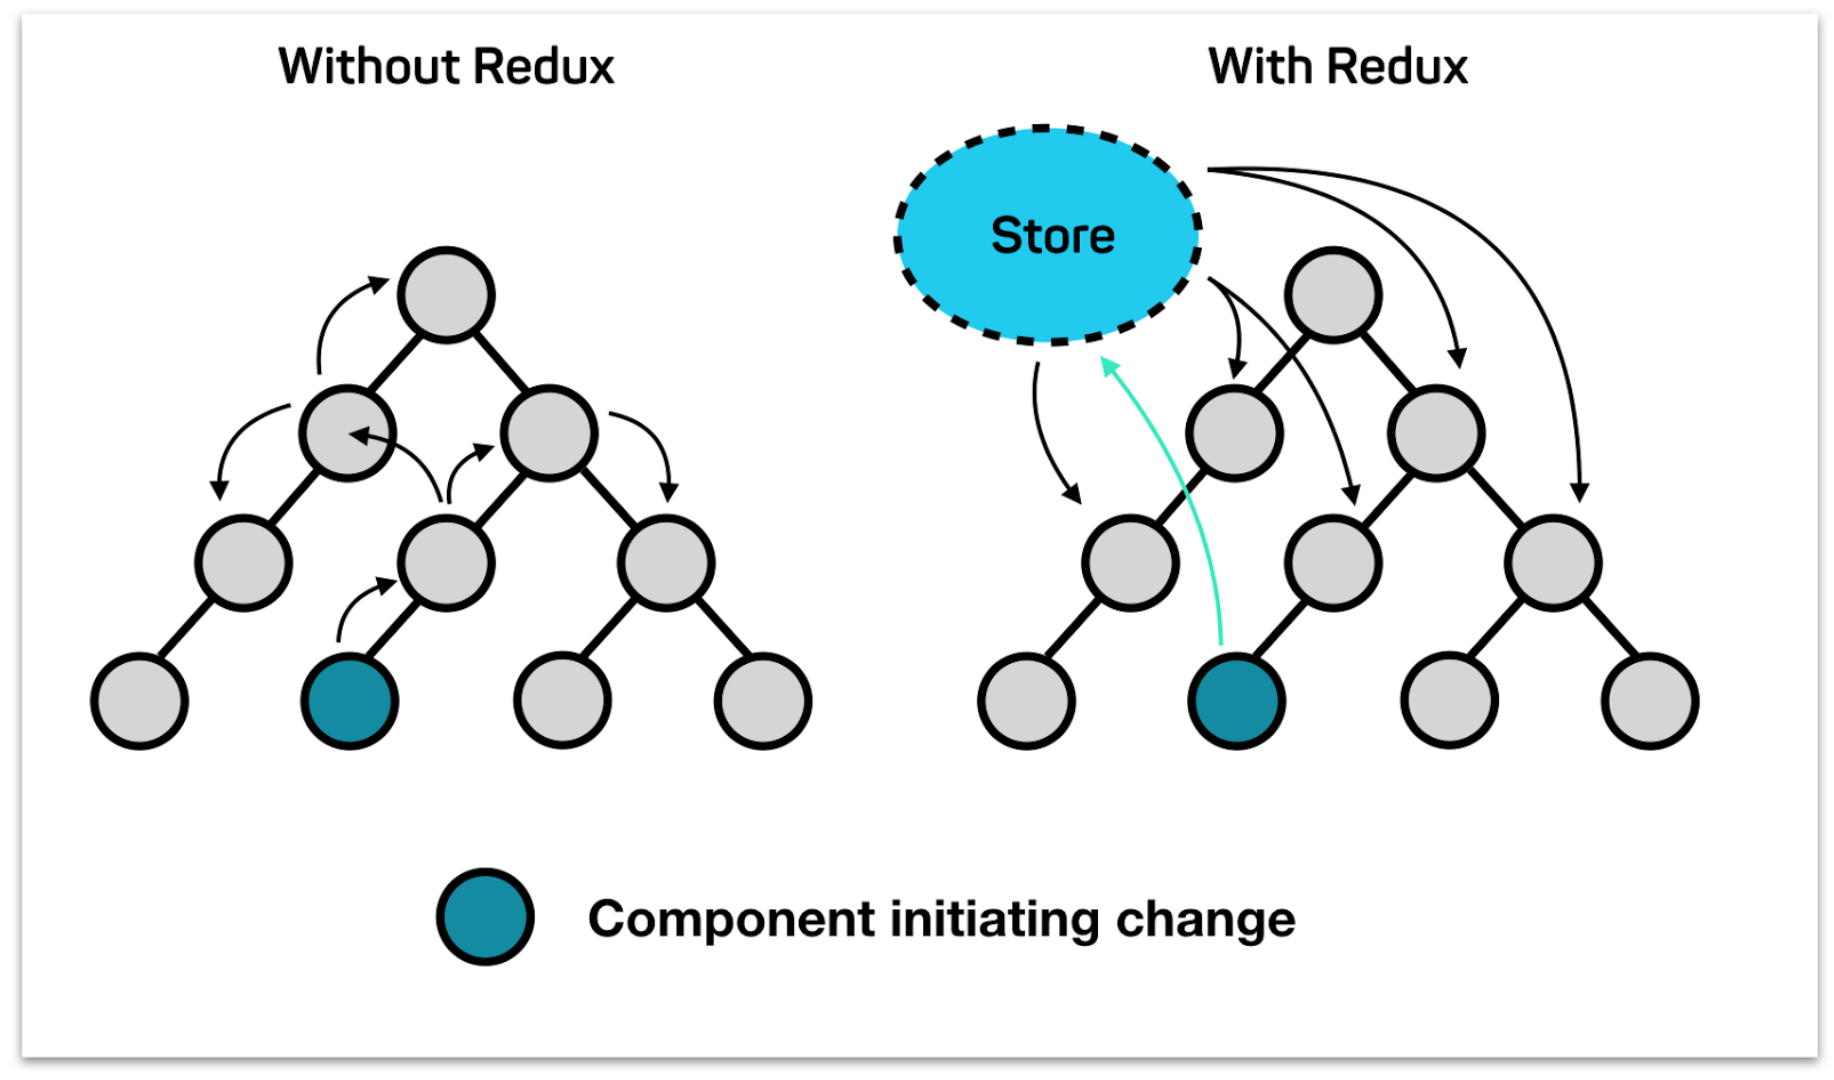
\includegraphics[width=12cm]{Image/Technical/redux.png}
        \caption{Quản lí state với Redux}
        \label{redux}
    \end{center}
\end{figure}
Các thành phần chính của Redux:
\begin{itemize}
    \item Store: là nơi lưu trữ của tất cả state trong ứng dụng, ta có thể truy cập vào để đọc, cập nhật và xóa các state thông qua các actions.
    \item Action: là các sự kiện mà người dùng tạo ra khi tác động vào các view để làm thay đổi state.
    \item Reducer: là một hàm nhận đầu vào là state và các mô tả về sự kiện và dựa vào đó để trả về state mới.
\end{itemize}

Cơ chế hoạt động của Redux (Hình \ref{redux-flow}):
\begin{enumerate}
    \item Ở component xảy ra một sự kiện nào đó của người dùng như nhấn vào một nút, nhấn vào phần tử, tạo hoặc xóa dữ liệu,...
    \item Action nhận được sự kiện trên component và thực hiện tạo một action gồm có kiểu và dữ liệu.
    \item Action này sẽ được gửi đến Reducer thông qua hàm dispatch(action), Reducer sẽ dựa và kiểu của action để lấy các dữ liệu ra tính toán và cập nhật lại dữ liệu của state đó.
    \item Sau khi state này thay đổi, component chứa nó sẽ thực hiện rerender lại.
\end{enumerate}

\begin{figure}[H]
    \begin{center}
        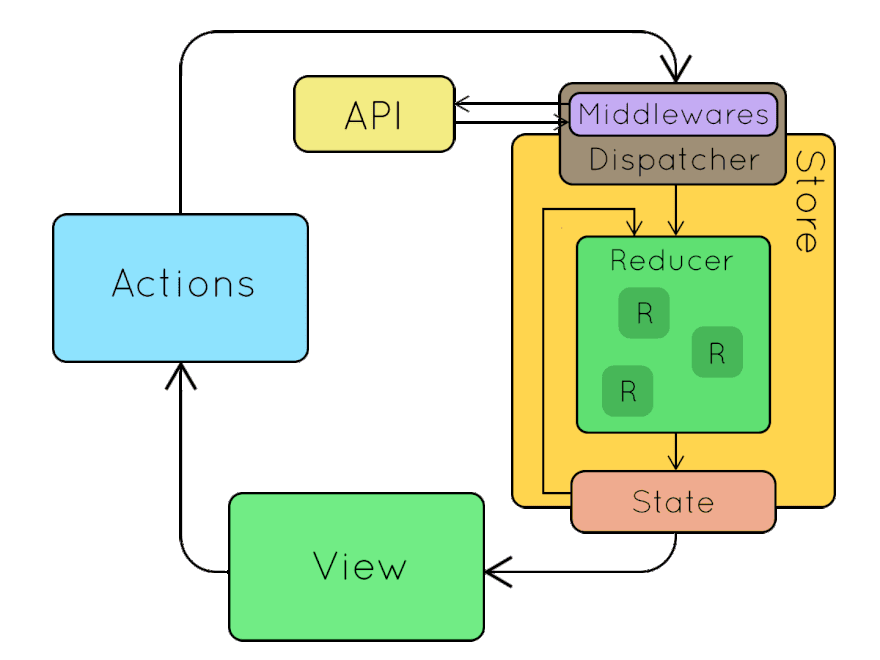
\includegraphics[width=12cm]{Image/Technical/redux-flow.png}
        \caption{Cơ chế hoạt động của Redux}
        \label{redux-flow}
    \end{center}
\end{figure}

\subsubsection{Tích hợp middleware sử dụng Redux Thunk}

Middleware là một lớp nằm giữa Reducer và Dispatch Actions, nó hoạt động sau khi một action được dispatch và trước khi reducer nhận được action này. Middleware trong redux được sử dụng nhiều nhất trong việc xử lí async action - những action không sẵn sàng khi người dùng dispatch, thông thường thì đây là các API request.\par

Hiện nay, có khá nhiều thư viện Middleware cho redux như redux-thunk, redux-saga, redux-observable,... Mỗi thư viện có những phương pháp giải quyết vấn đề riêng, tuy nhiên do thời gian thực hiện luận văn có hạn nên nhóm chọn redux-thunk, thư viện được giới thiệu bởi redux và đơn giản khi hiện thực, làm middleware cho hệ thống của mình.

\subsubsection{Xây dựng ứng dụng với framework Material-UI}

Một ứng dụng ReactJS được xây dựng bằng việc kết hợp các component lại với nhau. Ta có thể xây dựng các component cho ứng dụng bằng cách viết các component sau đó chỉnh sửa CSS từng chút một cho nó. Hiện nay, có khá nhiều thư viện phổ biến cung cấp cho ta các component cơ bản để phát triển giao diện như Boostrap, Material-UI, Ant Design,... Mỗi thư viện trên có các thiết kế theo các chuẩn khác nhau, nhóm đã xem qua và chọn Material-UI vì sự phổ biến, thiết kế đẹp và dễ dàng tùy chỉnh lại các style component một cách dễ dàng.\par


\subsection{Các công nghệ Server Side (Backend)}
Các ứng dụng web giống như những tảng băng trôi. Có một phần của ứng dụng mà người dùng nhìn thấy, tuy nhiên thì phần lớn nhất của ứng dụng vẫn là cái không nhìn thấy được - Backend. Nhiều công nghệ lập trình phía máy chủ đã ra đời và mỗi thứ đều có ưu điểm riêng. Mục tiêu của các công nghệ đó không chỉ giúp cho server chạy nhanh hơn mà còn đem lại trải nghiệm tốt hơn cho lập trình viên, giúp lập trình viên quản lý mã nguồn dễ hơn, debug dễ hơn, dễ tích hợp thêm tính năng mới hơn.
\subsubsection{Spring}
Spring là framework phát triển ứng dụng phổ biến nhất dành cho Java Enterprise. Spring có kích thướng nhẹ, phiên bản cơ bản của Spring framework có kích thước khoảng 2MB. Với Spring Framework các nhà phát triển có thể tạo ra các mã có hiệu suất cao, dễ kiểm thử và có thể sử dụng lại được.\par
Các tính năng core của Spring Framework có thể được sử dụng trong việc phát triển bất kỳ ứng dụng Java nào. Bên cạnh đó, phần mở rộng được sử dụng để xây dựng các ứng dụng web trên nền tảng Java EE. Mục tiêu của Spring Framework là làm cho việc phát triển ứng dụng J2EE dễ dàng hơn và thúc đẩy việc lập trình tốt hơn bằng mô hình POJO-based.
\begin{figure}[h!]
    \begin{center}
        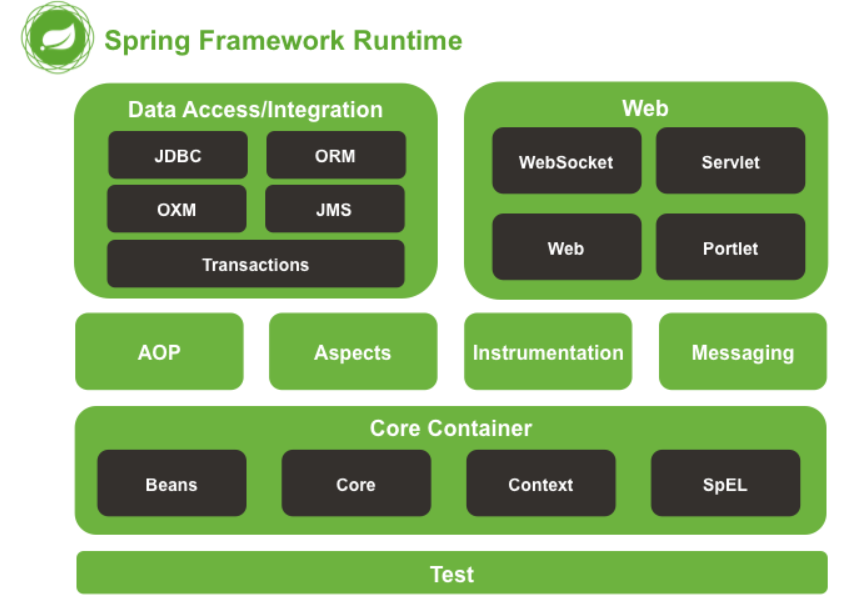
\includegraphics[width=10.8cm]{Image/Technical/spring_framework.png}
        \caption{Spring Framework}
        \label{spring}
    \end{center}
\end{figure}
\\
Ưu điểm của việc sử dụng Spring Framework:
\begin{itemize}
    \item Spring cho phép các nhà phát triển tạo các ứng dụng cấp Enterprise sử dụng các POJO. 
    \item Spring được tổ chức theo kiểu mô đun, dễ quản lí và phát triển.
    \item Dễ dàng để kiểm thử một chương trình được viết bằng Spring.
    \item Web framework của Spring là một Web MVC framework có thiết kế tốt, nó là một thay thế tuyệt vời cho Struts và các công nghệ kém phổ biến khác.
    \item IoC Container của Spring có trọng lượng nhẹ.
    \item Spring cung cấp một giao diện quản lý transaction nhất quán có thể mở rộng đến một local transaction.
\end{itemize}
Nhược điểm:
\begin{itemize}
    \item Không có một hệ sinh thái thư viện mạnh mẽ như các framework khác.
    \item Khó tiếp cận đối với người mới học lập trình web.
\end{itemize}

\subsubsection{Hibernate Framework}
Cơ sở dữ liệu quan hệ hướng đối tượng (Object-relational Database - ORD) là một hệ thống quản lý cơ sở dữ liệu (DBMS) bao gồm cả cơ sở dữ liệu quan hệ (RDBMS) và cơ sở dữ liệu hướng đối tượng (OODBMS). Cơ sở dữ liệu quan hệ đối tượng hoạt động như một giao diện giữa cơ sở dữ liệu quan hệ và hướng đối tượng vì nó chứa các khía cạnh và đặc điểm từ cả hai mô hình.\par

Cơ sở dữ liệu quan hệ hướng đối tượng (ORD) phục vụ hai mục đích chính:
\begin{itemize}
    \item Kết nối sự phân chia giữa cơ sở dữ liệu quan hệ và các kỹ thuật mô hình hướng đối tượng thường được sử dụng trong các ngôn ngữ lập trình như C\#, Java và C ++.
    \item Thu hẹp khoảng cách giữa các kỹ thuật mô hình hóa dữ liệu khái niệm cho cơ sở dữ liệu quan hệ và hướng đối tượng như sơ đồ entry-relationship (ERD) và ánh xạ quan hệ đối tượng (ORM).
\end{itemize}

Cơ sở dữ liệu hướng đối tượng (Object Oriented Database - OOD) được tổ chức xung quanh các đối tượng hơn là quan hệ, dữ liệu hơn là logic. Do đó, OOD là một hệ quản trị cơ sở dữ liệu trong đó thông tin được biểu diễn dưới dạng các đối tượng như được sử dụng trong lập trình hướng đối tượng (object).\par

Thông thường, khi OODBMS được tích hợp với một ngôn ngữ lập trình hướng đối tượng, sẽ nhất quán hơn nhiều giữa cơ sở dữ liệu và ngôn ngữ lập trình vì cả hai đều sử dụng cùng một mô hình biểu diễn dữ liệu. Khi so sánh với cơ sở dữ liệu quan hệ, cơ sở dữ liệu hướng đối tượng lưu trữ dữ liệu phức tạp, mối quan hệ giữa các dữ liệu trực tiếp mà không cần ánh xạ tới các hàng và cột như trong khi cơ sở dữ liệu quan hệ.\par

Sự khác nhau của Cơ sở dữ liệu hướng đối tượng (Object Oriented Database) và Cơ sở dữ liệu hướng quan hệ (Object Relational Database):\\

\begin{table}[h]
    \centering
    \begin{tabular}{|m{3cm}|m{5cm}|m{5cm}|}
    \hline 
        \textbf{Cơ sở so sánh} & \textbf{Object Oriented Database} & \textbf{Object Relational Database}\\ \hline
        Kết nối giữa hai quan hệ 
        & Các mối quan hệ được thể hiện bằng các tham chiếu thông qua mã định danh đối tượng (id).
        & Các kết nối giữa hai quan hệ được biểu diễn bằng các thuộc tính khóa ngoại trong một quan hệ tham chiếu đến khóa chính của một quan hệ khác.\\ \hline
        Cấu trúc lưu trữ dữ liệu 
        & Sử dụng các kỹ thuật lập chỉ mục để định vị các trang đĩa lưu trữ đối tượng. Do đó, chúng có thể cung cấp khả năng lưu trữ liên tục cho các đối tượng có cấu trúc phức tạp. 
        & Không chỉ định bất kỳ cấu trúc lưu trữ dữ liệu nào, mỗi quan hệ cơ sở được triển khai dưới dạng tệp riêng biệt và do đó, chúng không thể cung cấp khả năng lưu trữ liên tục cho các đối tượng có cấu trúc phức tạp.\\ \hline
        Số lượng dữ liệu 
        & Xử lý dữ liệu lớn hơn và phức tạp hơn.
        & Xử lý dữ liệu tương đối đơn giản hơn.\\ \hline
        Các ràng buộc 
        & Các ràng buộc được hỗ trợ bởi khác nhau với các hệ thống khác nhau. 
        & Nó có các khóa, tính toàn vẹn của thực thể và tính toàn vẹn của tham chiếu.\\ \hline
        Ngôn ngữ thao tác dữ liệu 
        & Thường được kết hợp với một ngôn ngữ lập trình như Java, C\#,... 
        & Có các ngôn ngữ thao tác dữ liệu như SQL, QUEL và QBE dựa trên quan hệ.\\ \hline
        Kiểu dữ liệu 
        & Có thể xử lý các loại dữ liệu khác nhau.
        & Có thể xử lý một kiểu dữ liệu duy nhất.\\ \hline
        Lưu trữ dữ liệu 
        & Dữ liệu được lưu trữ dưới dạng các đối tượng.
        & Dữ liệu được lưu trữ dưới dạng bảng, chứa các hàng và cột.\\
    \hline 
    \end{tabular}
    \caption{Object Oriented Database và Object Relational Database.}
    \label{OOD and ORD}
\end{table}

ORM (Object Relational Mapping) giúp đơn giản hoá việc tạo ra dữ liệu, thao tác dữ liệu và truy cập dữ liệu. Đó là một kỹ thuật lập trình để ánh xạ đối tượng vào dữ liệu được lưu trữ trong cơ sở dữ liệu. Hibernate framework là một giải pháp ORM mã nguồn mở, gọn nhẹ. Hibernate giúp đơn giản hoá sự phát triển của ứng dụng java để tương tác với cơ sở dữ liệu.\\
 \begin{figure}[h!]
    \begin{center}
        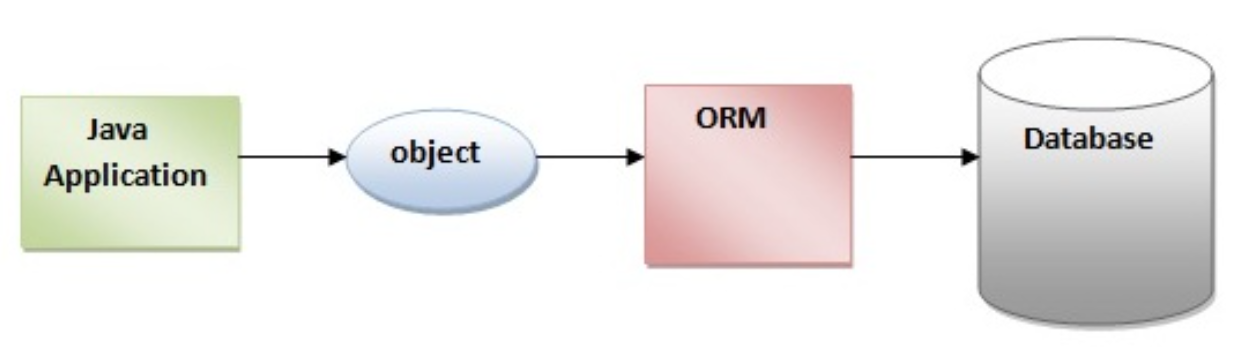
\includegraphics[width=15cm]{Image/Technical/hibernate_module.png}
        \caption{Mô hình Hibernate}
        \label{spring}
    \end{center}
\end{figure}

Hibernate Framework có các ưu điểm như dưới đây:
\begin{itemize}
    \item Mã nguồn mở và nhẹ.
    \item Hiệu suất nhanh.
    \item Truy vấn cơ sở dữ liệu độc lập.
    \item Tạo bảng tự động.
    \item Đơn giản lệnh join phức tạp.
    \item Cung cấp thống kê truy vấn và trạng thái cơ sở dữ liệu.
\end{itemize}
Bên cạnh đó Hibernate Framework ccũng có các nhược điểm:
\begin{itemize}
    \item Không hỗ trợ các câu truy vấn phức tạp.
    \item Một số trường hợp vẫn phải dùng native SQL do Hibernate không thể cover hết tất cả các cú pháp của các hệ quản trị cơ sử dữ liệu.
    \item Bị hạn chế sự can thiệp vào câu lệnh SQL do nó được tự động sinh ra.
\end{itemize}

\subsubsection{JPA Query Language}
JPA (Java Persistence API) thực hiện nhiệm vụ ánh xạ giữa các đối tượng Java với cơ sở dữ liệu quan hệ, sử dụng ORM (Object Relational Mapping).\par

JPA hoạt động như một cầu nối giữa các quan hệ trong database với các đối tượng Java, có thể persist một đối tượng Java vào trong cơ sở dữ liệu hoặc lấy dữ liệu từ cơ sở dữ liệu và ánh xạ ra các đối tượng Java. Các công cụ của JPA cho phép chúng ta thực hiện điều đó một cách đơn giản và nhanh chóng.\par

Spring Boot JPA là một phần trong hệ sinh thái Spring Data, nó tạo ra một layer ở giữa tầng service và database, giúp chúng ta thao tác với database một cách dễ dàng hơn, tự động config và giảm thiểu code thừa thãi.\par

Khi sử dụng JPA, chúng ta có thế:
\begin{itemize}
    \item Viết ít code hơn, nhưng vẫn có được performance tốt.
    \item Độc lập về database, không phải làm việc trực tiếp với các quan hệ.
\end{itemize}

\subsection{Cơ sở dữ liệu}
PostgreSQL là một hệ quản trị cơ sở dữ liệu quan hệ với mã nguồn mở mạnh mẽ, sử dụng và mở rộng ngôn ngữ SQL, kết hợp với nhiều tính năng giúp lưu trữ và xử lí khối dữ liệu hiệu quả nhất. PostgreSQL ra đời năm 1986 như một phần của dự án POSTGRES tại Đại học California (Berkeley) và đã có hơn 30 năm phát triển tích cực trên nền tảng cốt lõi.\par

PostgreSQL đã tạo được danh tiếng mạnh mẽ nhờ kiến trúc, độ tin cậy, tính toàn vẹn của dữ liệu, bộ tính năng mạnh mẽ, khả năng mở rộng và sự đóng góp của cộng đồng mã nguồn mở đằng sau để liên tục cung cấp các giải pháp hiệu quả và sáng tạo. PostgreSQL chạy trên tất cả các hệ điều hành chính, tuân thủ ACID từ năm 2001 và có các tiện ích bổ sung mạnh mẽ như bộ mở rộng cơ sở dữ liệu không gian địa lý PostGIS. Không có gì ngạc nhiên khi PostgreSQL đã trở thành hệ quản trị cơ sở dữ liệu mã nguồn mở được nhiều người và tổ chức lựa chọn.\par

 \begin{figure}[H]
    \begin{center}
        
\includegraphics[width=12cm]{Image/Technical/postgresql.png}
        \caption{Postgres Database.}
        \label{postgres}
    \end{center}
\end{figure}

\par
Postgres SQL có những ưu điểm như dưới đây:
\begin{itemize}
    \item Mã nguồn mở và nhẹ.
    \item Dễ sử dụng, sửa đổi và triển khai.
    \item Có khả năng chịu lỗi cao nhờ vào cơ chế ghi nhật kí trước (write-ahead logging - WAL)
    \item Hỗ trợ các đối tượng địa lý để có thể sử dụng nó cho các dịch vụ dựa trên vị trí và hệ thống thông tin địa lý.
    \item Cộng đồng sử dụng lớn mạnh.
\end{itemize}
Bên cạnh đó Postgres SQL ccũng có các nhược điểm:
\begin{itemize}
    \item Hiệu suất thực hiện các toán tử đơn giản kém hơn so với các hệ quản trị cơ sở dữ liệu quan hệ khác như MySQL, Oracle,... Nhưng đối với toán tử phức tạp thì tốt hơn rất nhiều.
    \item Do vẫn còn là một hệ quản trị cơ sở dữ liệu mới nên vẫn chưa được hỗ trợ một cách đầy đủ nhất.
\end{itemize}



%%%%%%%%%%%%%%%%%%%%%%%%%%%%%%%%%
\newpage
\section{Phân tích yêu cầu}

\subsection{Chức năng của hệ thống}
Xây dựng một hệ thống quản lý quá trình gia công nhuộm cho một doanh nghiệp vải sợ trên nền web, đáp ứng tối thiểu được những chức năng cơ bản để quản lý, đồng thời đảm bảo việc quản lý người dùng của quản trị viên.
\subsubsection{Đối với người dùng là nhân viên}
\begin{itemize}
    \item Quản lí tài khoản cá nhân.
    \begin{itemize}
        \item Đăng nhập.
        \item Đăng xuất.
        \item Khôi phục mật khẩu.
    \end{itemize}
    \item Quản lí xưởng nhuộm.
    \begin{itemize}
        \item Xem danh sách các xưởng, tìm kiếm và sắp xếp các xưởng.
        \item Xem thông tin chi tiết của xưởng
        \item Chỉnh sửa thông tin cơ bản của xưởng.
        \item Xem công nợ của xưởng.
        \item Tạo thanh toán cho xưởng.
    \end{itemize}
    \item Quản lí đơn đặt hàng.
    \begin{itemize}
        \item Tạo đơn đặt hàng từ trang chủ hoặc từ xưởng cụ thể.
        \item Xem danh sách đơn đặt hàng từ trang chủ hoặc từ xưởng cụ thế, có thể lọc và sắp xếp danh sách.
        \item Xem thông tin chi tiết của đơn đặt hàng.
    \end{itemize}
    \item Quản lí vải mộc.
    \begin{itemize}
        \item Xuất vải mộc cho các xưởng.
        \item Xem số lượng vải mộc tồn ở kho và các xưởng.
    \end{itemize}
    \item Quản lí vải thành phẩm.
    \begin{itemize}
        \item Nhập vải thành phẩm từ xưởng nhuộm.
        \item Xem danh sách lô nhuộm, có thể lọc theo lô, theo loại vải và theo màu sắc.
        \item Xem thông tin chi tiết của từng lô nhuộm.
    \end{itemize}
    \item Quản lí hàng trả.
    \begin{itemize}
        \item Xem danh sách phiếu hàng trả.
        \item Xem chi tiết phiếu hàng trả.
        \item Tạo phiếu hàng trả.
    \end{itemize}
\end{itemize}
\subsubsection{Đối với người dùng là quản trị viên}
\begin{itemize}
    \item Tạo mới tài khoản cho nhân viên.
    \item Tạo mới xưởng nhuộm.
\end{itemize}


\subsection{Yêu cầu phi chức năng của hệ thống}
\begin{itemize}
    \item Bảo mật.
    \begin{itemize}
        \item Phân quyền đăng nhập, truy cập hệ thống: người dùng - quản trị viên.
        \item Sử dụng thuật toán băm bảo mật SHA-256 để lưu trữ mật khẩu.
        \item Các mức Create, Read, Update, and Delete (CRUD).
        \item Kiểm tra persistent bằng hash token.
        \item Giới hạn thời gian giữ phiên đăng nhập hệ thống.
    \end{itemize}
    \item Hiệu năng.
    \begin{itemize}
        \item Thời gian tải trang, làm mới trình duyệt không vượt quá 5 giây.
        \item Thời gian xử lý - chức năng, tính toán không vượt quá 2 giây.
    \end{itemize}
    \item UI/UX
    \begin{itemize}
        \item Giao diện dễ nhìn, dễ sử dụng.
        \item Khả năng tương tác tốt.
    \end{itemize}
    \item Tính khả dụng:  
    \begin{itemize}
        \item Thời gian hoạt động: luôn hoạt động.
        \item Thời gian bảo trì: ngày lễ, nâng cấp hệ thống,...
    \end{itemize}
\end{itemize}

\subsection{Usecase}
\subsubsection{Lược đồ Usecase}
Đối tượng thao tác trên hệ thống gồm có: Nhân viên và quản trị viên.\par
Các chức năng được đặc tả trong sơ đồ Usecase như Hình \ref{usecase} dưới đây.
\newpage
\begin{figure}[h!]
    \begin{center}
        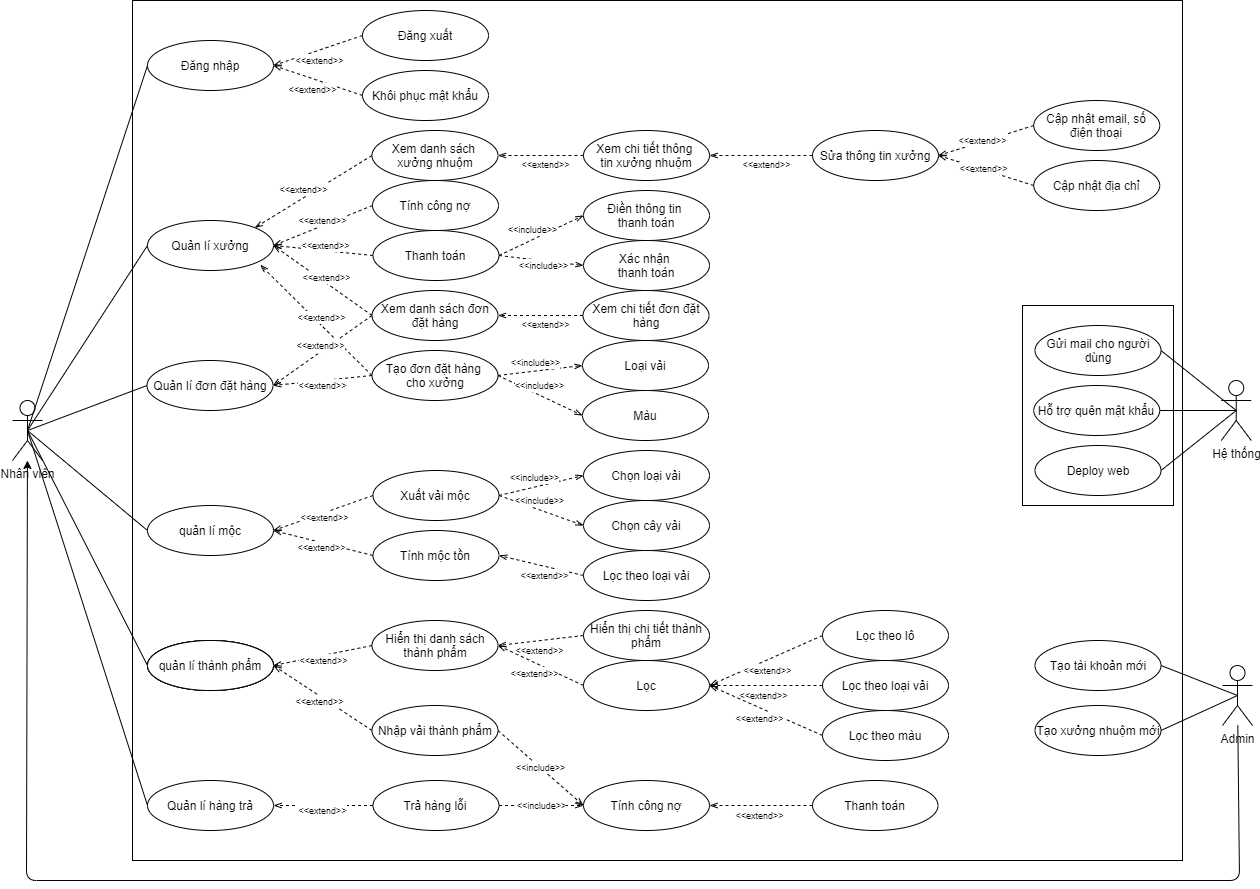
\includegraphics[width=16cm]{Image/General/Usecase.png}
        \caption{Usecase}
        \label{usecase}
    \end{center}
\end{figure}

\newpage
\subsubsection{Đặt tả Usecase}
\textbf{Đăng nhập}\par
\textbf{User story:} Là một người dùng của hệ thống, tôi muốn mình có thể đăng nhập vào để sử dụng hệ thống. Thông tin đăng nhập gồm có email và mật khẩu. Nếu tôi chưa đăng nhập, và cố gắng truy cập vào các trang của hệ thống, hệ thống sẽ chuyển hướng về trang đăng nhập. Nếu như quá 30 phút mà tôi không có hành động gì với hệ thống, thì phiên đăng nhập hết hạn và khi đó tôi sẽ phải đăng nhập lại. [\ref{bang1}]
\begin{table}[!htp]
    \centering
    \begin{tabular}{|m{3cm}|m{10cm}|}
    \hline 
        Use-case ID & 1\\ \hline
        Use-case name & Đăng nhập\\ \hline
        Actor & Nhân viên, quản trị viên.\\ \hline
        Description & Người dùng phải nhập tài khoản, mật khẩu để có thể sử dụng hệ thống.\\ \hline
        Preconditions & Người dùng đã đăng kí tài khoản và đang ở trang đăng nhập.\\ \hline
        Postconditions & Người dùng đã đăng nhập và có thể sử dụng hệ thống.\\ \hline
        Normal Flow & 
        1. Nhập tài khoản người dùng, hoặc email mà người dùng đã đăng kí cho tài khoản.\par
        2. Nhập mật khẩu.\par
        3. Bấm vào nút "Đăng nhập".
        \\ \hline
        Exception & 
        3a. Người dùng nhập tài khoản không chính xác.\par
        3b. Người dùng nhập mật khẩu không chính xác
        \\ \hline
        Alternative flow & Không có\\ 
    \hline 
    \end{tabular}
    \caption{Đăng nhập.}
    \label{bang1}
\end{table}

\newpage
\textbf{Khôi phục mật khẩu}\par
\textbf{User story:} Là một người dùng của hệ thống, tôi muốn có thể khôi phục lại mật khẩu của mình trong trường hợp quên mật khẩu hoặc muốn cập nhật mật khẩu mới. Khi yêu cầu khôi phục mật khẩu, tôi sẽ phải cung cấp email của mình, sau đó một email sẽ được hệ thống gửi đến chưa một đường dẫn, khi nhấn vào đường dẫn tôi sẽ được chuyển đến trang nhập mật khẩu mới. Thời gian hết hạn của đường dẫn trong mail trên là 5 phút, khi đó tôi phải thực hiện lại yêu cầu khôi phục mật khẩu. [\ref{bang2}]
\begin{table}[!htp]
    \centering
    \begin{tabular}{|m{3cm}|m{10cm}|}
    \hline 
        Use-case ID & 2\\ \hline
        Use-case name & Khôi phục mật khẩu.\\ \hline
        Actor & Nhân viên, quản trị viên.\\ \hline
        Description & Người dùng quên mật khẩu tài khoản của mình thì vẫn có thể đặt lại mật khẩu mới qua xác thực email.\\ \hline
        Preconditions & Người dùng đã có tài khoản hệ thống.\\ \hline
        Postconditions & Người dùng đặt lại mật khẩu mới.\\ \hline
        Normal Flow & 
        1. Nhấn vào Quên mật khẩu trên trang đăng nhập.\par
        2. Nhập email đã đăng kí cho tài khoản.\par
        3. Hệ thống sẽ gửi email, trên email sẽ có đường link để đổi mật khẩu, nhấn vào link.\par
        4. Nhập mật khẩu mới.\par
        5. Nhấn xác nhận.
        \\ \hline
        Exception & 3a. Nếu không thấy email thì tài khoản này không tồn tại.\\ \hline
        Alternative flow & Không có.\\ 
    \hline 
    \end{tabular}
    \caption{Khôi phục mật khẩu.}
    \label{bang2}
\end{table}

\newpage
\textbf{Dashboard}\par
\textbf{User story:} Là người dùng của hệ thống, tôi có thể xem một số thông tin thống kê về hoạt động của công ty gần đây. Sau khi đăng nhập thành công, tôi sẽ được chuyển đến trang Dashboard, ở đây tôi có thể xem thống kê về số lượng vải thành phẩm mà các xưởng nhuộm đã làm được trong vòng một năm qua, số tiền mà công ty đã thanh toán cho các xưởng nhuộm trong tuần qua, thống kế phần trăm lượng vải thành phẩm mà các xưởng đã làm cho công ty, các phiếu nhập và phiếu xuất gần đây của công ty. [\ref{bang14}]
\begin{table}[!htp]
    \centering
    \begin{tabular}{|m{3cm}|m{10cm}|}
    \hline 
        Use-case ID & 14\\ \hline
        Use-case name & Dashboard\\ \hline
        Actor & Nhân viên, quản trị viên.\\ \hline
        Description & Người dùng có thể xem các thông tin thống kê.\\ \hline
        Preconditions & Người dùng đã đăng nhập vào hệ thống.\\ \hline
        Postconditions & Người dùng xem các thông tin thống kê.\\ \hline
        Normal Flow & 
        1. Thống kê sản lượng trong năm gần đây của từng xưởng nhuộm.\par
        2. Thống kê vải thành phẩm theo xưởng và Thống kê vải thành phẩm theo loại vải.\par
        3. Danh sách phiếu nhập gần đây.\par
        4. Danh sách phiếu xuất gần đây.
        \\ \hline
        Exception & Khống có.\\ \hline
        Alternative flow & Không có.\\ 
    \hline 
    \end{tabular}
    \caption{Dashboard}
    \label{bang14}
\end{table}

\newpage
\textbf{Tạo nhân viên mới}\par
\textbf{User story:} Là người dùng của hệ thống, với vai trò là người quản trị hệ thống, tôi có thể tạo một nhân viên mới để truy cập vào hệ thống này. Khi nhấn vào Tạo nhân viên trên menu, tôi sẽ được chuyển sang trang tạo nhân viên mới. Ở đây, tôi cung cấp các thông tin họ, tên, email, mật khẩu, giới tính của nhân viên. Cuối cùng nhấn nút tạo nhân viên. Chức năng này không khả dụng nếu người dùng là nhân viên bình thường. [\ref{bang15}]
\begin{table}[!htp]
    \centering
    \begin{tabular}{|m{3cm}|m{10cm}|}
    \hline 
        Use-case ID & 15\\ \hline
        Use-case name & Tạo nhân viên mới\\ \hline
        Actor & Quản trị viên.\\ \hline
        Description & Quản trị viên có thể tạo nhân viên mới.\\ \hline
        Preconditions & Quản trị viên đã đăng nhập vào hệ thống.\\ \hline
        Postconditions & Nhân viên mới được tạo.\\ \hline
        Normal Flow & 
        1. Nhấn vào nút "Tạo nhân viên" trên thanh menu.\par 
        2. Nhập họ tên nhân viên mới.\par
        3. Nhập email.\par
        4. Nhập mật khẩu.\par
        5. Nhập giới tính.\par
        6. Nhấn nút "Tạo".
        \\ \hline
        Exception & Không có.
        \\ \hline
        Alternative flow & 
        6a. Nhấn nút "Hủy bỏ" để hủy tạo nhân viên.
        \\ 
    \hline 
    \end{tabular}
    \caption{Tạo nhân viên}
    \label{bang15}
\end{table}

\newpage
\textbf{Tạo xưởng nhuộm mới}\par
\textbf{User story:} Là người dùng của hệ thống, với vai trò là người quản trị hệ thống, tôi có thể tạo một xưởng nhuộm mới. Khi nhấn vào Tạo xưởng nhuộm trên menu, tôi sẽ được chuyển sang trang tạo xưởng nhuộm mới. Ở đây, tôi cung cấp các thông tin tên xưởng, địa chỉ, điện thoại và email của xưởng. Cuối cùng nhấn nút Lưu lại. Chức năng này không khả dụng nếu người dùng là nhân viên bình thường. [\ref{bang16}]
\begin{table}[!htp]
    \centering
    \begin{tabular}{|m{3cm}|m{10cm}|}
    \hline 
        Use-case ID & 16\\ \hline
        Use-case name & Tạo xưởng nhuộm mới\\ \hline
        Actor & Quản trị viên.\\ \hline
        Description & Quản trị viên có thể tạo xưởng nhuộm mới.\\ \hline
        Preconditions & Quản trị viên đã đăng nhập vào hệ thống.\\ \hline
        Postconditions & Xưởng nhuộm mới được tạo.\\ \hline
        Normal Flow & 
        1. Nhấn vào nút "Tạo xưởng nhuộm" trên thanh menu.\par 
        2. Nhập tên xưởng.\par
        3. Nhập địa chỉ.\par
        4. Nhập số điện thoại.\par
        5. Nhập email.\par
        6. Nhấn nút "Tạo".
        \\ \hline
        Exception & Không có.
        \\ \hline
        Alternative flow & 
        6a. Nhấn nút "Hủy bỏ" để hủy tạo xưởng nhuộm.
        \\ 
    \hline 
    \end{tabular}
    \caption{Tạo xưởng nhuộm}
    \label{bang16}
\end{table}

\newpage
\textbf{Xem xưởng nhuộm}\par
\textbf{User story:} Là một người dùng của hệ thống, tôi có thể xem được danh sách các xưởng nhuộm đang làm việc với công ty mình. Thông tin mỗi xưởng nhuộm bao gồm Tên xưởng nhuộm, công nợ và số lượng vải mộc tồn kho ở xưởng. Khi nhấn vào một xưởng, tôi có thể xem thông tin chi tiết về xưởng nhuộm. Thông tin chi tiết của xưởng bao gồm: tên xưởng, địa chỉ, số điện thoại, email, công nợ, danh sách các đơn đặt hàng ở xưởng này. Ngoài ra, có thêm các nút chỉnh sửa thông tin, tạo đơn đặt hàng, tạo thanh toán và danh sách vải tồn, khi nhấn vào sẽ có các hành động tương ứng như tiêu đề. [\ref{bang3}]
\begin{table}[!htp]
    \centering
    \begin{tabular}{|m{3cm}|m{10cm}|}
    \hline 
        Use-case ID & 3\\ \hline
        Use-case name & Xem xưởng nhuộm.\\ \hline
        Actor & Nhân viên, quản trị viên.\\ \hline
        Description & Nhân viên có thể xem danh sách các xưởng nhuộm, bao gồm mã xưởng, tên xưởng, tổng công nợ và tổng độ dài mộc tồn. Nhân viên nhấn vào tên xưởng để xem thông tin chi tiết về xưởng.\\ \hline
        Preconditions & Người dùng đã đăng nhập vào hệ thống.\\ \hline
        Postconditions & Người dùng có thể xem các thông tin về xưởng nhuộm.\\ \hline
        Normal Flow & 
        1. Nhấn vào nút "Danh sách xưởng nhuộm" trên thanh menu, danh sách xưởng nhuộm xuất hiện.\par
        2. Nhấn vào tiêu đề trên mỗi cột để sắp xếp.\par
        3. Sử dụng bộ lọc để lọc thông tin.\par
        4. Nhấn vào xưởng nhuộm trong danh sách để chuyển sang trang Chi tiết xưởng nhuộm.\par
        \\ \hline
        Exception & Không có.\\ \hline
        Alternative flow & 
        Không có. \par
        \\ 
    \hline 
    \end{tabular}
    \caption{Xem xưởng nhuộm.}
    \label{bang3}
\end{table}

\newpage
\textbf{Chỉnh sửa thông tin xưởng nhuộm.}\par
\textbf{User story:} Là người dùng của hệ thống, tôi có thể chỉnh sửa các thông tin cơ bản của một xưởng nhuộm. Khi nhấn vào nút chỉnh sửa thông tin trong trang chi tiết xưởng nhuộm, tôi có thể sửa địa chỉ, số điện thoại và email của xưởng này. Sau khi cập nhật xong, tôi sẽ thấy thông tin mới trong trang chi tiết xưởng nhuộm. [\ref{bang4}]
\begin{table}[!htp]
    \centering
    \begin{tabular}{|m{3cm}|m{10cm}|}
    \hline 
        Use-case ID & 4\\ \hline
        Use-case name & Chỉnh sửa thông tin xưởng nhuộm.\\ \hline
        Actor & Nhân viên, quản trị viên.\\ \hline
        Description & Người dùng có thể chỉnh sửa một số thông tin cơ bản về xưởng nhuộm như địa chỉ, số điện thoại và email.\\ \hline
        Preconditions & Người dùng đã đăng nhập vào hệ thống.\\ \hline
        Postconditions & Thông tin về xưởng nhuộm sẽ được chỉnh sửa\\ \hline
        Normal Flow & 
        1. Trên trang thông tin chi tiết của xưởng, nhấm vào nút "Chỉnh sửa thông tin".\par
        2. Nhập địa chỉ, số điện thoại và email cần sửa.\par
        3. Nhấn nút "Lưu".
        \\ \hline
        Exception & 
        2a. Hệ thống sẽ hiển thị thông tin hiện tại của xưởng, người dùng chỉ cần chỉnh sửa thông tin nào cần thay đổi.
        2b. Người dùng nhập số điện thoại không đúng độ dài hoặc email sai định dạng, hệ thống sẽ báo lỗi.
        \\ \hline
        Alternative flow & 
        3a. Nhấn nút "Hủy bỏ" để hủy chỉnh sửa.
        \\ 
    \hline 
    \end{tabular}
    \caption{Chỉnh sửa thông tin xưởng nhuộm.}
    \label{bang4}
\end{table}

\newpage
\textbf{Thanh toán}\par
\textbf{User story:} Là người dùng của hệ thống, tôi có thể tạo hóa đơn thanh toán công nợ cho một xưởng nhuộm. Khi nhấn vào nút Tạo thanh toán trong trang chi tiết xưởng nhuộm, hoặc nhấn vào Tạo hóa đơn ở menu, tôi sẽ được chuyển qua trang tạo hóa đơn thanh toán.Ở đây, tôi nhập các thông tin gồm xưởng nhuộm, phương thức thanh toán, ngân hàng (nếu có), tổng số tiền, và nhân viên xác nhận thanh toán ở xưởng nhuộm. [\ref{bang5}]
\begin{table}[!htp]
    \centering
    \begin{tabular}{|m{3cm}|m{10cm}|}
    \hline 
        Use-case ID & 5\\ \hline
        Use-case name & Thanh toán\\ \hline
        Actor & Nhân viên, quản trị viên.\\ \hline
        Description & Người dùng có thể thanh toán tiền cho xưởng nhuộm.\\ \hline
        Preconditions & Người dùng đã đăng nhập vào hệ thống.\\ \hline
        Postconditions & Xưởng nhuộm được thanh toán.\\ \hline
        Normal Flow & 
        1. Trong trang chi tiết của xưởng nhuộm, nhấn vào nút "Tạo thanh toán", màn hình Tạo thanh toán xuất hiện.\par
        2. Chọn xưởng nhuộm, phương thức thanh toán, ngân hàng hoặc tên người nhận\par
        3. Nhập số tiền cần thanh toán\par
        4. Nhập tên nhân viên nhận.\par
        5. Nhấn nút "Tạo".
        \\ \hline
        Exception & 
        3a. Nhập số tiền thanh toán lớn hơn công nợ của xưởng, hệ thống sẽ báo lỗi.
        \\ \hline
        Alternative flow & 
        1a. Nhấn nút "Danh sách công nợ" trên thanh menu, danh sách công nợ xuất hiện, sau đó nhấn vào nút "Thanh toán" của xưởng cụ thể.\par
        4a. Nhất nút "Hủy bỏ" để hủy thanh toán.
        \\ 
    \hline 
    \end{tabular}
    \caption{Thanh toán cho xưởng nhuộm.}
    \label{bang5}
\end{table}

\newpage
\textbf{Xem đơn đặt hàng}\par
\textbf{User story:} Là người dùng của hệ thống, tôi có thể xem danh sách các đơn đặt hàng mà công ty đã đặt ở các xưởng. Khi nhấn vào mục Danh sách đơn đặt hàng ở menu, tôi sẽ xem được danh sách các đơn. Thông tin một đơn gồm có: tên xưởng, ngày đặt, loại vải, màu đặt, độ dài đặt hàng, số lượng vải thành phẩm đã nhận và trạng thái của đơn hàng. Khi nhấn vào một đơn hàng, tôi sẽ được chuyển qua trang Chi tiết đơn hàng. Ngoài những thông tin như ngoài danh sách ra, tôi có thể thấy được danh sách các phiếu nhập hàng của đơn hàng này. Ngoài ra, tôi còn có thể cập nhật trạng thái của đơn hàng này sang Hoàn thành khi thực tế đã nhận đủ lượng hàng. [\ref{bang6}]
\begin{table}[!htp]
    \centering
    \begin{tabular}{|m{3cm}|m{10cm}|}
    \hline 
        Use-case ID & 6\\ \hline
        Use-case name & Xem đơn đặt hàng.\\ \hline
        Actor & Nhân viên, quản trị viên.\\ \hline
        Description & Nhân viên có thể xem danh sách các đơn đặt hàng, bao gồm mã đơn, tên xưởng, ngày đặt, loại vải, màu, độ dài đặt, đã nhận, trạng thái. Nhân viên nhấn đơn đặt hàng để xem thông tin chi tiết về đơn.\\ \hline
        Preconditions & Người dùng đã đăng nhập vào hệ thống.\\ \hline
        Postconditions & Người dùng có thể xem các thông tin về đơn đặt hàng.\\ \hline
        Normal Flow & 
        1. Nhấn vào nút "Đơn đặt hàng" trên thanh menu, danh sách đơn đặt hàng xuất hiện.\par
        2. Nhấn vào tiêu đề trên mỗi cột để sắp xếp.\par
        3. Sử dụng bộ lọc để lọc thông tin.\par
        3. Nhấn vào mã đơn để chuyển tới màn hình chi tiết của đơn đặt hàng.
        \\ \hline
        Exception & Không có.\\ \hline
        Alternative flow & 
        3a. Nhấn vào mã đơn trong danh sách đơn đặt hàng của trang thông tin chi tiết về xưởng để chuyển tới màn hình chi tiết của đơn đặt hàng.
        \\ 
    \hline 
    \end{tabular}
    \caption{Xem đơn đặt hàng.}
    \label{bang6}
\end{table}

\newpage
\textbf{Tạo đơn đặt hàng}\par
\textbf{User story:} Là người dùng của hệ thống, tôi có thể tạo một đơn đặt hàng mới với xưởng nhuộm. Tôi có thể nhấn vào Tạo đơn ở menu hoặc trong trang Chi tiết xưởng nhuộm để chuyển qua trang tạo đơn đặt hàng. Để tạo một đơn đặt hàng, tôi cần phải chọn xưởng nhuộm, chọn loại vải, chọn màu sắc và nhập vào độ dài cần đặt. Sau khi đặt hàng thành công, tôi sẽ được chuyển sang trang danh sách đơn đặt hàng. [\ref{bang7}]
\begin{table}[!htp]
    \centering
    \begin{tabular}{|m{3cm}|m{10cm}|}
    \hline 
        Use-case ID & 7\\ \hline
        Use-case name & Tạo đơn đặt hàng.\\ \hline
        Actor & Nhân viên, quản trị viên.\\ \hline
        Description & Người dùng có thể tạo đơn đặt hàng nhuộm cho xưởng nhuộm.\\ \hline
        Preconditions & Người dùng đã đăng nhập vào hệ thống.\\ \hline
        Postconditions & Đơn đặt hàng mới được tạo\\ \hline
        Normal Flow & 
        1. Nhấn vào nút "Tạo đơn" trên thanh menu, màn hình tạo đơn đặt hàng sẽ xuất hiện.\par
        2. Chọn xưởng nhuộm, loại vải, màu.\par
        3. Nhập độ dài vải cần đặt.\par
        4. Nhấn nút "Tạo".
        \\ \hline
        Exception & \\ \hline
        Alternative flow & 
        1a. Nhấn vào nút "Tạo đơn đặt hàng" trên trang chi tiết của xưởng nhuộm.\par
        4a. Nhấn nút "Hủy bỏ" để hủy tạo đơn đặt hàng.
        \\ 
    \hline 
    \end{tabular}
    \caption{Tạo đơn đặt hàng.}
    \label{bang7}
\end{table}

\textbf{Xem vải mộc}\par
\textbf{User story:} Là người dùng của hệ thống, tôi có thể xem được danh sách số vải mộc tồn ở kho của công ty và ở từng xưởng nhuộm theo từng loại vải. [\ref{bang8}]
\begin{table}[!htp]
    \centering
    \begin{tabular}{|m{3cm}|m{10cm}|}
    \hline 
        Use-case ID & 8\\ \hline
        Use-case name & Xem vải mộc.\\ \hline
        Actor & Nhân viên, quản trị viên.\\ \hline
        Description & Người dùng có thể xem số lượng vải mộc tồn trong kho và mộc tồn tại xưởng. Mộc tồn được phân loại theo loại vải.\\ \hline
        Preconditions & Người dùng đã đăng nhập vào hệ thống.\\ \hline
        Postconditions & Người dùng có thể xem các thông tin về vải mộc tồn.\\ \hline
        Normal Flow & 
        1. Nhấn vào nút "Danh sách vải tồn" trên thanh menu, màn hình danh sách vải mộc xuất hiện.\par
        2. Xem vải mộc tại kho, chọn "Kho". Thống kê theo loại vải.\par
        3. Xem vải mộc tại xưởng, chọn "Xưởng". Thống kê theo xưởng và loại vải.
        \\ \hline
        Exception & Không có.\\ \hline
        Alternative flow & Không có.\\ 
    \hline 
    \end{tabular}
    \caption{Xem vải mộc.}
    \label{bang8}
\end{table}

\newpage
\textbf{Tạo phiếu xuất vải mộc}\par
\textbf{User story:} Là người dùng của hệ thống, tôi có thể tạo phiếu xuất vải mộc cho các xưởng. Khi nhấn vào Tạo phiếu xuất ở menu, tôi sẽ được chuyển đến trang tạo phiếu xuất. Để tạo được phiếu, tôi phải nhập thông tin xưởng nhuộm và chọn loại vải, sau đó sẽ có một danh sách các cây vải của loại vải này sẽ được tải về, và cuối cùng tôi sẽ chọn danh sách cây vải nào cần xuất. [\ref{bang9}]
\begin{table}[!htp]
    \centering
    \begin{tabular}{|m{3cm}|m{10cm}|}
    \hline 
        Use-case ID & 9\\ \hline
        Use-case name & Tạo phiếu xuất vải mộc\\ \hline
        Actor & Nhân viên, quản trị viên.\\ \hline
        Description & Người dùng tạo phiếu xuất vải mộc cho xưởng nhuộm, phiếu xuất gồm nhiều cây vải có thể nhiều thuộc loại vải khác nhau.\\ \hline
        Preconditions & Người dùng đã đăng nhập vào hệ thống.
        \\ \hline
        Postconditions & Xuất vải mộc cho xưởng nhuộm.\\ \hline
        Normal Flow & 
        1. Nhấn nút "Tạo phiếu xuất" trên thanh menu, trang tạo phiếu xuất vải mộc xuất hiện.\par
        2. Chọn xưởng nhuộm cần xuất.\par
        3. Nhập mã của từng cây vải, sau đó nhấn nút "Thêm", cây vải sẽ được thêm vào danh sách hiển thị ra màn hình.\par
        4. Nhấn nút "Tạo".
        \\ \hline
        Exception & Không có.
        \\ \hline
        Alternative flow & 
        4a. Có thể nhấn kí tự xóa để xóa cây vải ra khỏi danh sách nếu không muốn thêm vào phiếu xuất.\par
        4b. Nhấn nút "Hủy bỏ" để hủy phiếu xuất.
        \\ 
    \hline 
    \end{tabular}
    \caption{Tạo phiếu xuất vải mộc cho xưởng.}
    \label{bang9}
\end{table}

\newpage
\textbf{Xem phiếu nhập vải thành phẩm}\par
\textbf{User story:} Là người dùng của hệ thống, tôi có thể xem danh sách các phiếu nhập hàng thành phẩm từ các xưởng nhuộm. Khi nhấn vào Danh sách phiếu nhập ở menu, tôi sẽ xem được danh sách này. Trong đó, mỗi hàng trong danh sách là một phiếu, gồm có các thông tin xưởng nhuộm, ngày nhuộm, loại vải, màu vải và tổng thành phẩm. Khi nhấn vào một phiếu, tôi sẽ được chuyển sang trang Chi tiết phiếu nhập, ở đây ngoài các thông tin như ngoài danh sách, thì có thêm danh sách các cây vải nhập về và độ dài thành phẩm trong phiếu này. [\ref{bang10}]
\begin{table}[!htp]
    \centering
    \begin{tabular}{|m{3cm}|m{10cm}|}
    \hline 
        Use-case ID & 10\\ \hline
        Use-case name & Xem vải thành phẩm.\\ \hline
        Actor & Nhân viên, quản trị viên.\\ \hline
        Description & Người dùng có thế xem danh sách các phiếu nhập vải thành phẩm từ xưởng, bao gồm mã phiếu, tổng thành phẩm, loại vải, màu, ngày nhộm.\\ \hline
        Preconditions & Người dùng đã đăng nhập vào hệ thống.\\ \hline
        Postconditions & Người dùng có thể xem thông tin về lô nhuộm và các cây vải thành phẩm trong lô.\\ \hline
        Normal Flow & 
        1. Nhấn vào nút "Danh sách phiếu nhập" trên thanh menu, trang danh sách phiếu nhập sẽ xuất hiện.\par
        2. Nhấn vào tiêu đề trên mỗi cột để sắp xếp.\par
        3. Sử dụng bộ lọc để lọc thông tin.
        \\ \hline
        Exception & Không có.\\ \hline
        Alternative flow & Không có.\\ 
    \hline 
    \end{tabular}
    \caption{Xem vải thành phẩm.}
    \label{bang10}
\end{table}

\newpage
\textbf{Tạo phiếu nhập vải thành phẩm}\par
\textbf{User story:} Là người dùng của hệ thống, tôi có thể tạo phiếu nhập vải thành phẩm từ xưởng nhuộm gửi về. Khi nhấn vào Tạo phiếu nhập trong menu, tôi sẽ được chuyển đến trang tạo vải thành phẩm. Ở đây, tôi cung cấp các thông tin gồm tài xế giao hàng, xưởng nhuộm, loại vải, màu và đơn đặt hàng. Bước tiếp theo, tôi sẽ nhập danh sách các cây vải thành phẩm, thông tin một cây vải bao gồm mã cây vải và độ dài thành phẩm. Cuối cùng nhấn nút Tạo phiếu. [\ref{bang11}]
\begin{table}[!htp]
    \centering
    \begin{tabular}{|m{3cm}|m{10cm}|}
    \hline 
        Use-case ID & 12\\ \hline
        Use-case name & Tạo phiếu nhập vải thành phẩm.\\ \hline
        Actor & Nhân viên, quản trị viên.\\ \hline
        Description & Người dùng sẽ tạo phiếu nhập vải thành phẩm từ xưởng nhuộm về kho. Mỗi phiếu nhập sẽ bao gồm nhiều cây vải thành phẩm.\\ \hline
        Preconditions & Người dùng đã đăng nhập vào hệ thống \\ \hline
        Postconditions & Phiếu nhập vải thành phẩm sẽ được tạo.\\ \hline
        Normal Flow & 
        1. Nhấn vào nút "Tạo phiếu nhập" trên thanh menu, trang tạo phiếu nhập sẽ xuất hiện.\par
        2. Nhập xưởng nhuộm, loại vải, màu cho lô nhuộm.\par
        3. Nhập mã đơn đặt hàng tương ứng.\par
        4. Nhập tên người giao hàng.\par
        5. Nhấn nút "Tiếp theo".\par
        6. Nhập lần lượt mã cây vải và độ dài thành phẩm, sau đó nhấn nút "Thêm" để thêm cây vải vào lô nhuộm, danh sách cây vải của lô được hiển thị ra màn hình.\par
        4. Kiểm tra thông tin, nhấn nút "Tạo phiếu" để hoàn thành.
        \\ \hline
        Exception & Không có.
        \\ \hline
        Alternative flow & 
        6a. Nhấn vào kí tự xóa để xóa cây vải nêu không muốn thêm vào lô nhuộm nữa.
        \\ 
    \hline 
    \end{tabular}
    \caption{Tạo phiếu nhập vải thành phẩm từ xưởng nhuộm.}
    \label{bang11}
\end{table}

\newpage
\textbf{Xem hàng trả}\par
\textbf{User story:} Là người dùng của hệ thống, tôi có thể xem danh sách các phiếu hàng trả. Mỗi hàng trong danh sách này là một phiếu, bao gồm các thông tin xưởng nhuộm, tổng tiền, ngày tạo, và nhân viên tạo. Khi nhấn vào một hàng, tôi sẽ xem được thông tin chi tiết. Thông tin chi tiết của phiếu bao gồm các thông tin bên ngoài và có thêm danh sách các cây vải, thông tin trong một cây vải bao gồm mã cây vải, màu, loại, độ dài thành phẩm, độ dài trả, thành tiền và lí do trả hàng. Cuối cùng là tổng hợp lại tổng số cây, tổng độ dài trả và tổng tiền. [\ref{bang12}]
\begin{table}[!htp]
    \centering
    \begin{tabular}{|m{3cm}|m{10cm}|}
    \hline 
        Use-case ID & 12\\ \hline
        Use-case name & Xem hàng trả\\ \hline
        Actor & Nhân viên, quản trị viên.\\ \hline
        Description & Người dùng có thể xem danh sách phiếu hàng trả. Mỗi phiếu hàng trả có thể có nhiều hàng trả. Người dùng có thể xem thông tin chi tiết của phiếu hàng trả bao gồm danh sách hàng trả của phiếu.\\ \hline
        Preconditions & Người dùng đã đăng nhập vào hệ thống.\\ \hline
        Postconditions & Người dùng xem được thông tin của phiếu hàng trả và danh sách hàng trả của phiếu hàng trả.\\ \hline
        Normal Flow & 
        1. Nhấn vào nút "Danh sách hàng trả" trên thanh menu, trang danh sách hàng trả xuất hiện.\par
        2. Nhấn vào mã phiếu để chuyển sang trang chi tiết về phiếu hàng trả.
        \\ \hline
        Exception & Không có\\ \hline
        Alternative flow & Không có\\ 
    \hline 
    \end{tabular}
    \caption{Xem hàng trả.}
    \label{bang12}
\end{table}

\newpage
\textbf{Tạo phiếu hàng trả}\par
\textbf{User story:} Là người dùng của hệ thống, tôi có thể tạo phiếu hàng trả cho các xưởng. Khi nhấn vào Tạo phiếu hàng trả ở menu, tôi sẽ được chuyển sang trang tạo hàng trả. Ở đây, tôi nhập các thông tin gồm Nhân viên nhận, xưởng nhuộm. Sau đó nhập thông tin cho từng cây hàng trả, bao gồm: mã cây vải, độ dài trả và mô tả lỗi. Sau khi nhập xong thông tin của các cây vải, nhấn nút Tạo phiếu để tạo. [\ref{bang13}]
\begin{table}[!htp]
    \centering
    \begin{tabular}{|m{3cm}|m{10cm}|}
    \hline 
        Use-case ID & 13\\ \hline
        Use-case name & Tạo phiếu hàng trả\\ \hline
        Actor & Nhân viên, quản trị viên.\\ \hline
        Description & Người dùng có thể tạo phiếu hàng trả, sau đó hàng trả sẽ lần lượt được thêm vào phiếu hàng trả.\\ \hline
        Preconditions & Người dùng đã đăng nhập vào hệ thống.\\ \hline
        Postconditions & Phiếu hàng trả và hàng trả được tạo.\\ \hline
        Normal Flow & 
        1. Nhấn vào nút "Tạo phiếu hàng trả" trên thanh menu.\par 
        2. Nhập tên người nhận hàng trả.\par
        3. Chọn xưởng nhuộm.\par 
        4. Nhập mã cây vải, độ dài trả, lí do trả.\par
        5. Nhấn nút "Tạo".
        \\ \hline
        Exception & Không có.
        \\ \hline
        Alternative flow & 
        5a. Nhấn nút "Hủy bỏ" để hủy phiếu hàng trả.
        \\ 
    \hline 
    \end{tabular}
    \caption{Tạo phiếu hàng trả}
    \label{bang13}
\end{table}

% \newpage
\textbf{Danh sách công nợ}\par
\textbf{User story:} Là người dùng của hệ thống, tôi có thể xem được danh sách công nợ của các xưởng nhuộm. Mỗi hàng trong danh sách này là một xưởng nhuộm, số tiền nợ, và nút Thanh toán. Khi nhấn nút Thanh toán tôi sẽ được chuyển qua trang tạo thanh toán cho xưởng tương ứng. [\ref{bang17}]
\begin{table}[!htp]
    \centering
    \begin{tabular}{|m{3cm}|m{10cm}|}
    \hline 
        Use-case ID & 17\\ \hline
        Use-case name & Danh sách công nợ\\ \hline
        Actor & Nhân viên, quản trị viên.\\ \hline
        Description & Xem danh sách công nợ của các xưởng nhuộm.\\ \hline
        Preconditions & Người dùng đã đăng nhập vào hệ thống.\\ \hline
        Postconditions & Người dùng có thể xem các thông tin về công nợ.\\ \hline
        Normal Flow & 
        1. Nhấn vào nút "Danh sách công nợ" trên thanh menu, danh sách công nợ xuất hiện.
        \\ \hline
        Exception & Không có\\ \hline
        Alternative flow & Không có\\ 
    \hline 
    \end{tabular}
    \caption{Danh sách công nợ}
    \label{bang17}
\end{table}

\newpage
\textbf{Danh sách hoá đơn thanh toán}\par
\textbf{User story:} Là người dùng của hệ thống, tôi có thể xem được danh sách hoá đơn đã thanh toán cho các xưởng nhuộm. Mỗi hàng trong danh sách này là một hoá đơn bao gồm các thông tin xưởng nhuộm, số tiền, phương thức thanh toán, ngân hàng, ngày tạo, nhân viên tạo, nhân viên nhận. [\ref{bang18}]
\begin{table}[!htp]
    \centering
    \begin{tabular}{|m{3cm}|m{10cm}|}
    \hline 
        Use-case ID & 18\\ \hline
        Use-case name & Danh sách hoá đơn thanh toán\\ \hline
        Actor & Nhân viên, quản trị viên.\\ \hline
        Description & Xem danh sách hoá đơn thanh toán của các xưởng nhuộm.\\ \hline
        Preconditions & Người dùng đã đăng nhập vào hệ thống.\\ \hline
        Postconditions & Người dùng có thể xem các thông tin về hoá đơn thanh toán.\\ \hline
        Normal Flow & 
        1. Nhấn vào nút "Danh sách hoá đơn" trên thanh menu, danh sách hoá đơn xuất hiện.\par
        2. Nhấn vào tiêu đề trên mỗi cột để sắp xếp.\par
        3. Sử dụng bộ lọc để lọc thông tin.
        \\ \hline
        Exception & Không có\\ \hline
        Alternative flow & Không có\\ 
    \hline 
    \end{tabular}
    \caption{Danh sách hoá đơn thanh toán}
    \label{bang18}
\end{table}

% \textbf{User story:} [\ref{bang5}]
% \begin{table}[!htp]
%     \centering
%     \begin{tabular}{|m{3cm}|m{10cm}|}
%     \hline 
%         Use-case ID & 1\\ \hline
%         Use-case name & \\ \hline
%         Actor & \\ \hline
%         Description & \\ \hline
%         Preconditions & \\ \hline
%         Postconditions & \\ \hline
%         Normal Flow & \\ \hline
%         Exception & \\ \hline
%         Alternative flow & \\ 
%     \hline 
%     \end{tabular}
%     \caption{Đăng nhập}
%     \label{bang1}
% \end{table}





%%%%%%%%%%%%%%%%%%%%%%%%%%%%%%%%%
\newpage
\section{Thiết kế hệ thống}

\subsection{Kiến trúc hệ thống}
\begin{figure}[H]
    \begin{center}
        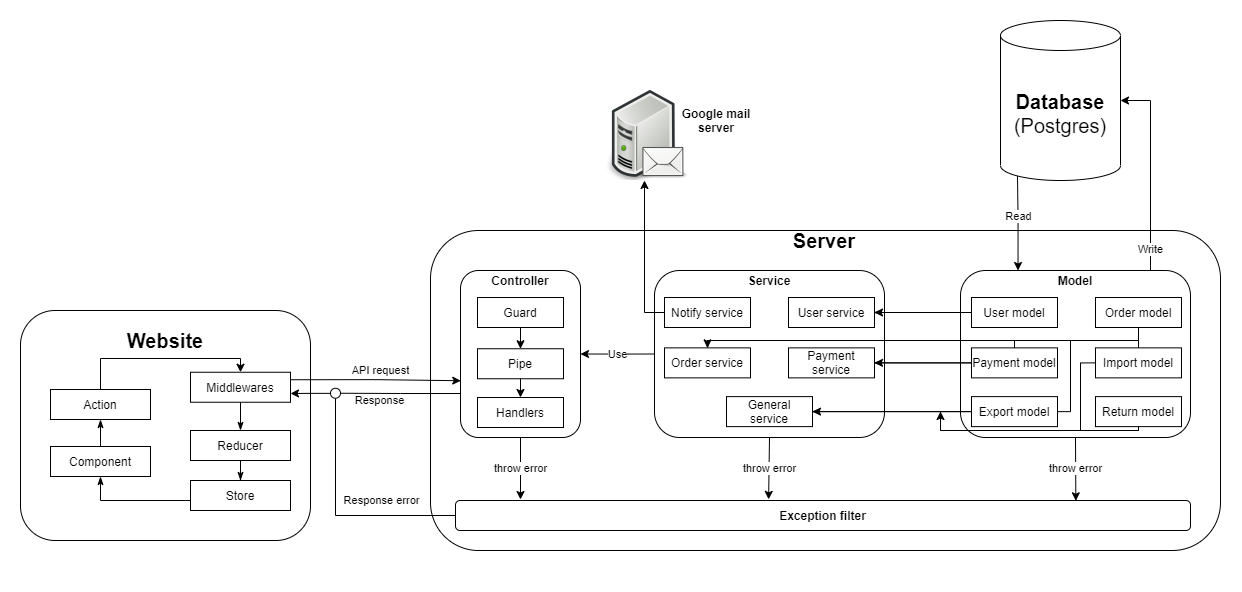
\includegraphics[width=16cm]{Image/Technical/architecture.png}
        \caption{Kiến trúc hệ thống}
        \label{architecture}
    \end{center}
\end{figure}

Kiến trúc của hệ thống được thiết kế như Hình \ref{architecture} bao gồm các thành phần sau:
\subsubsection{Website (front-end)}
\begin{itemize}
    \item Component: chứa các view hiển thị cho người dùng.
    \item Action: nhận các sự kiện mà người dùng thực hiện.
    \item Middlewares và Reducer xử lí các sự kiện của người dùng, các dữ liệu từ server trả về để tính toán trả về state mới.
    \item Store: lưu tất cả state của ứng dụng.
\end{itemize}
\subsubsection{Server (back-end)}
\begin{itemize}
    \item \textbf{Controller}: nhận request trực tiếp từ người dùng, request đi vào controller sẽ đi qua ba bước (có thể có ngoại lệ) cơ bản bao gồm:
    \begin{itemize}
        \item Guard: xác thực người dùng, xem người dùng có phải là người dùng của hệ thống hay không, nếu đúng, nó có thể xét tiếp vai trò của người dùng đó.
        \item Pipe: xác nhận dữ liệu truyền từ người dùng có đúng định dạng, kiểu. Ngoài ra, nó còn thực hiện chuyển đổi dữ liệu trong một số trường hợp.
        \item Handlers: xử lý request của người dùng, điều khiển, gọi các Service tương ứng để xử lý, và phản hồi kết quả cho người dùng. Một handler có thể gọi cùng lúc nhiều service.
    \end{itemize}
    
    \item \textbf{Services}: nhận yêu cầu từ controller để xử lý một tác vụ nào đó và trả về kết quả. Một service cũng có thể gọi và được gọi từ các service khác. Một service có thể là chủ của một hoặc nhiều model. Service sử dụng model để thao tác với cơ sở dữ liệu chứ không trực tiếp làm việc này.
    \begin{itemize}
        \item User service: Service chịu trách nhiệm quản lý user trong hệ thống. Mỗi khi user login vào hệ thống thì sẽ vào Service này để authen: Ban đầu user được yêu cầu sẽ nhập email và password, Sau khi authen là đúng user đó thì hệ thống sẽ sinh ra mã Token để gửi trả về cho user. Sau này cứ mỗi request lên hệ thống thì user sẽ gửi kèm theo mã Token để hệ thống có thể authen và author.
        \item Order Service: Service chịu trách nhiệm tạo, xử lý, lưu trữ các thông tin về đơn đặt hàng cho xưởng nhuộm.
        \item Notify Service: Service chịu trách nhiệm quản lý các thông báo cho hệ thống.
        \item Payment Service: Service chịu trách nhiệm quản lý các thông tin về thanh toán giữa doanh nghiệp và các xưởng nhuộm.
        \item General service: Service chịu trách nhiệm xử lí các nghiệp vụ business chung của hệ thống. Service này gồm nhiều Service tạo thành, có chức năng riêng lẻ.
    \end{itemize}
    
    \item \textbf{Models} là thành phần thao tác trực tiếp với CSDL. Một model ánh xạ chính xác một quan hệ từ cơ sở dữ liệu và các ràng buộc liên quan, các model có tên tương ứng. Các model có mối liên hệ với nhau bằng mối liên hệ của đối tượng.
    
    \item \textbf{Exception Filter} được dành riêng cho việc bắt các lỗi exception và phản hồi lỗi về cho người dùng. Việc chỉ định vai trò này cho một mình Exception Filter thể hiện rõ tính module hoá.

\end{itemize}
Các lớp thành phần ở trên độc lập với nhau, không xung đột lẫn nhau. Mỗi lớp cần thông tin sẽ gọi về lớp thấp hơn, cũng như cung cấp thông tin cho lớp cao hơn.

\subsubsection{Database}
Cơ sở dữ liệu là nơi lưu trữ tất cả dữ liệu cần thiết của ứng dụng, đảm bảo có thế truy cập bất cứ lúc nào và bất cứ đâu. Các quan hệ trong cơ sở dữ liệu được ánh xạ và làm việc trực tiếp với lớp Models. Cơ sở dữ liệu sẽ thực hiện mọi câu lệnh SQL để query dữ liệu, update dữ liệu. tạo mới dữ liệu,...

\newpage
\subsection{Thiết kế cơ sở dữ liệu}
\begin{figure}[H]
    \begin{center}
        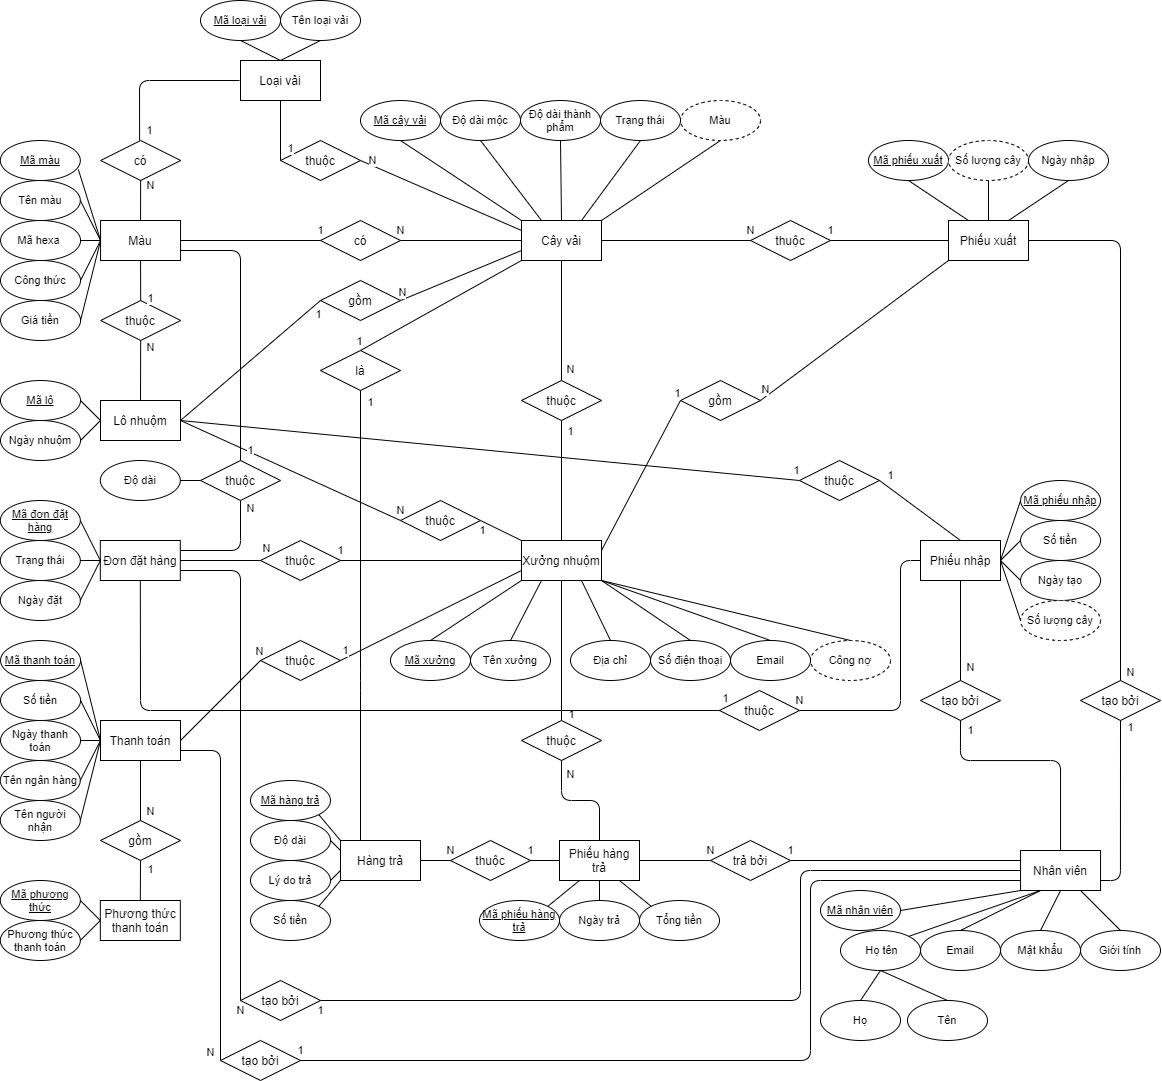
\includegraphics[width=17cm]{Image/General/ERD.png}
        \caption{Mô hình ERD của hệ thống}
        \label{erd}
    \end{center}
\end{figure}
\newpage
Cơ sở dữ liệu của hệ thống được thiết kế dựa trên mô hình  ERD như Hình \ref{erd}

Từ mô hình trên ánh xạ ra mô hình CSDL quan hệ với các bảng được mô tả trong Hình \ref{relation_model}.

\begin{figure}[H]
    \begin{center}
        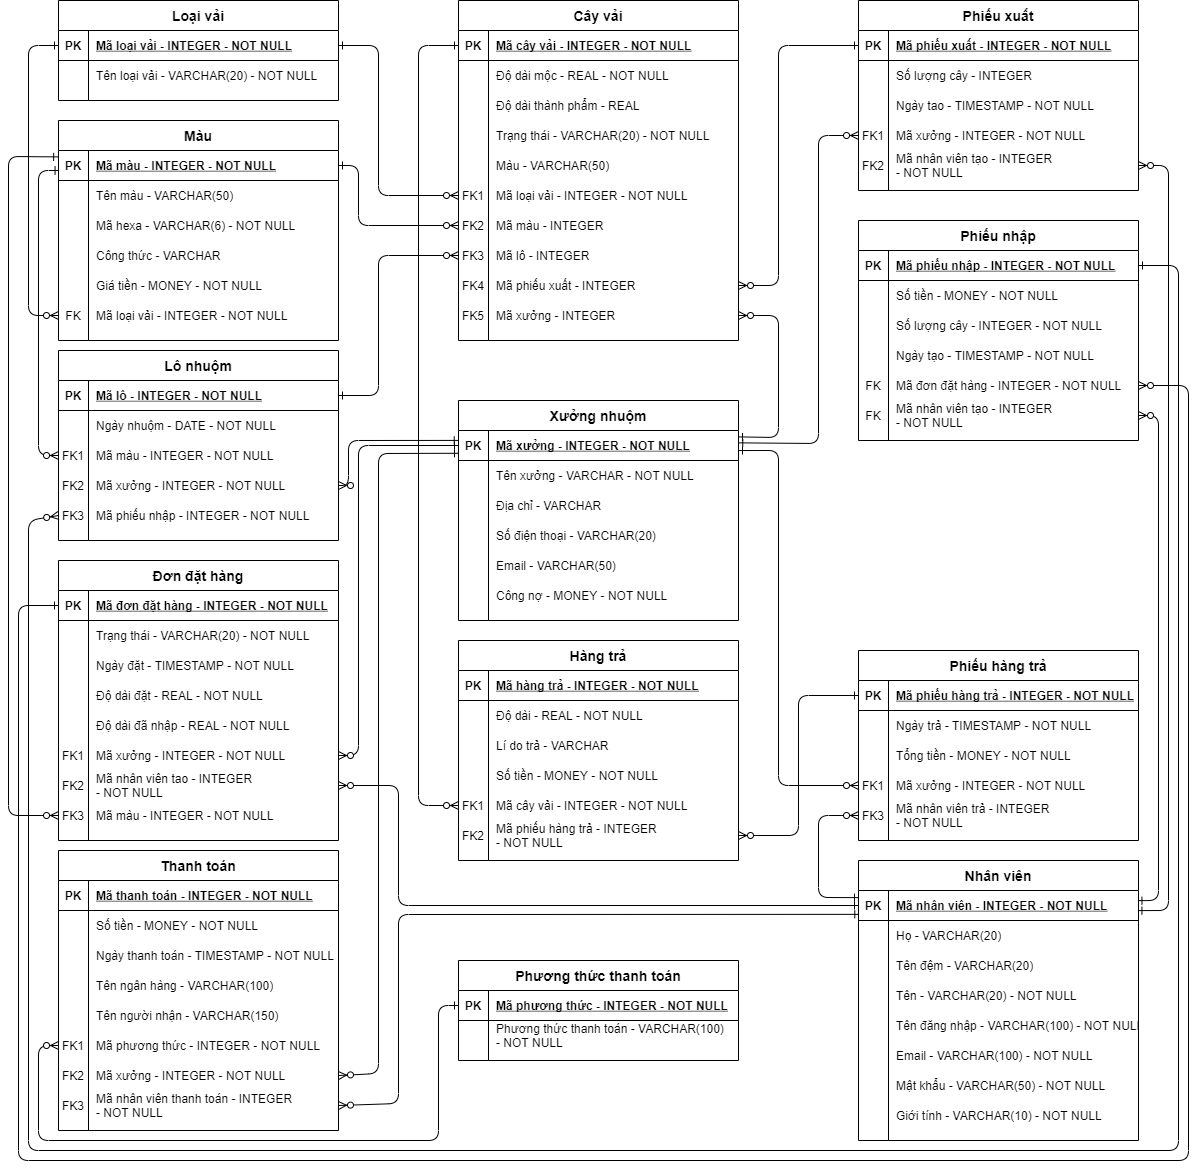
\includegraphics[width=17cm]{Image/General/Relational Data Model.png}
        \caption{Mô hình CSDL quan hệ của hệ thống}
        \label{relation_model}
    \end{center}
\end{figure}

\newpage
Sau khi thiết kế ERD nhóm tiến hành chuyển đổi thành các bảng tương ứng trong database như sau:
\begin{itemize}
    \item \textbf{fabric\_type}
    \begin{table}[H]
        \centering
        \begin{tabular}{|m{3cm}|m{10cm}|}
        \hline 
            id & Mã loại vải\\ \hline
            type & Kí hiệu loại vải \\ \hline
            name & Tên loại vải\\
        \hline 
        \end{tabular}
        \caption{Loại vải}
        \label{fabric_type}
    \end{table}
    
    \item \textbf{color}
    \begin{table}[H]
        \centering
        \begin{tabular}{|m{3cm}|m{10cm}|}
        \hline 
            id & Mã màu\\ \hline
            type & Kí hiệu màu \\ \hline
            name & Tên màu\\ \hline
            hexa\_code & Mã hexa của màu \\ \hline
            recipe & Công thức để thực hiện màu \\ \hline
            price & Giá tiền thi công nhuộm của loại vải và màu tương ứng \\ \hline
            fabric\_type\_id & Mã loại vải \\ 
        \hline 
        \end{tabular}
        \caption{Màu}
        \label{color}
    \end{table}
    
    \item \textbf{dyehouse}
    \begin{table}[H]
        \centering
        \begin{tabular}{|m{3cm}|m{10cm}|}
        \hline 
            id & Mã xưởng nhuộm\\ \hline
            name & Tên xưởng nhuộm \\ \hline
            address & Địa chỉ của xưởng nhuộm\\ \hline
            phone\_number & Số điện thoại của xưởng nhuộm \\ \hline
            email & Email của xưởng nhuộm\\ \hline
            debt & Công nợ hiện tại của xưởng nhuộm\\
        \hline 
        \end{tabular}
        \caption{Xưởng nhuộm}
        \label{dyehouse}
    \end{table}
    
    \item \textbf{users}
    \begin{table}[H]
        \centering
        \begin{tabular}{|m{3cm}|m{10cm}|}
        \hline 
            id & Mã người dùng\\ \hline
            first\_name & Họ người dùng \\ \hline
            last\_name & Tên người dùng\\ \hline
            email & Email của người dùng, tên đăng nhập của tài khoản \\ \hline
            password & Password của tài khoản\\ \hline
            sex & Giới tính của người dùng\\
        \hline 
        \end{tabular}
        \caption{Người dùng}
        \label{users}
    \end{table}
    
    \newpage
    \item \textbf{roles}
    \begin{table}[H]
        \centering
        \begin{tabular}{|m{3cm}|m{10cm}|}
        \hline 
            id & Mã vai trò\\ \hline
            name & Tên vai trò\\
        \hline 
        \end{tabular}
        \caption{Vai trò}
        \label{roles}
    \end{table}
    
    \item \textbf{users\_roles}
    \begin{table}[H]
        \centering
        \begin{tabular}{|m{3cm}|m{10cm}|}
        \hline 
            id & Mã người dùng - vai trò\\ \hline
            users\_id & Mã người dùng\\ \hline
            roles\_id & Mã vai trò\\
        \hline 
        \end{tabular}
        \caption{Người dùng - Vai trò}
        \label{users_roles}
    \end{table}
    
    \item \textbf{persistent\_login}
    \begin{table}[H]
        \centering
        \begin{tabular}{|m{3cm}|m{10cm}|}
        \hline 
            id & Mã persistent login\\ \hline
            user\_id & Mã người dùng\\ \hline
            token & Mã token\\ \hline
            last\_update & Thời gian cập nhận lần cuối\\
        \hline 
        \end{tabular}
        \caption{Persistent login}
        \label{persistent_login}
    \end{table}
    
    \item \textbf{orders}
    \begin{table}[H]
        \centering
        \begin{tabular}{|m{3cm}|m{10cm}|}
        \hline 
            id & Mã đơn đặt hàng\\ \hline
            status & Trạng thái đơn đặt hàng \\ \hline
            create\_date & Ngày tạo đơn đặt hàng \\ \hline
            order\_length & Độ dài đặt\\ \hline
            done\_length & Độ dài thành phẩm\\ \hline
            dyehouse\_id & Mã xưởng nhuộm\\ \hline
            user\_id & Mã người dùng\\ \hline
            color\_id & Mã màu\\
        \hline 
        \end{tabular}
        \caption{Đơn đặt hàng}
        \label{orders}
    \end{table}
    
    \item \textbf{import\_slip}
    \begin{table}[H]
        \centering
        \begin{tabular}{|m{3cm}|m{10cm}|}
        \hline 
            id & Mã phiếu nhập\\ \hline
            money & Số tiền tương ứng với phiếu nhập \\ \hline
            fabric\_number & Số lượng cây vải\\ \hline
            create\_date & Ngày tạo phiếu nhập \\ \hline
            order\_id & Mã đơn đặt hàng\\ \hline
            user\_id & Mã người dùng\\ \hline
            driver & Tên tài xế nhập hàng\\
        \hline 
        \end{tabular}
        \caption{Phiếu nhập}
        \label{import_slip}
    \end{table}
    
    \newpage
    \item \textbf{export\_slip}
    \begin{table}[H]
        \centering
        \begin{tabular}{|m{3cm}|m{10cm}|}
        \hline 
            id & Mã phiếu xuất\\ \hline
            fabric\_number & Số lượng cây vải\\ \hline
            create\_date & Ngày tạo phiếu xuất \\ \hline
            dyehouse\_id & Mã xưởng nhuộm\\ \hline
            user\_id & Mã người dùng\\ 
        \hline 
        \end{tabular}
        \caption{Phiếu xuất}
        \label{export_slip}
    \end{table}
    
    \item \textbf{dye\_batch}
    \begin{table}[H]
        \centering
        \begin{tabular}{|m{3cm}|m{10cm}|}
        \hline 
            id & Mã lô nhuộm\\ \hline
            dye\_date & Ngày nhuộm\\ \hline
            color\_id & Mã màu \\ \hline
            dyehouse\_id & Mã xưởng nhuộm\\ \hline
            import\_slip\_id & Mã phiếu nhập\\ 
        \hline 
        \end{tabular}
        \caption{Lô nhuộm}
        \label{dye_batch}
    \end{table}
    
    \item \textbf{payment\_method}
    \begin{table}[H]
        \centering
        \begin{tabular}{|m{3cm}|m{10cm}|}
        \hline 
            id & Mã phương thức thanh toán\\ \hline
            name & Tên phương thức thanh toán\\ 
        \hline 
        \end{tabular}
        \caption{Phương thức thanh toán}
        \label{payment_method}
    \end{table}
    
    \item \textbf{payment}
    \begin{table}[H]
        \centering
        \begin{tabular}{|m{3.5cm}|m{10cm}|}
        \hline 
            id & Mã thanh toán\\ \hline
            money & Số tiền thanh toán\\ \hline
            create\_date & Ngày thanh toán \\ \hline
            bank\_name & Tên ngân hàng\\ \hline
            recipient\_name & Người nhận thanh toán\\ \hline
            payment\_method\_id & Phương thức thanh toán \\ \hline
            dyehouse\_id & Mã xưởng nhuộm\\ \hline
            user\_id & Mã người dùng\\ 
        \hline 
        \end{tabular}
        \caption{Thanh toán}
        \label{payment}
    \end{table}
    
    \newpage
    \item \textbf{fabric}
    \begin{table}[H]
        \centering
        \begin{tabular}{|m{3cm}|m{10cm}|}
        \hline 
            id & Mã cây vải\\ \hline
            raw\_length & Độ dài thô\\ \hline
            finished\_length & Độ dài thành phẩm \\ \hline
            status & Trạng thái của cây vải\\ \hline
            color\_name & Tên màu\\ \hline
            fabric\_type\_id & Mã loại vải\\ \hline
            color\_id & Mã màu \\ \hline
            dye\_batch\_id & Mã lô nhuộm\\ \hline
            export\_slip\_id & Mã phiếu xuất\\ \hline
            dyehouse\_id & Mã xưởng nhuộm\\ 
        \hline 
        \end{tabular}
        \caption{Cây vải}
        \label{fabric}
    \end{table}

    \item \textbf{return\_slip}
    \begin{table}[H]
        \centering
        \begin{tabular}{|m{3cm}|m{10cm}|}
        \hline 
            id & Mã phiếu hàng trả\\ \hline
            return\_date & Ngày tạo phiếu hàng trả\\ \hline
            money & Số tiền tương ứng với phiếu hàng trả \\ \hline
            received\_name & Tên người nhận hàng trả\\ \hline
            dyehouse\_id & Mã xưởng nhuộm\\ \hline
            user\_id & Mã người dùng\\ 
        \hline 
        \end{tabular}
        \caption{Phiếu hàng trả}
        \label{return_slip}
    \end{table}
    
    \item \textbf{returns}
    \begin{table}[H]
        \centering
        \begin{tabular}{|m{3cm}|m{10cm}|}
        \hline 
            id & Mã hàng trả\\ \hline
            return\_length & Độ dài trả\\ \hline
            return\_reason & Lí do trả \\ \hline
            money & Số tiền tương ứng với hàng trả\\ \hline
            fabric\_id & Mã cây vải\\ \hline
            return\_slip\_id & Mã phiếu hàng trả\\ 
        \hline 
        \end{tabular}
        \caption{Hàng trả}
        \label{returns}
    \end{table}


\end{itemize}


\newpage



\subsection{Thiết kế giao diện}
% Trong phần này, nhóm trình bày các thiết kế giao diện tổng quan của hệ thống. Trong quá trình phát triển, để phù hợp với nghiệp vụ của đề tài, sẽ có một số thay đổi giao diện trong sản phẩm cuối cùng.

%%%%%%%%%%%%%%%%%%%%%%%%%%%%%%%%%%%%%%%
\subsubsection{Trang đăng nhập}

\begin{figure}[H]
    \begin{center}
        \frame{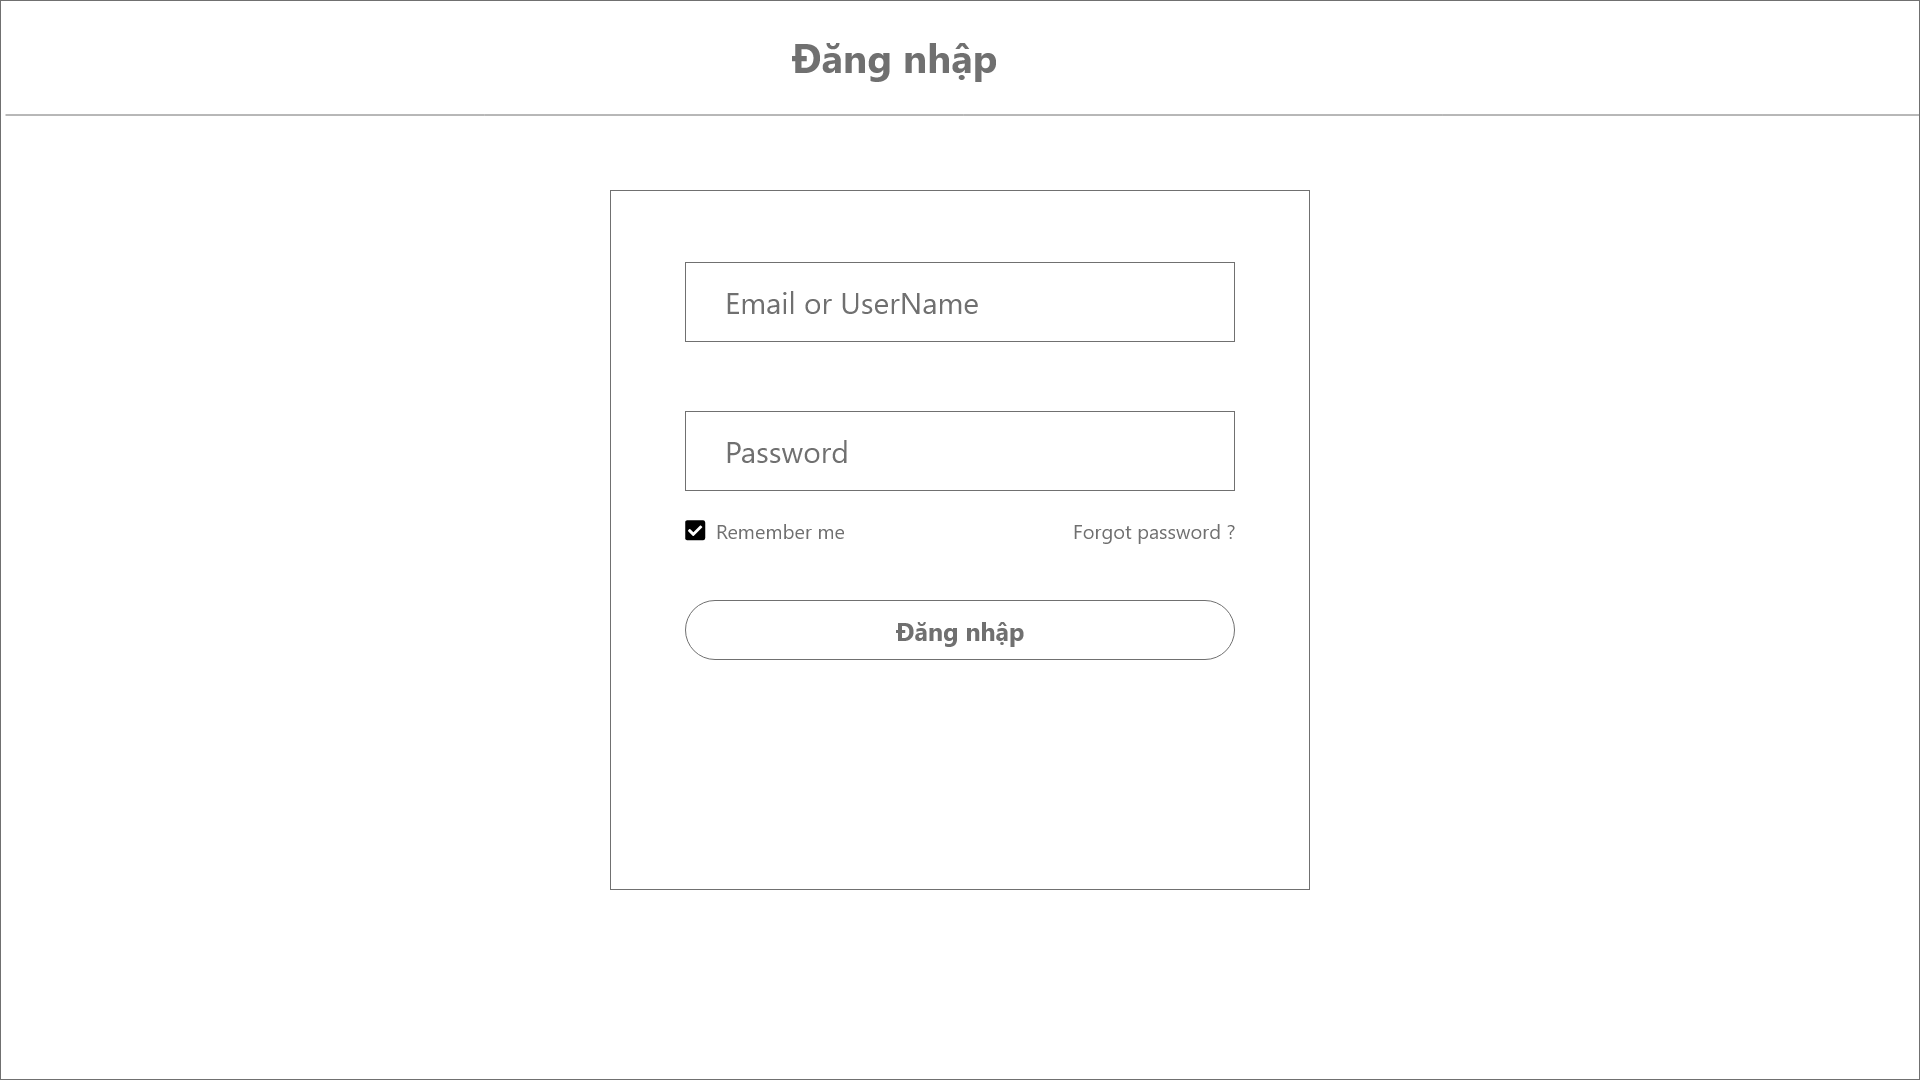
\includegraphics[width=12cm]{Image/Mockup/Sign in.png}}
        \caption{Trang đăng nhập}
        \label{mockup_signin}
    \end{center}
\end{figure}

%%%%%%%%%%%%%%%%%%%%%%%%%%%%%%%%%%%%%%%
\subsubsection{Quản lí xưởng nhuộm}

\begin{figure}[H]
    \begin{center}
        \frame{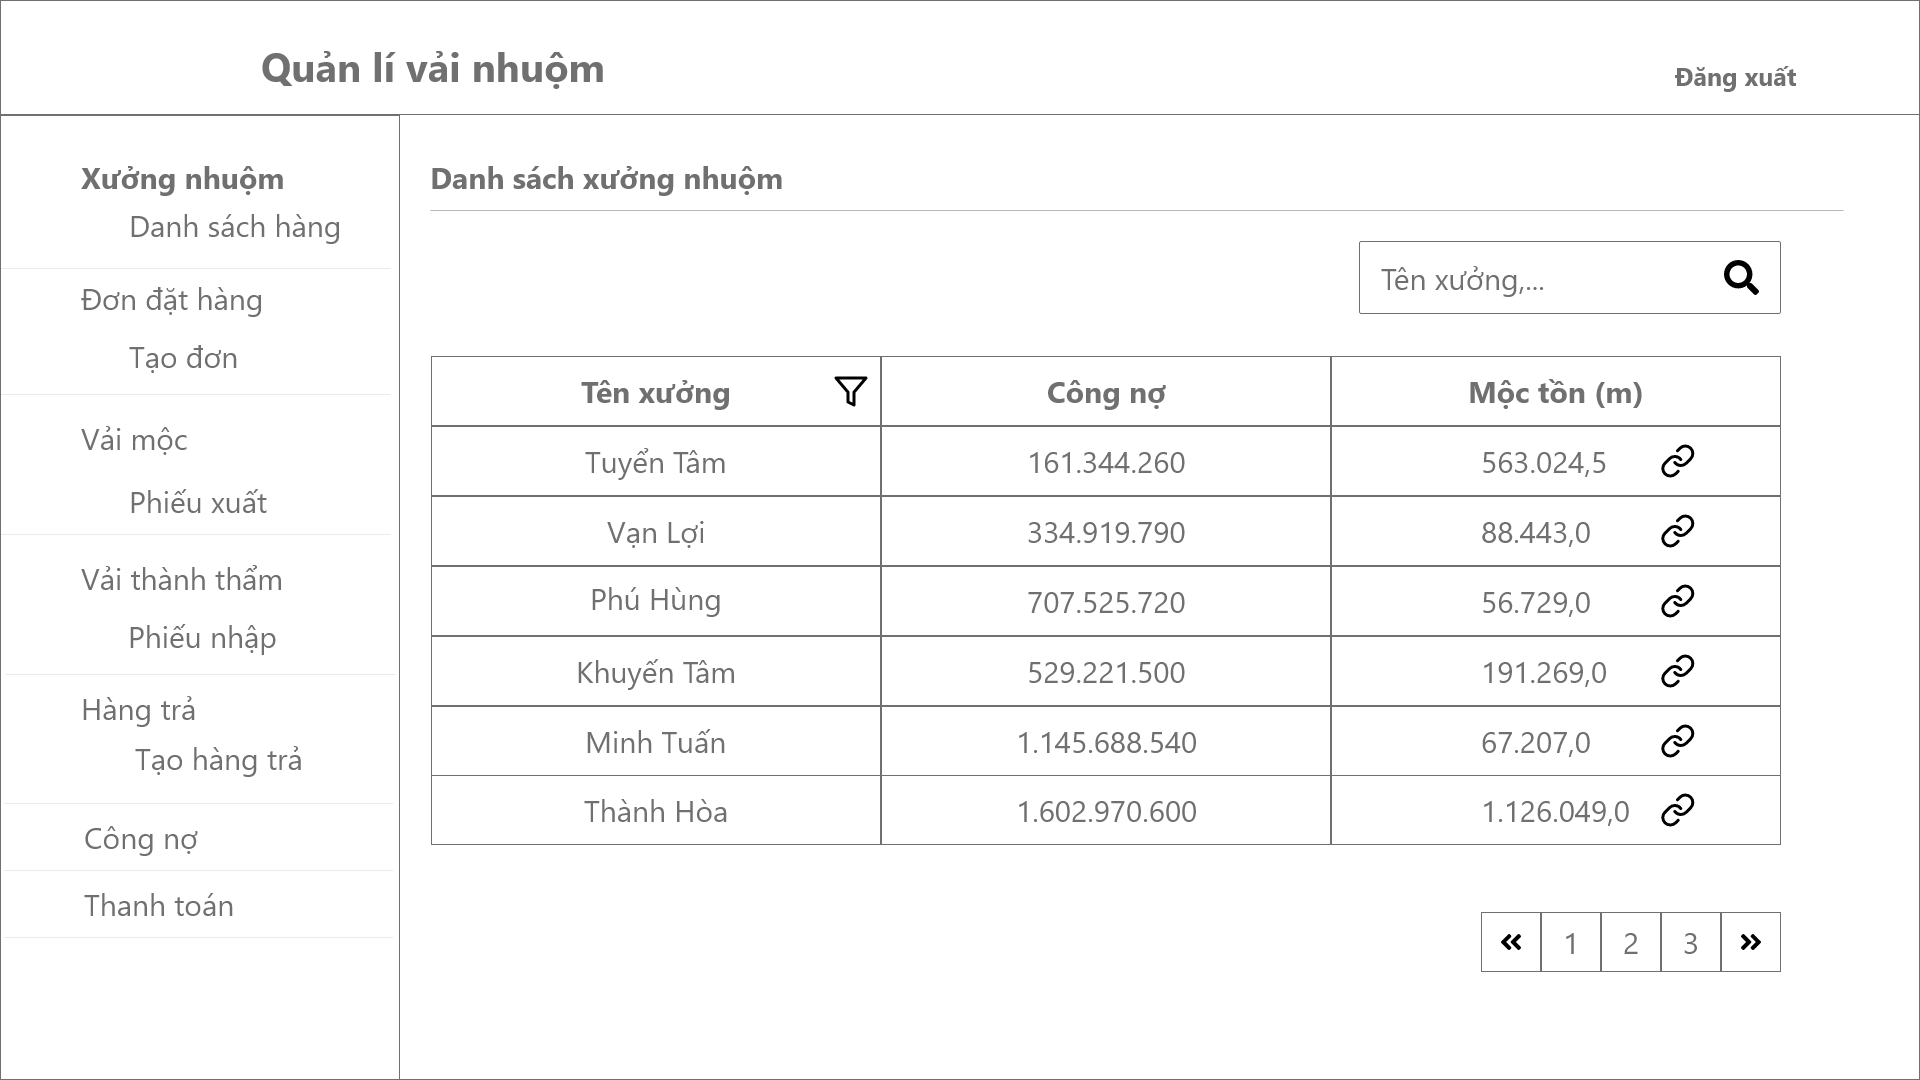
\includegraphics[width=12cm]{Image/Mockup/Danh sách xưởng.png}}
        \caption{Danh sách xưởng nhuộm}
        \label{mockup_homepage}
    \end{center}
\end{figure}

\begin{figure}[H]
    \begin{center}
        \frame{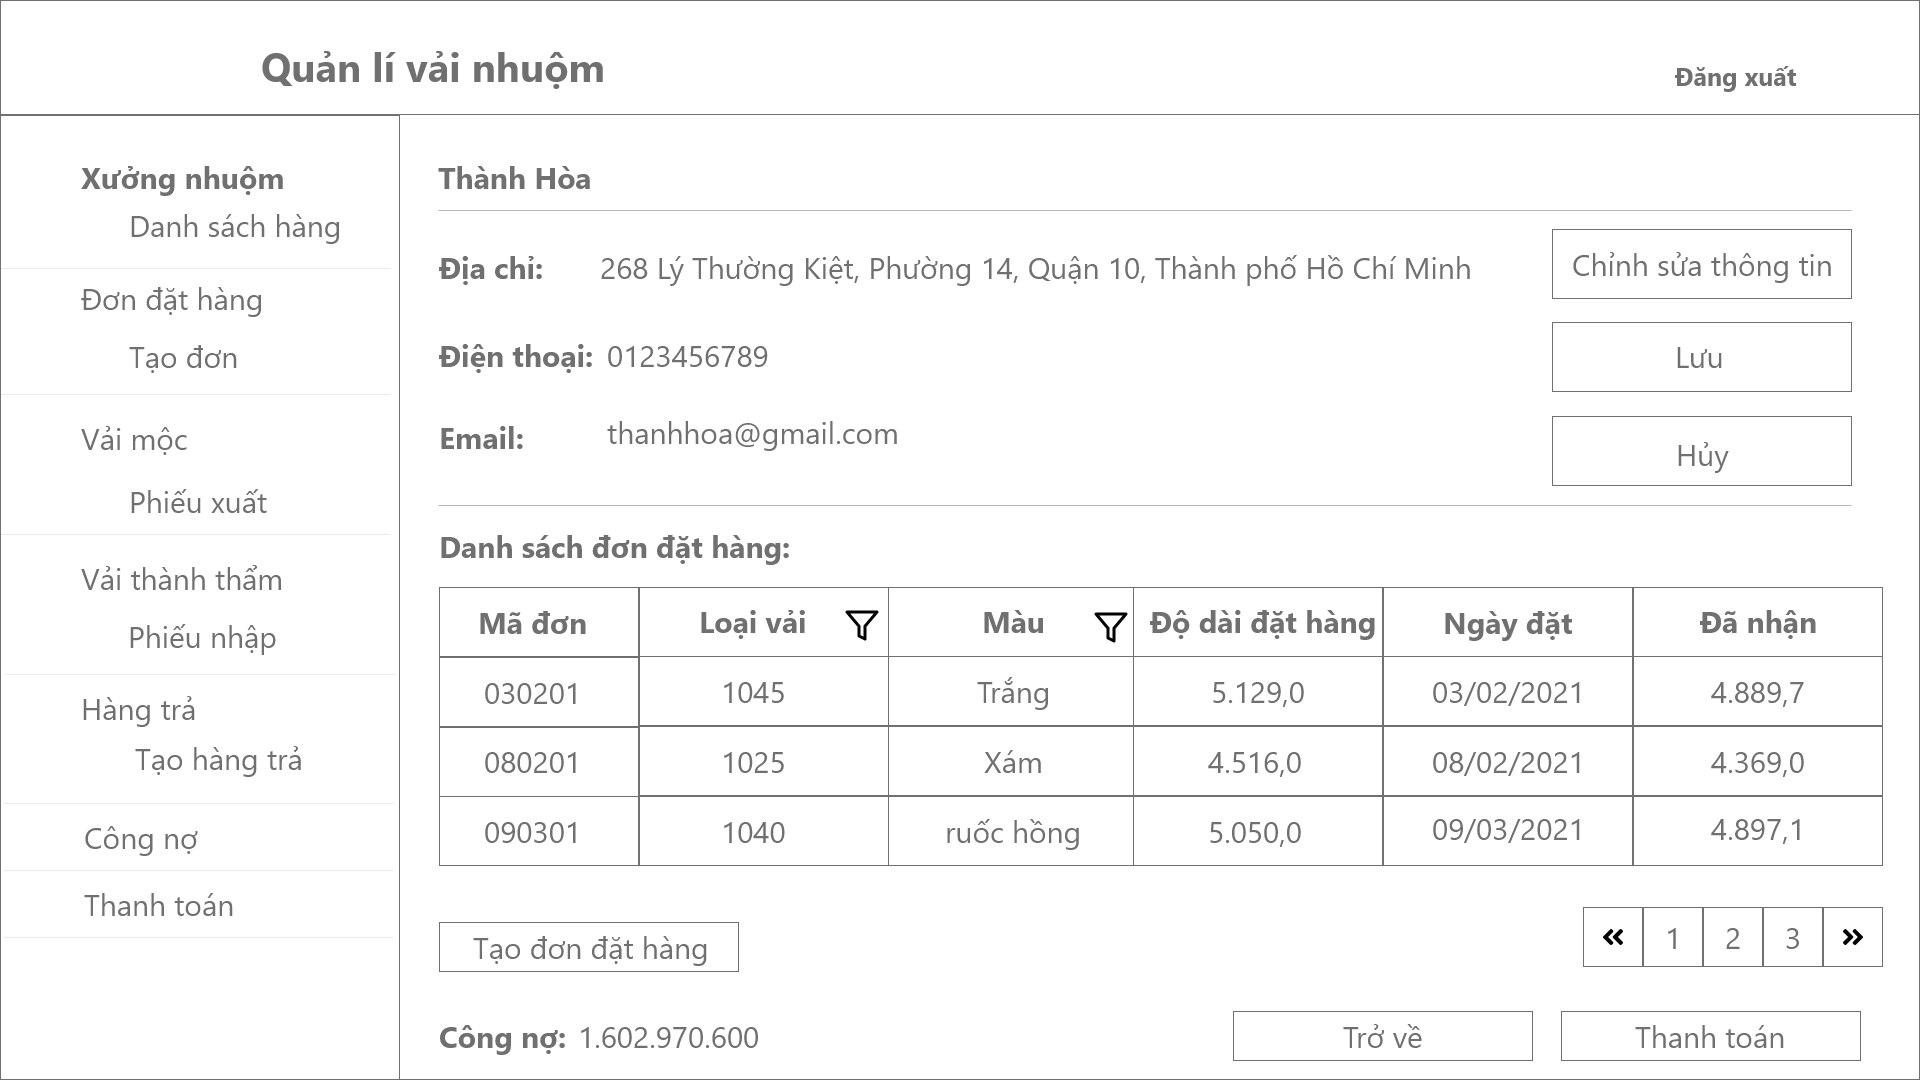
\includegraphics[width=12cm]{Image/Mockup/Chi tiết xưởng.png}}
        \caption{Chi tiết xưởng nhuộm}
        \label{mockup_detail_plant}
    \end{center}
\end{figure}

\begin{figure}[H]
    \begin{center}
        \frame{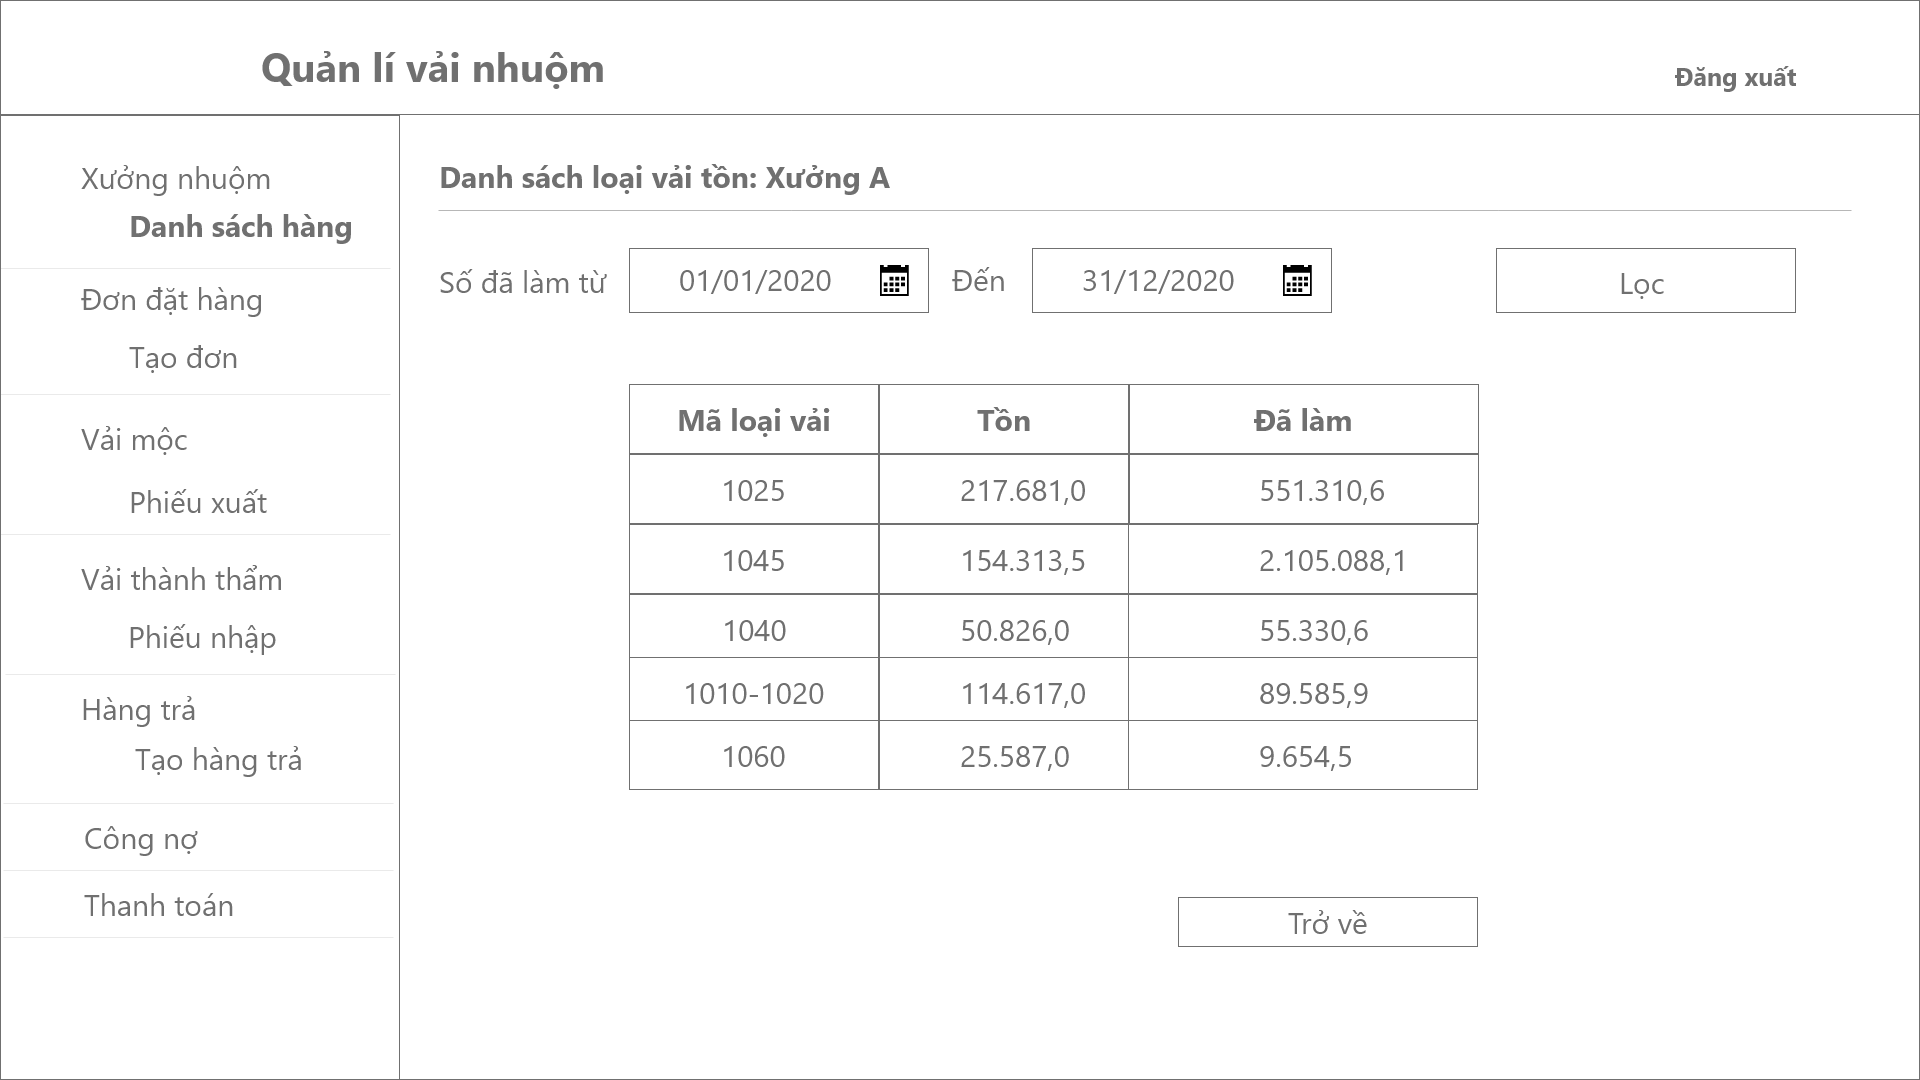
\includegraphics[width=12cm]{Image/Mockup/Chi tiết xưởng - vải tồn.png}}
        \caption{Chi tiết xưởng  - hàng tồn kho}
        \label{mockup_detail_plant-1}
    \end{center}
\end{figure}

%%%%%%%%%%%%%%%%%%%%%%%%%%%%%%%%%%%%%%%
\subsubsection{Quản lí đơn đặt hàng}

\begin{figure}[H]
    \begin{center}
        \frame{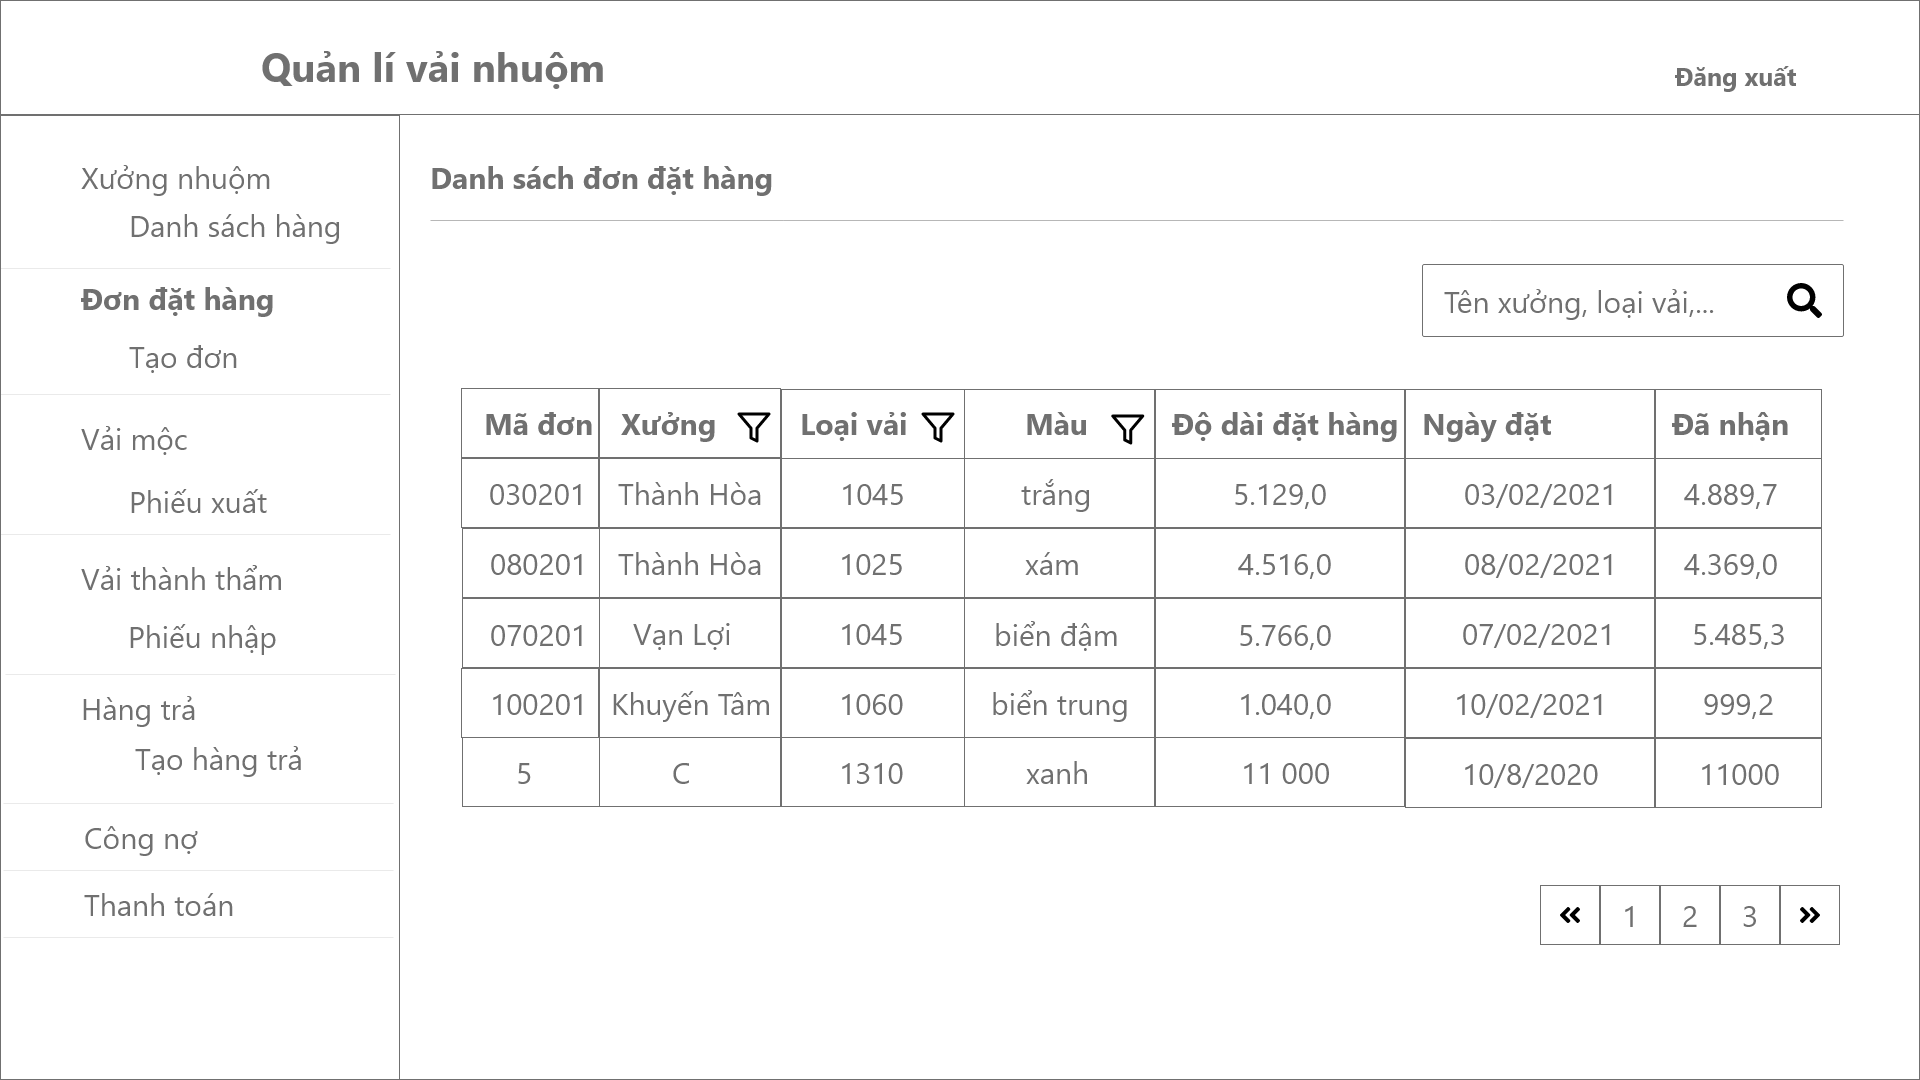
\includegraphics[width=12cm]{Image/Mockup/Danh sách đơn hàng.png}}
        \caption{Danh sách đơn đặt hàng}
        \label{mockup_list_order}
    \end{center}
\end{figure}

\begin{figure}[H]
    \begin{center}
        \frame{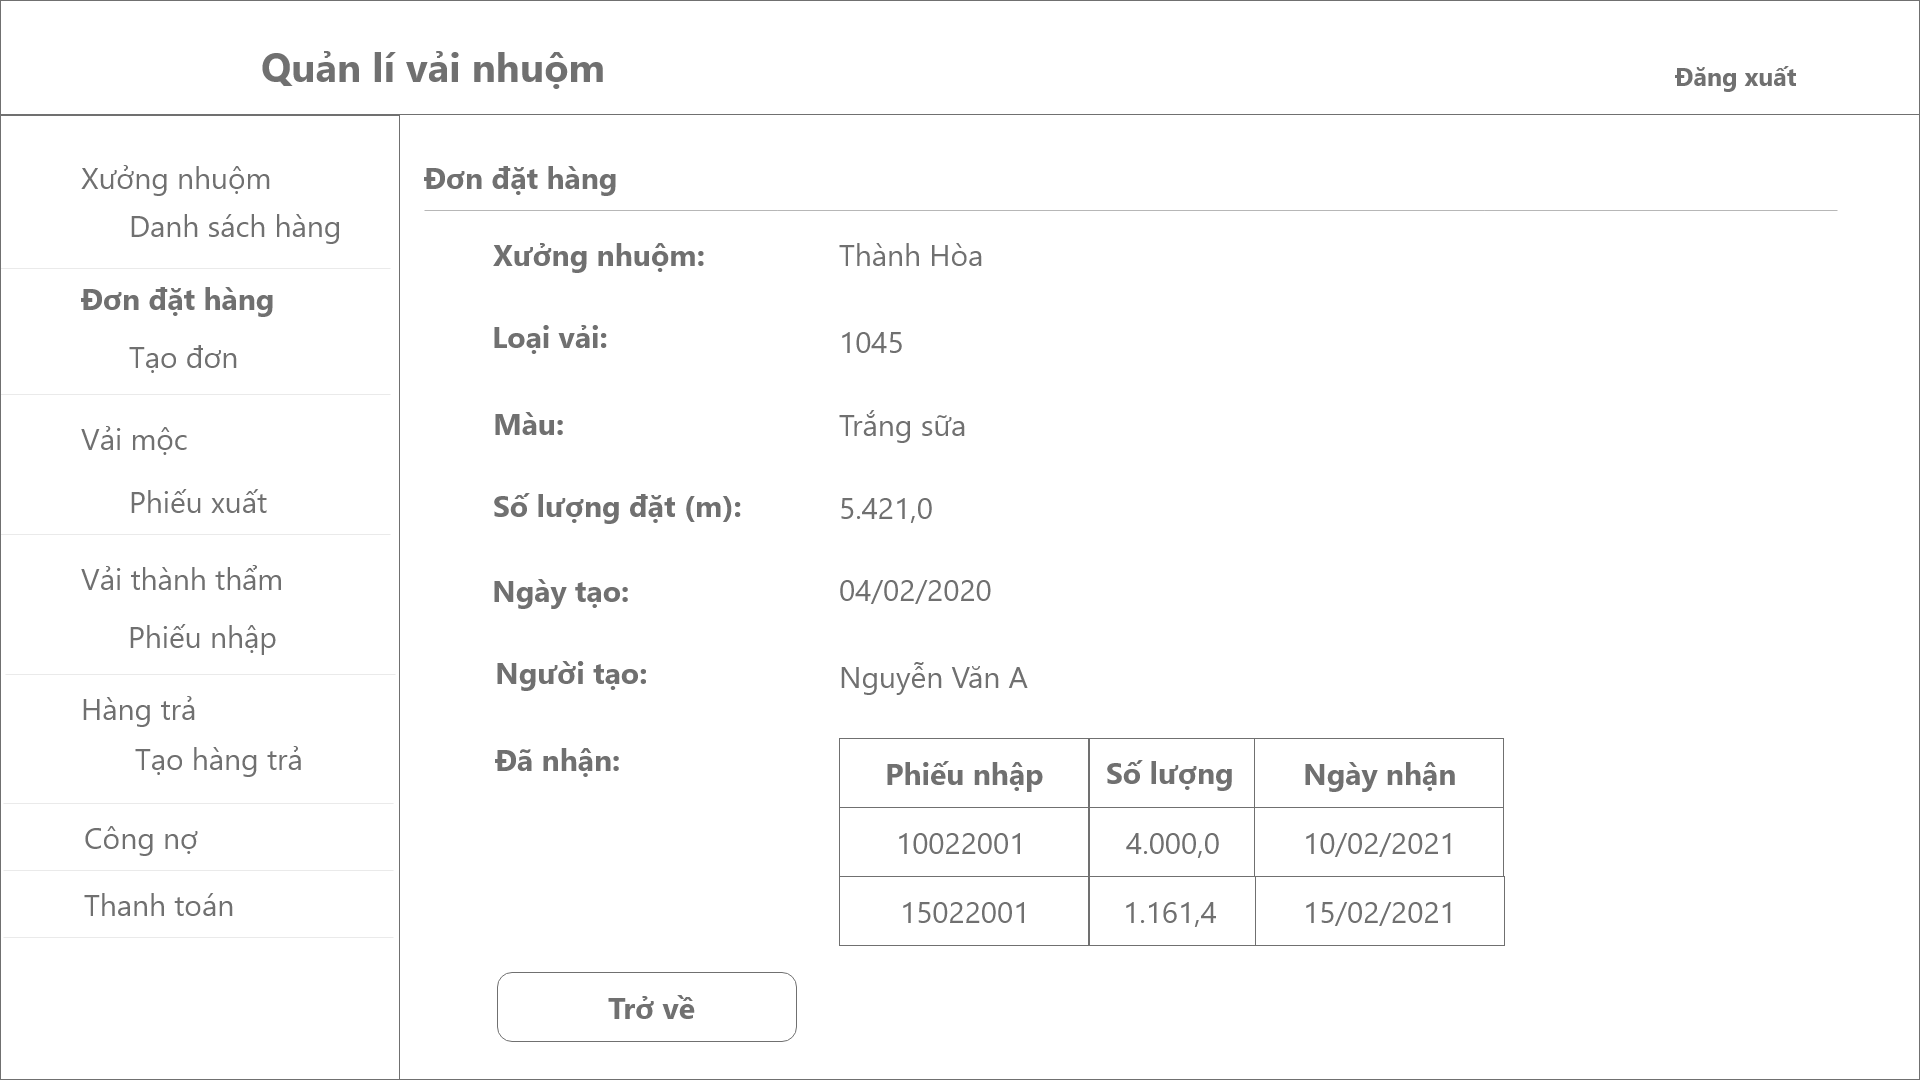
\includegraphics[width=12cm]{Image/Mockup/Chi tiết đơn hàng.png}}
        \caption{Chi tiết đơn đặt hàng}
        \label{mockup_detail_order}
    \end{center}
\end{figure}

\begin{figure}[H]
    \begin{center}
        \frame{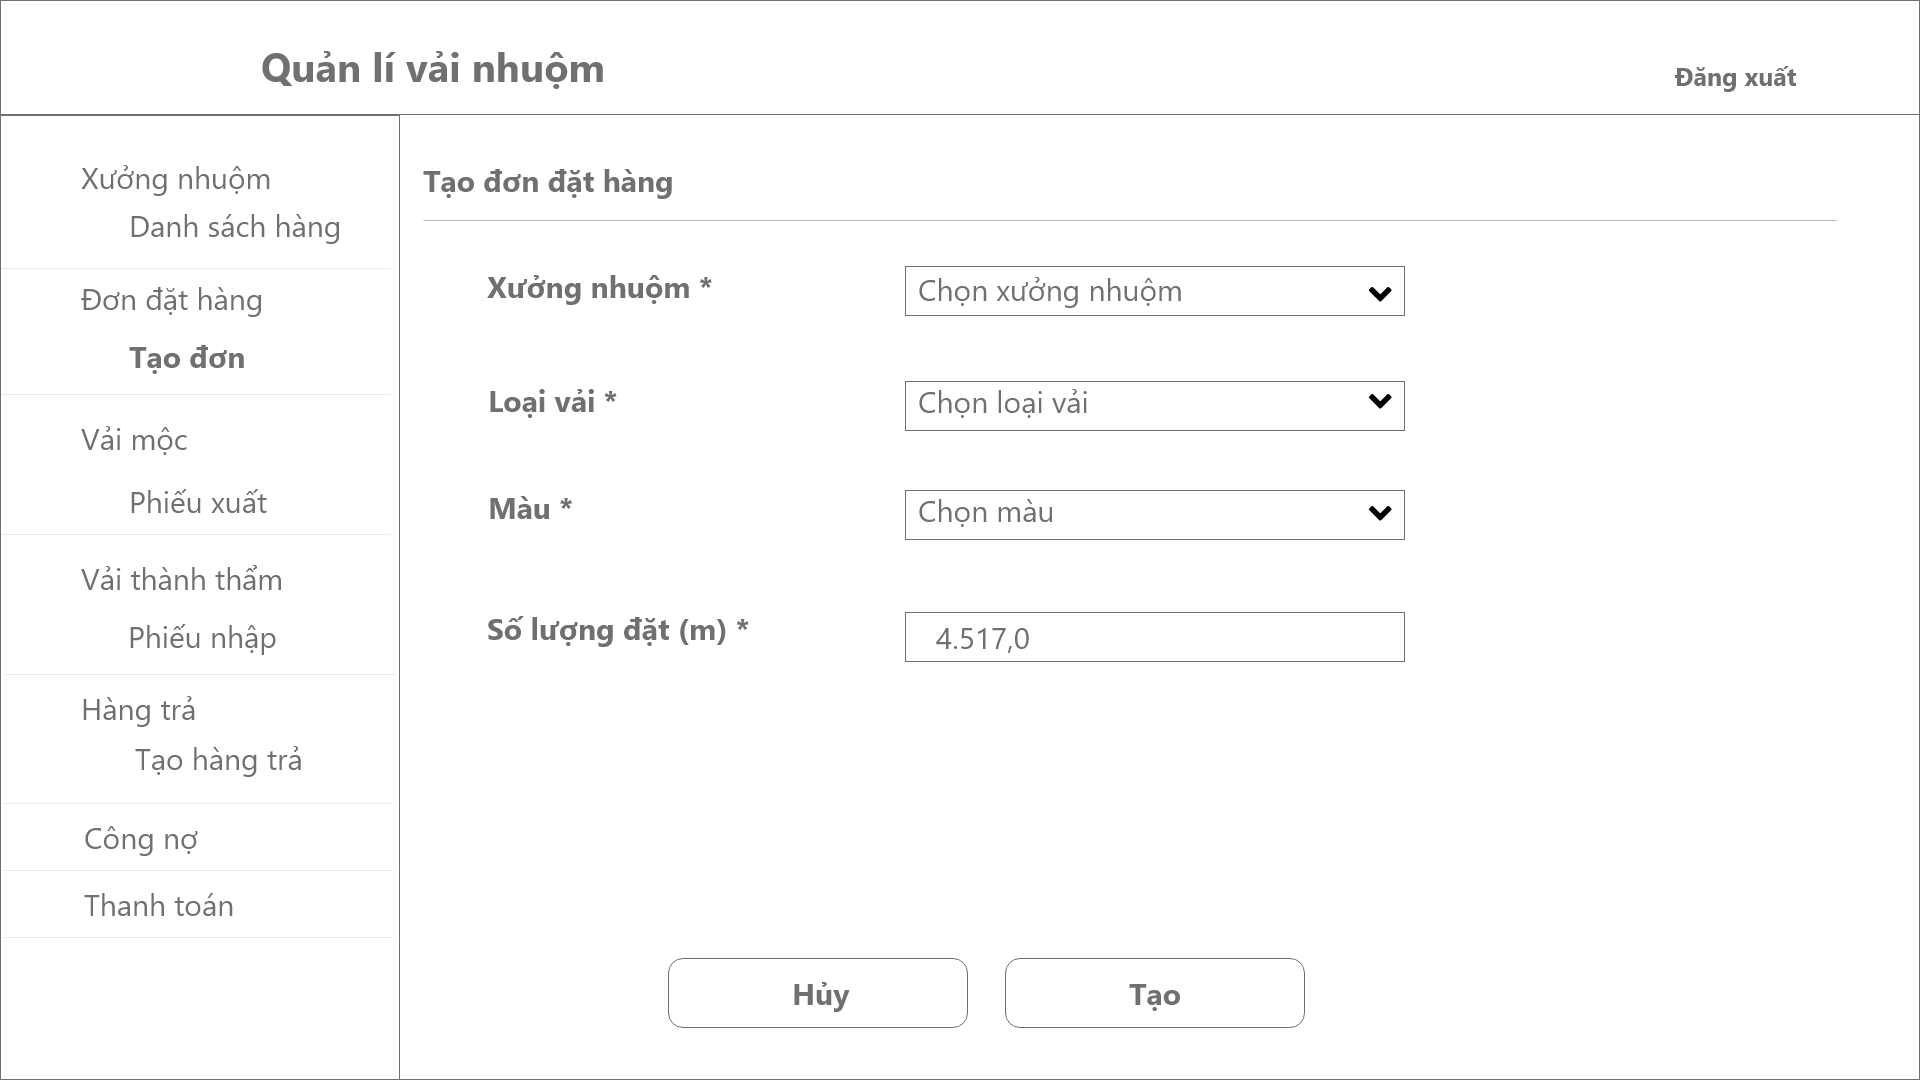
\includegraphics[width=12cm]{Image/Mockup/Tạo đơn hàng.png}}
        \caption{Tạo đơn đặt hàng}
        \label{mockup_create_order}
    \end{center}
\end{figure}

%%%%%%%%%%%%%%%%%%%%%%%%%%%%%%%%%%%%%%%
\subsubsection{Quản lí mộc}

\begin{figure}[H]
    \begin{center}
        \frame{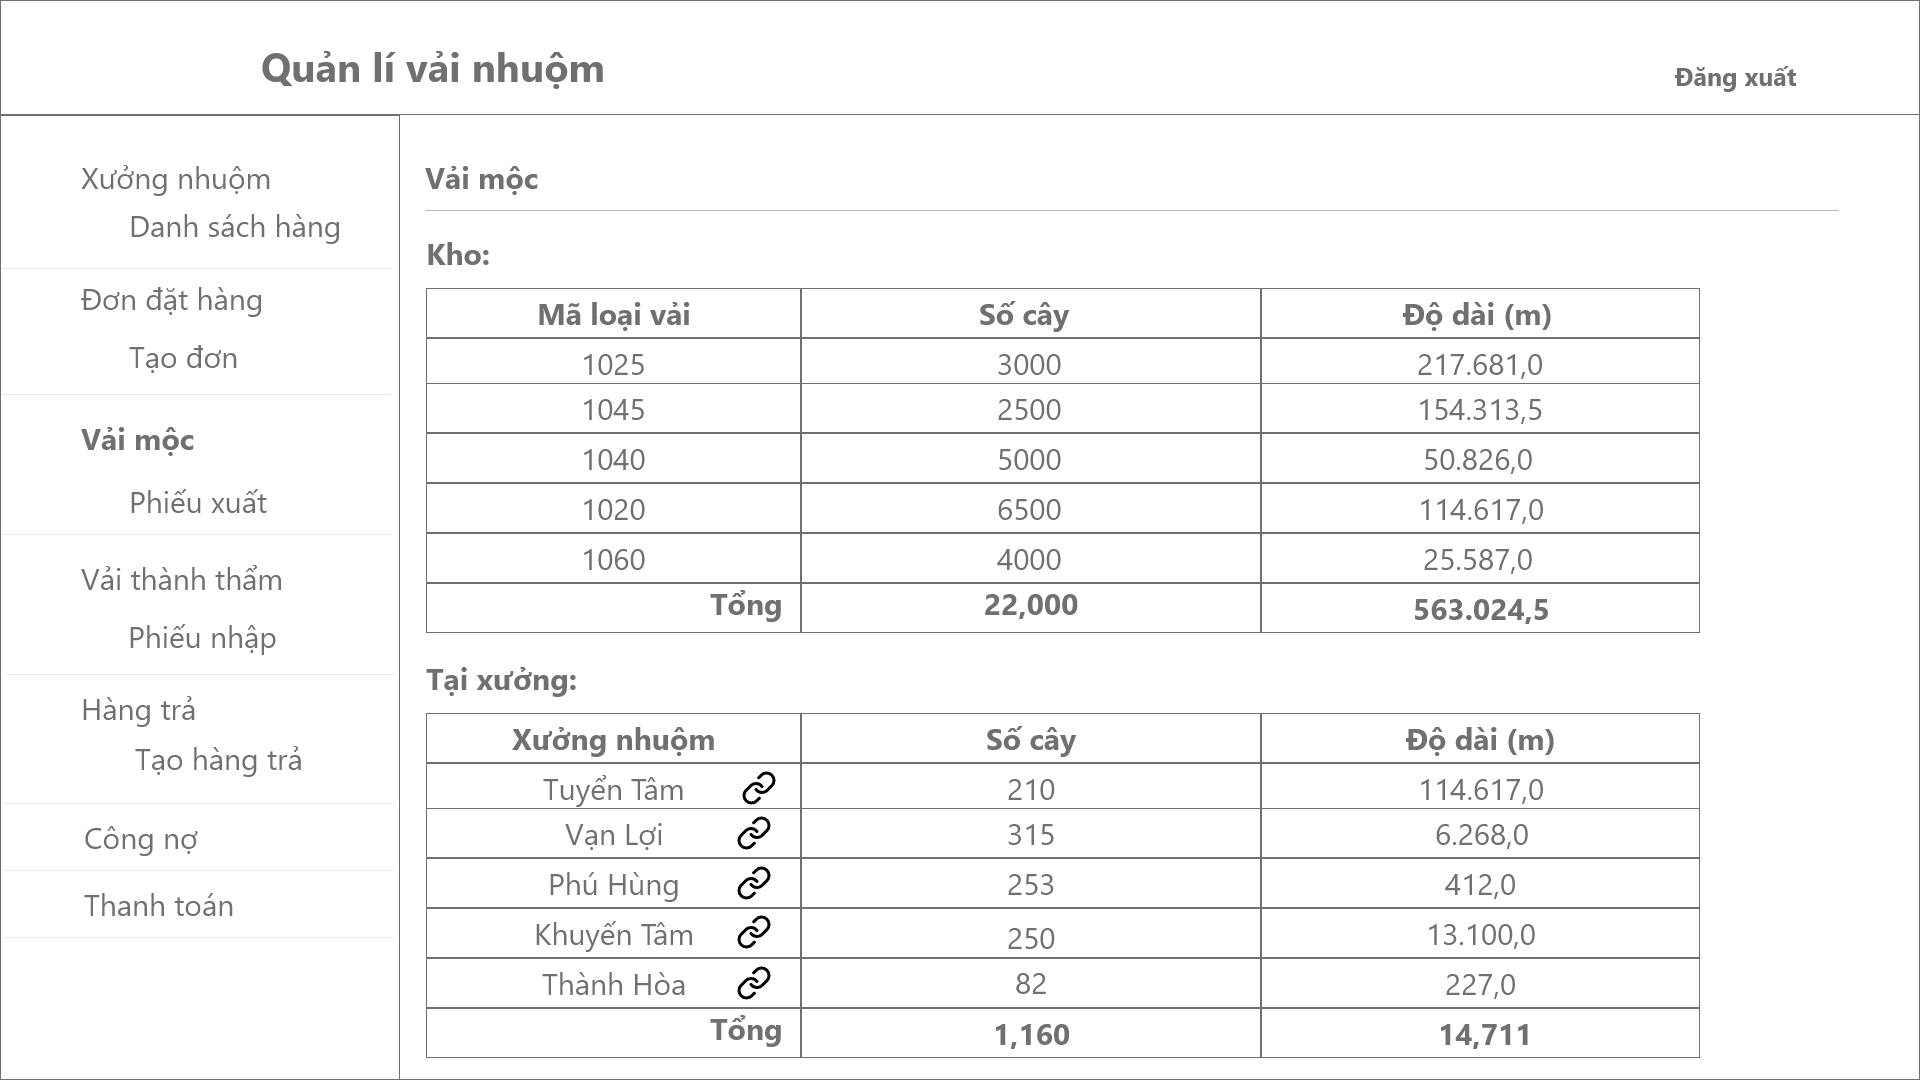
\includegraphics[width=12cm]{Image/Mockup/Vải mộc.png}}
        \caption{Danh sách các loại vải mộc ở kho và tồn ở các xưởng}
        \label{mockup_raw}
    \end{center}
\end{figure}

\begin{figure}[H]
    \begin{center}
        \frame{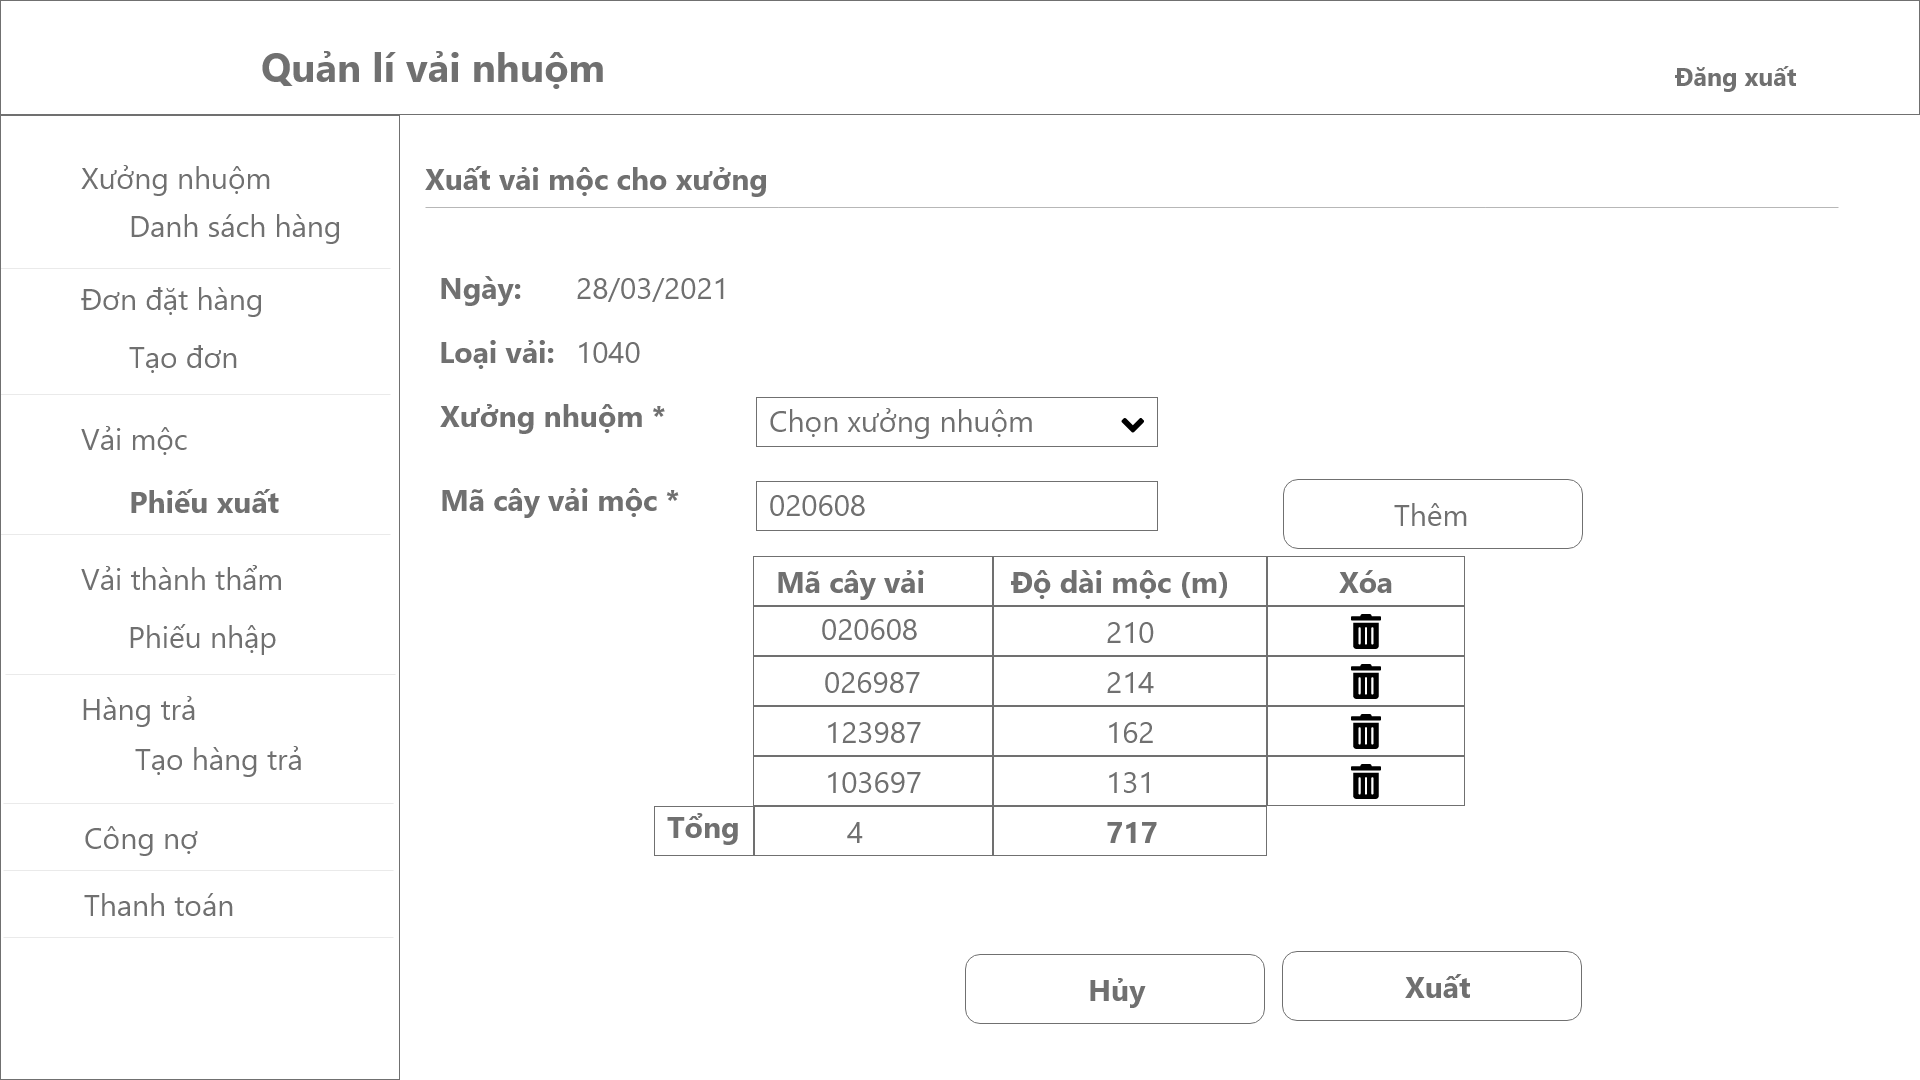
\includegraphics[width=12cm]{Image/Mockup/Xuất vải mộc.png}}
        \caption{Tạo phiếu xuất mộc}
        \label{mockup_export_raw_1}
    \end{center}
\end{figure}

%%%%%%%%%%%%%%%%%%%%%%%%%%%%%%%%%%%%%%%
\subsubsection{Quản lí thành phẩm}

\begin{figure}[H]
    \begin{center}
        \frame{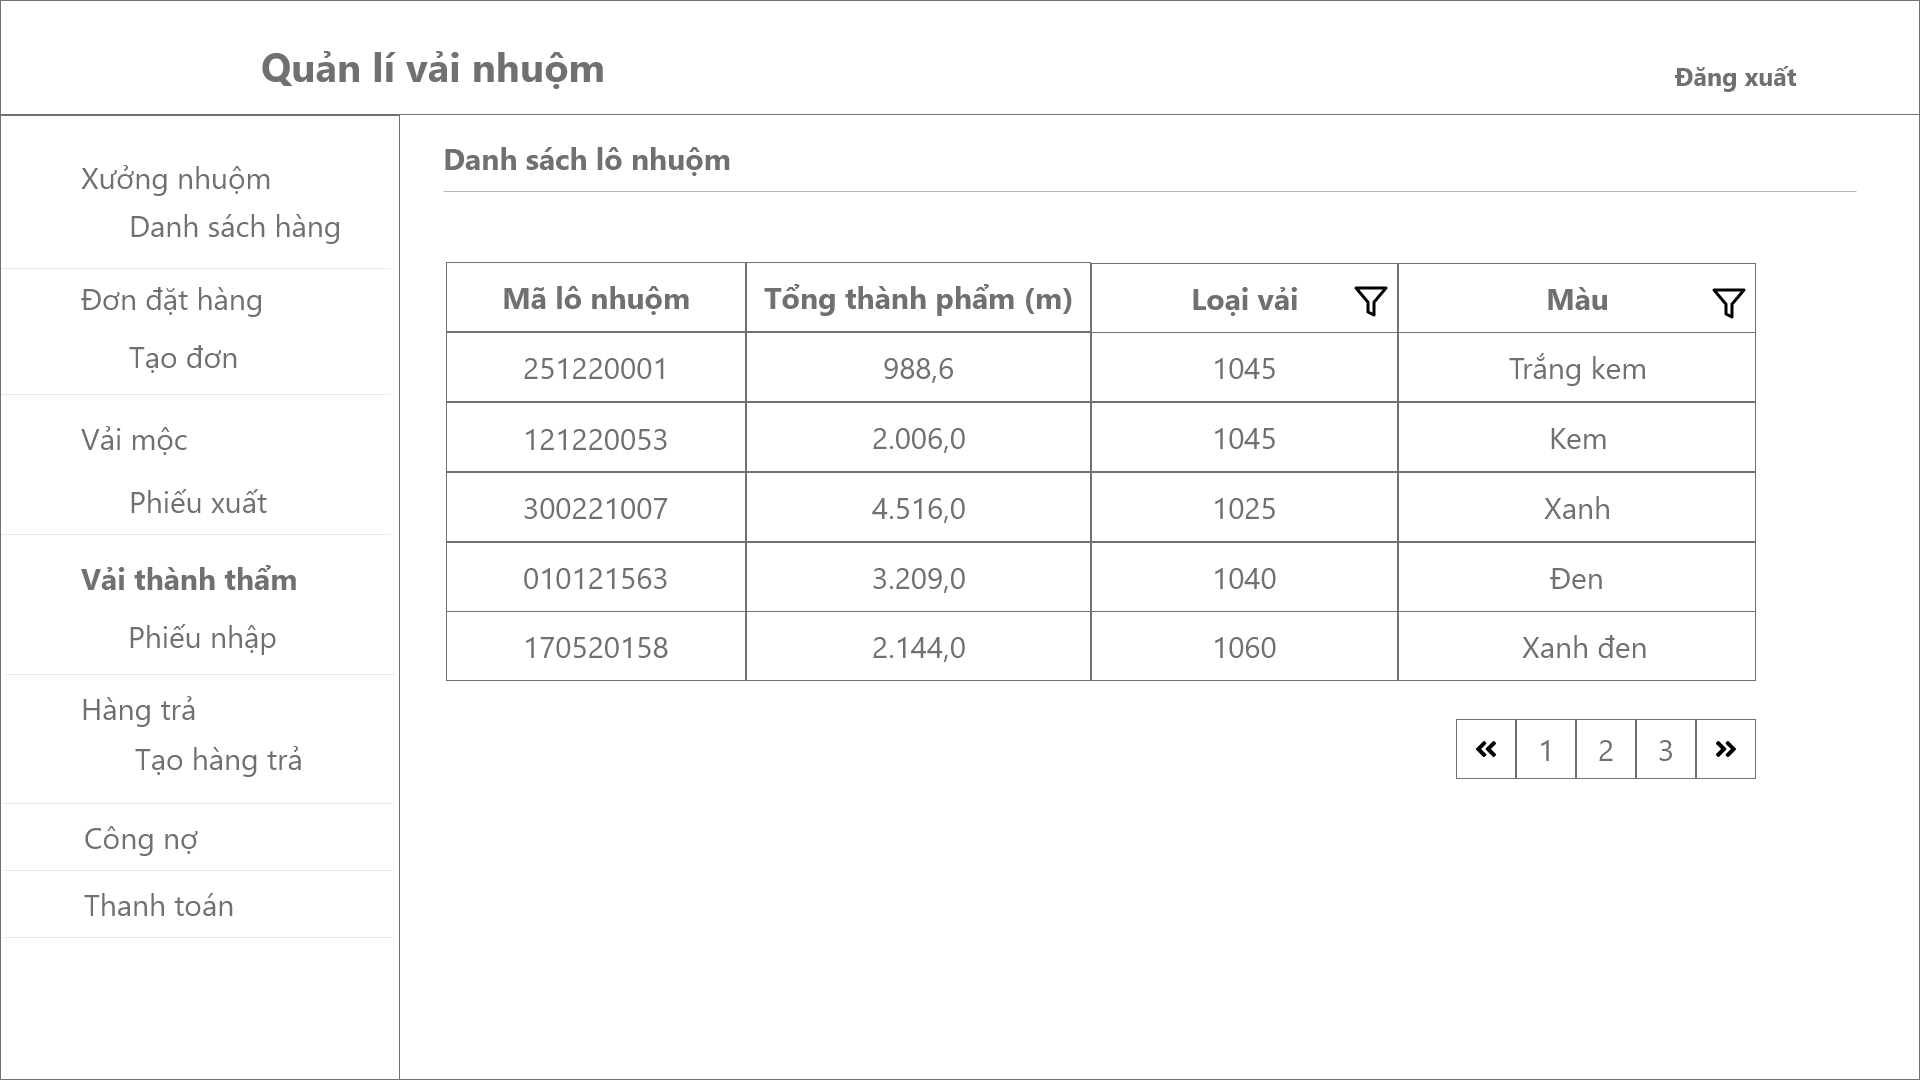
\includegraphics[width=12cm]{Image/Mockup/Danh sách lô nhuộm.png}}
        \caption{Danh sách các phiếu nhập}
        \label{mockup_list_batch}
    \end{center}
\end{figure}

\begin{figure}[H]
    \begin{center}
        \frame{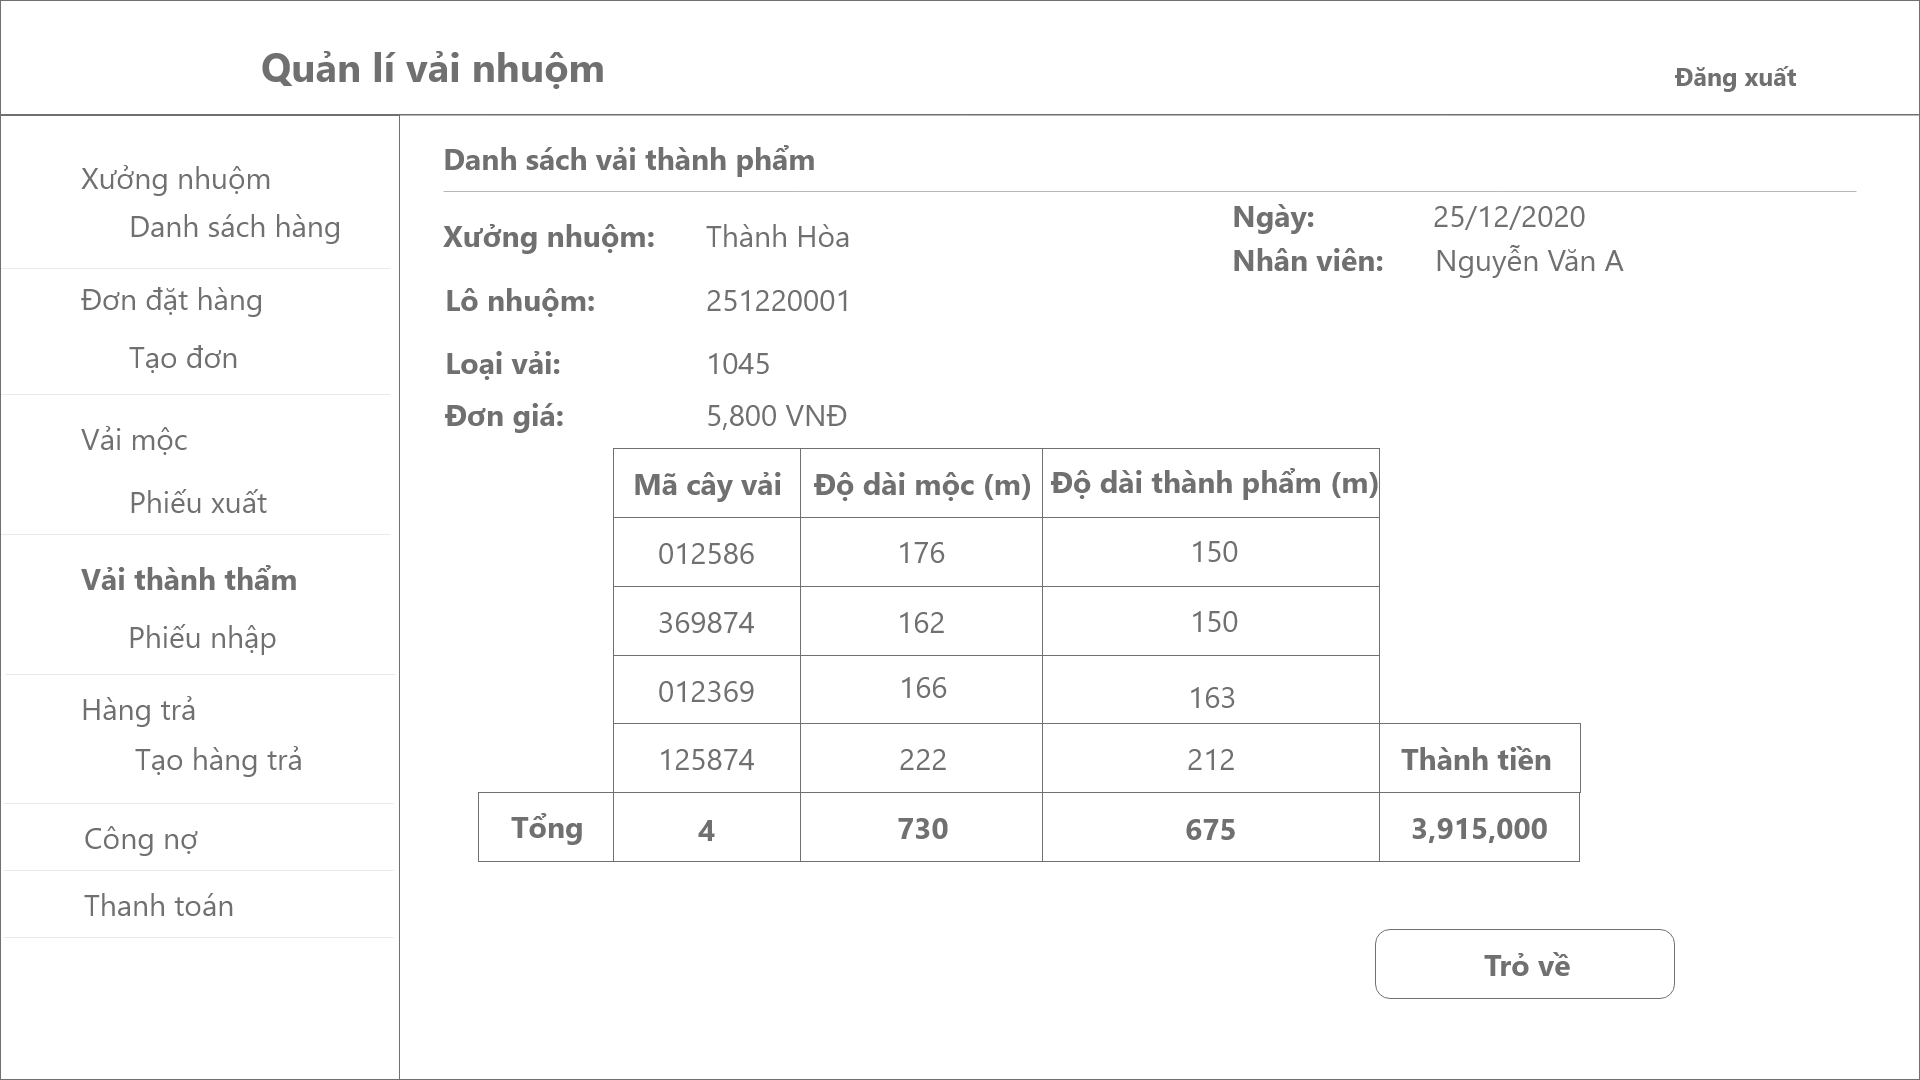
\includegraphics[width=12cm]{Image/Mockup/Chi tiết lô nhuộm.png}}
        \caption{Chi tiết phiếu nhập}
        \label{mockup_detail_batch}
    \end{center}
\end{figure}

\begin{figure}[H]
    \begin{center}
        \frame{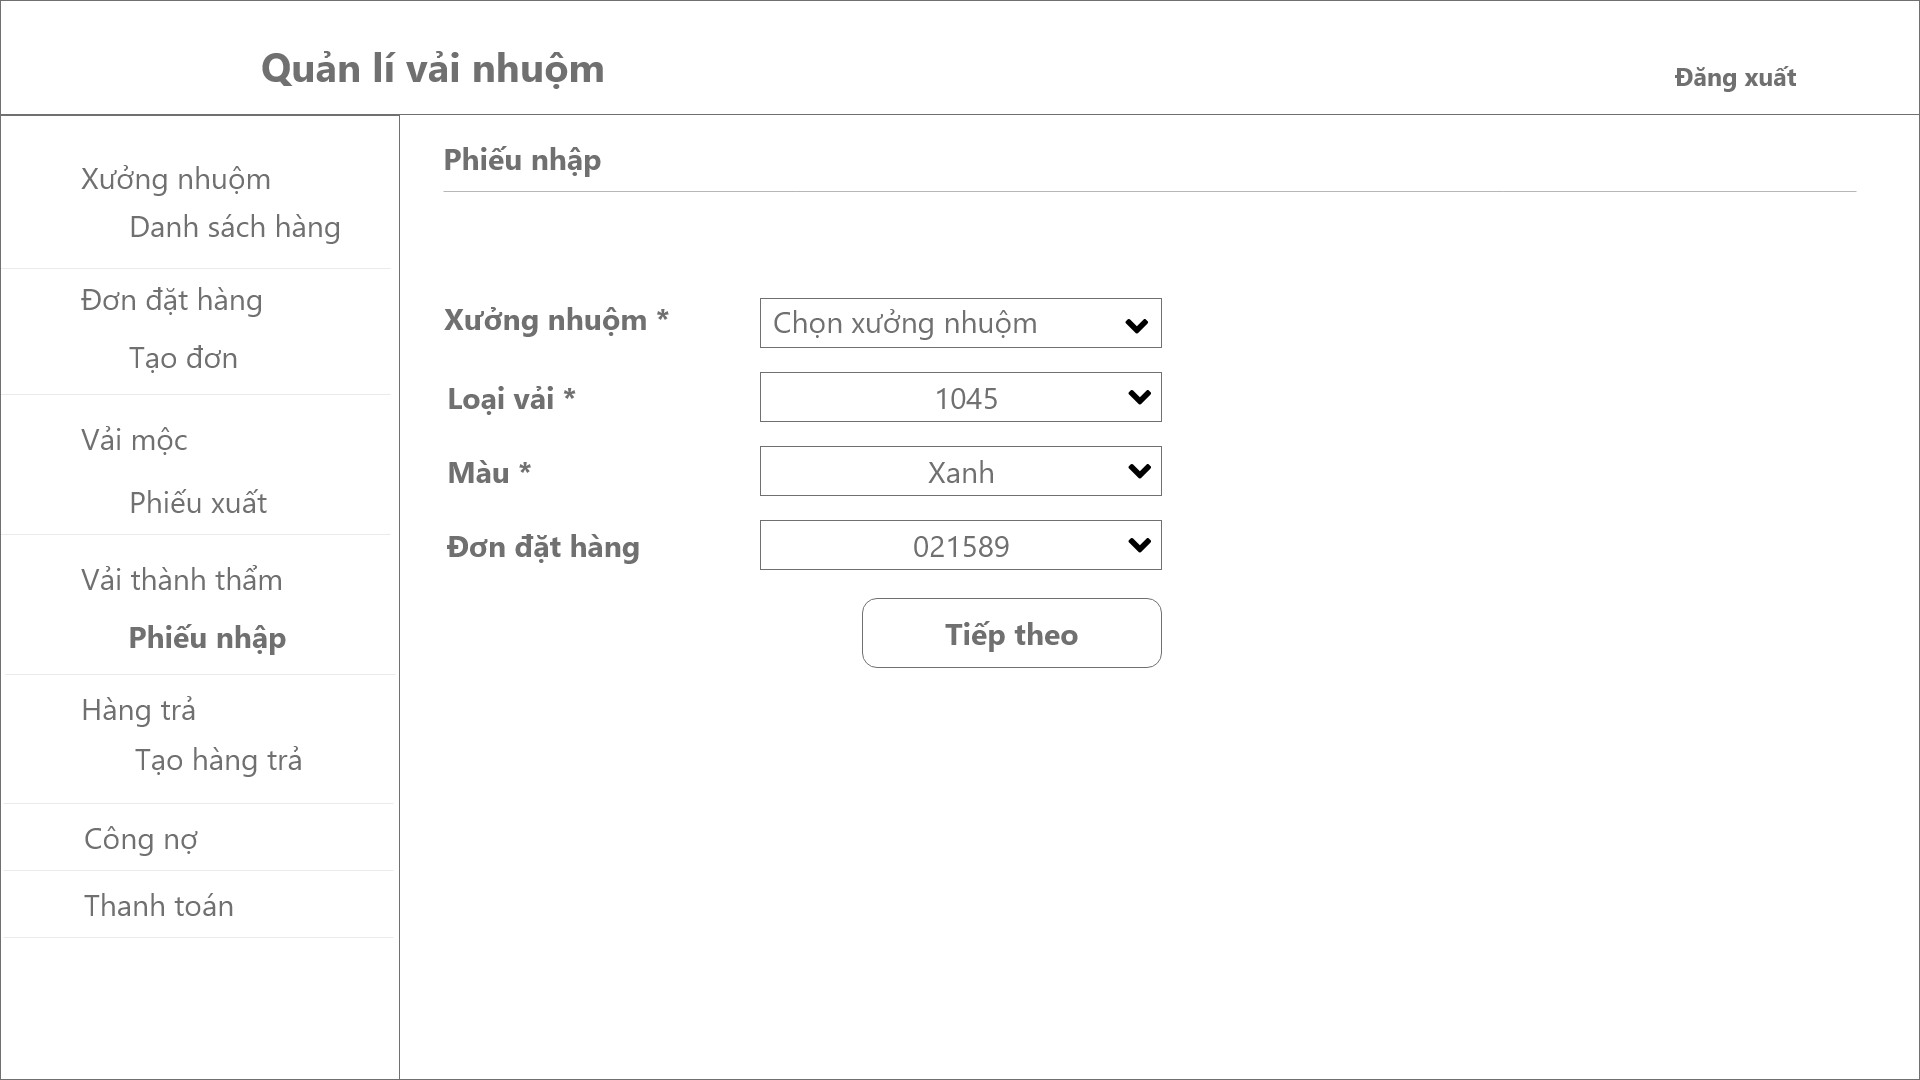
\includegraphics[width=12cm]{Image/Mockup/Tạo phiếu nhập - 1.png}}
        \caption{Tạo phiếu nhập thành phẩm - bước 1}
        \label{mockup_generate_import_1}
    \end{center}
\end{figure}

\begin{figure}[H]
    \begin{center}
        \frame{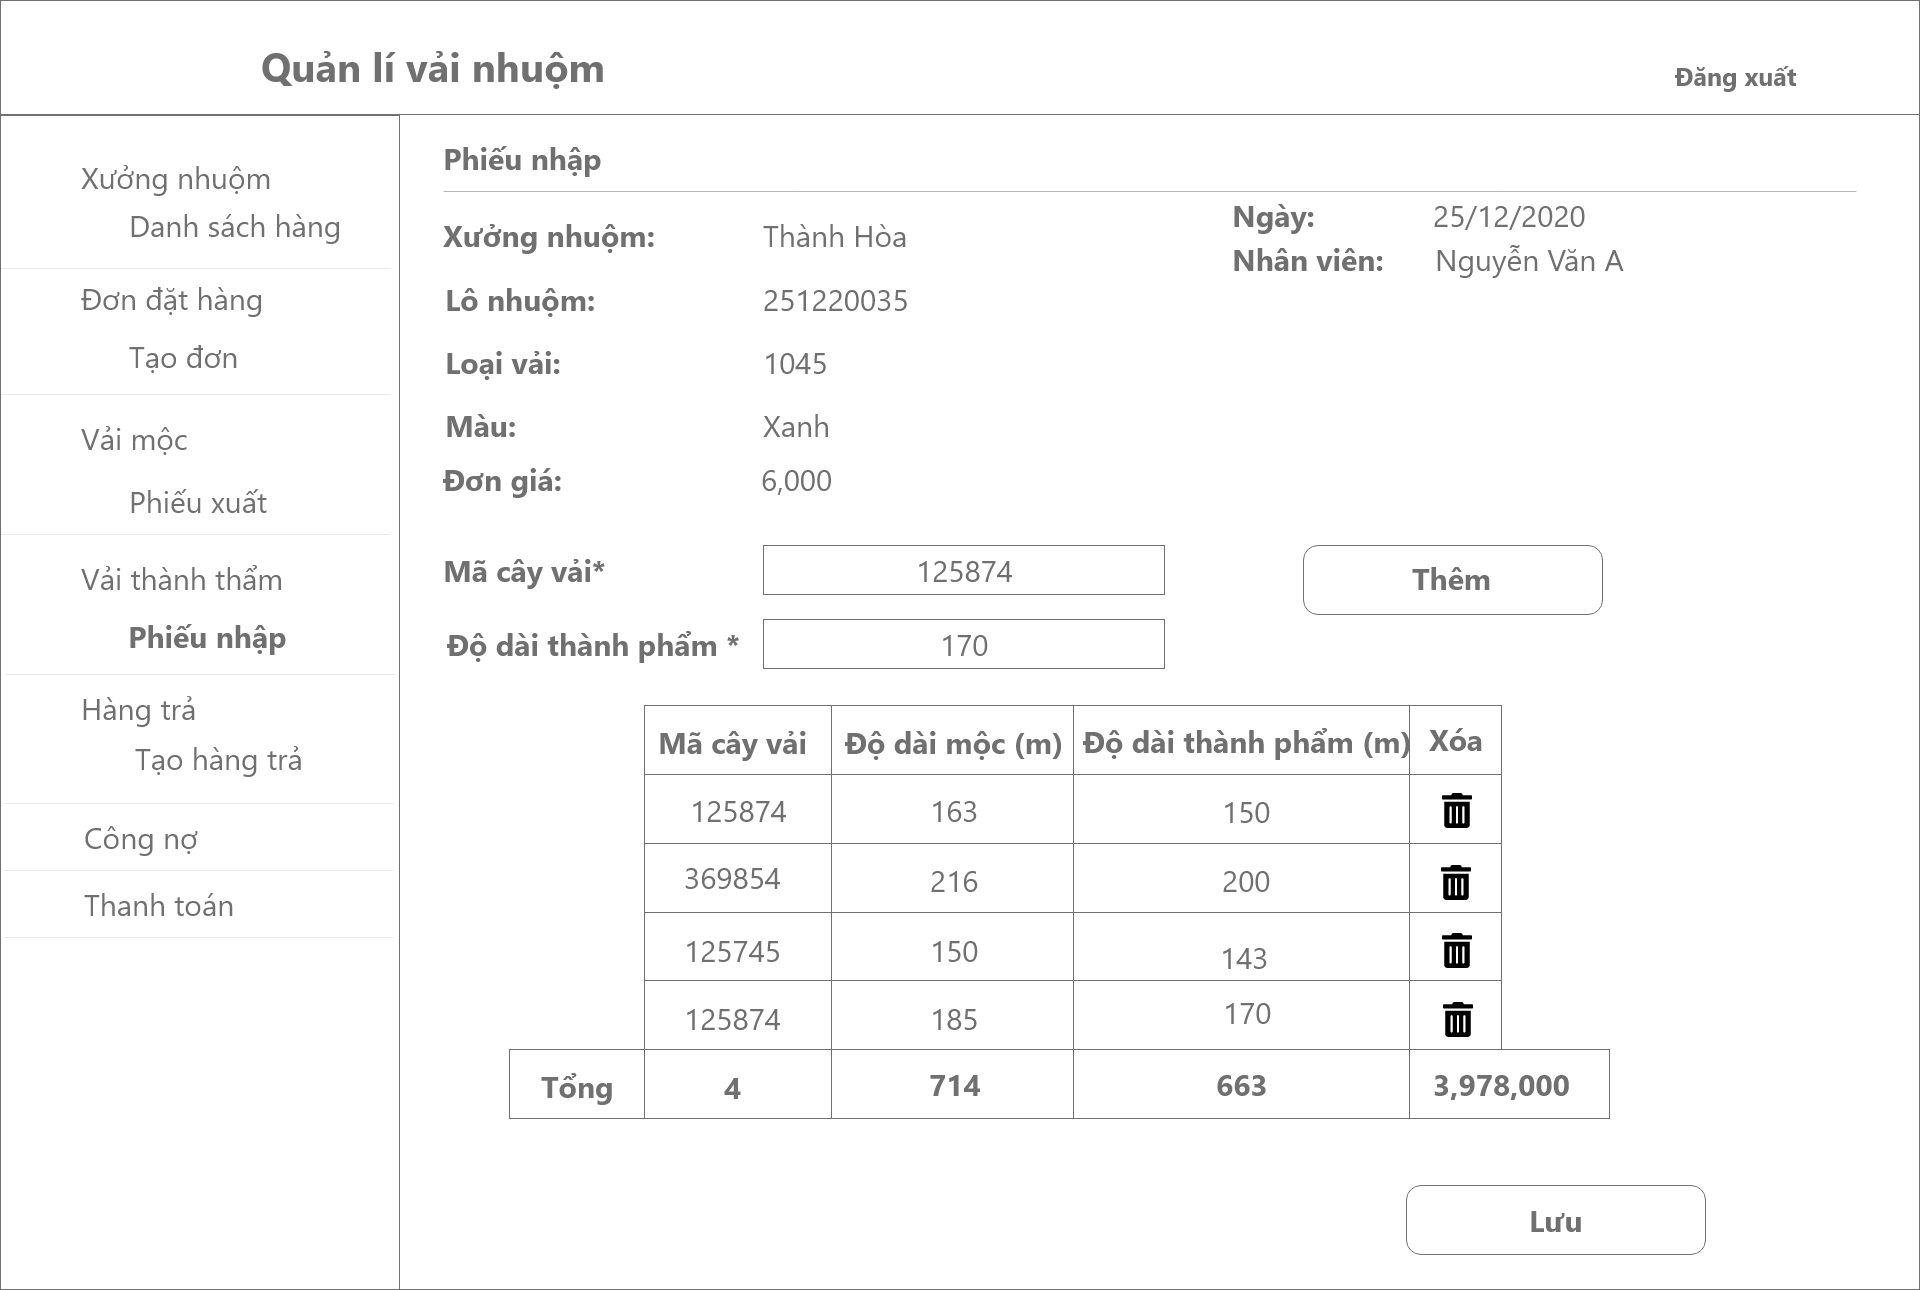
\includegraphics[width=12cm]{Image/Mockup/Tạo phiếu nhập - 2.png}}
        \caption{Tạo phiếu nhập thành phẩm - bước 2}
        \label{mockup_generate_import_2}
    \end{center}
\end{figure}

%%%%%%%%%%%%%%%%%%%%%%%%%%%%%%%%%%%%%%
\subsubsection{Quản lí hàng trả}

\begin{figure}[H]
    \begin{center}
        \frame{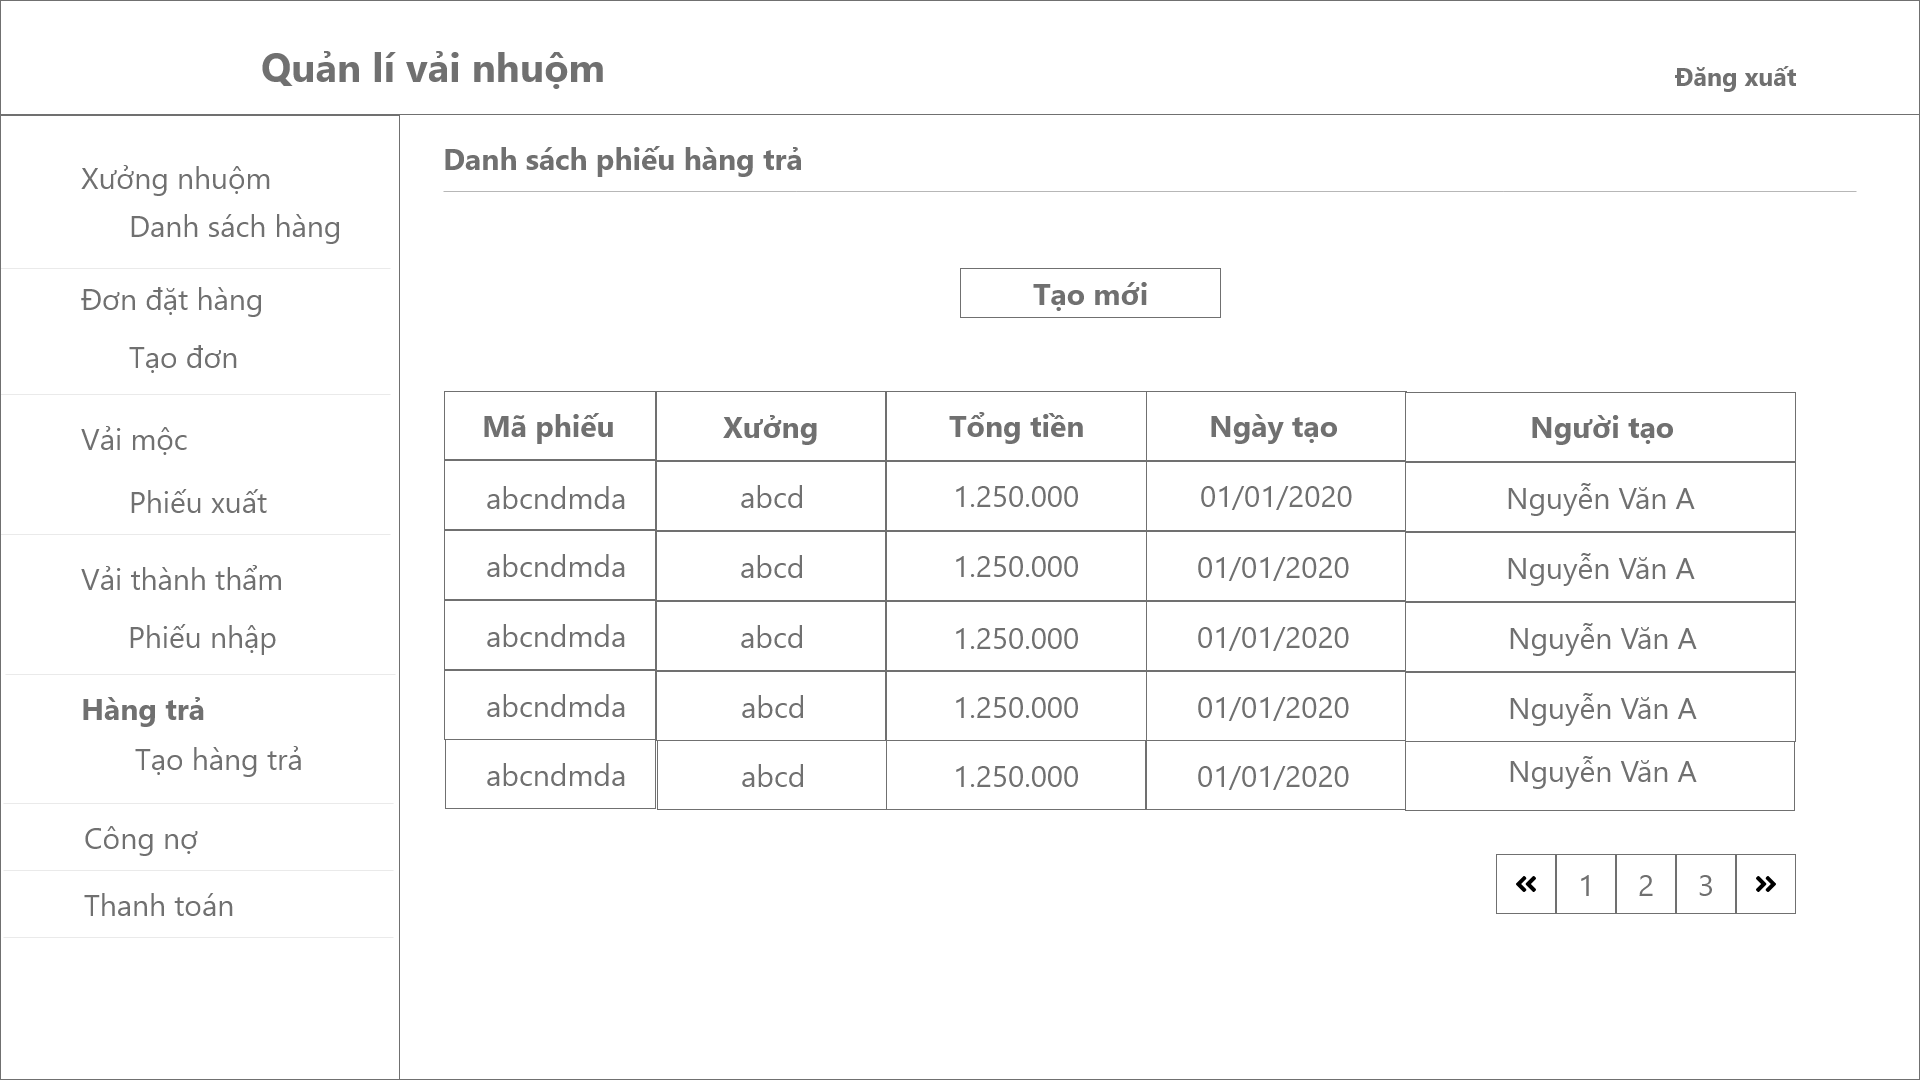
\includegraphics[width=12cm]{Image/Mockup/Danh sách hàng trả.png}}
        \caption{Danh sách phiếu hàng trả}
        \label{mockup_list_return_invoice}
    \end{center}
\end{figure}

\begin{figure}[H]
    \begin{center}
        \frame{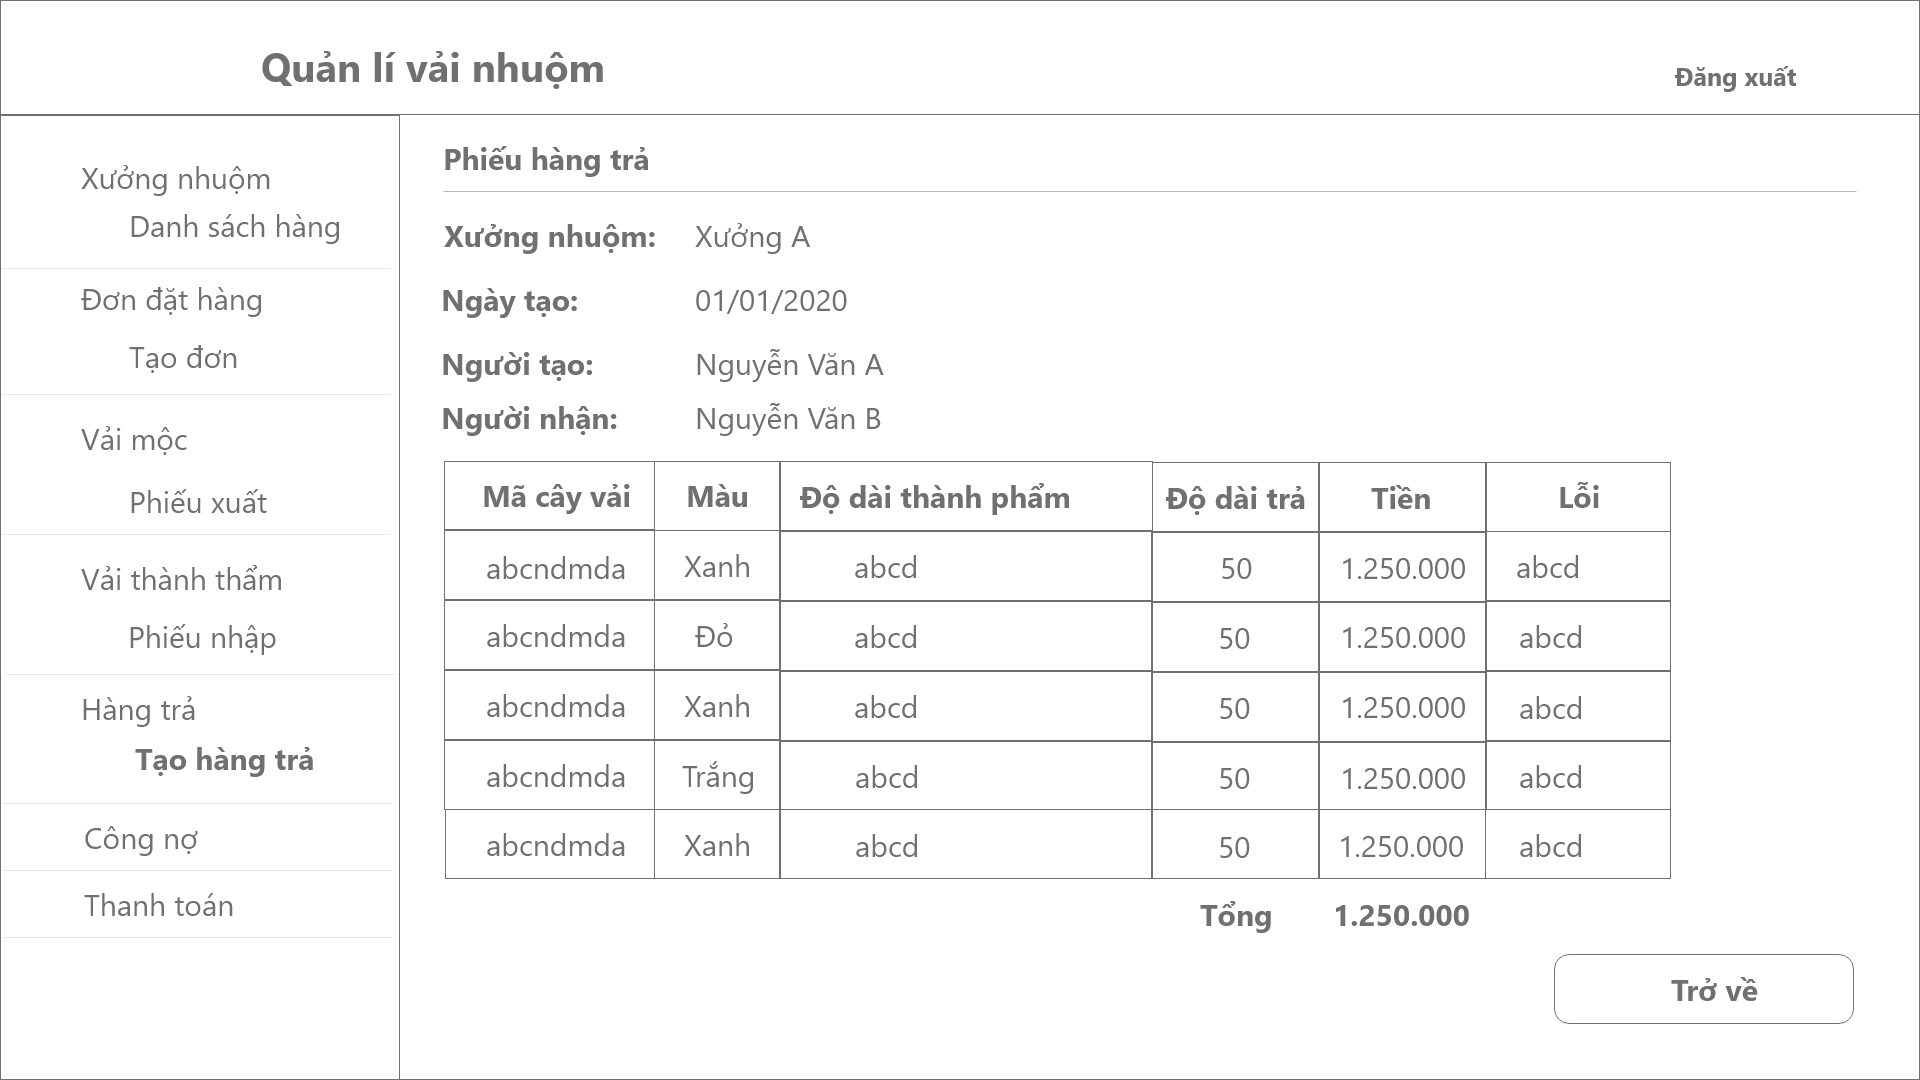
\includegraphics[width=12cm]{Image/Mockup/Chi tiết phiếu hàng trả.png}}
        \caption{Chi tiết phiếu hàng trả}
        \label{mockup_detail_return_invoice}
    \end{center}
\end{figure}

\begin{figure}[H]
    \begin{center}
        \frame{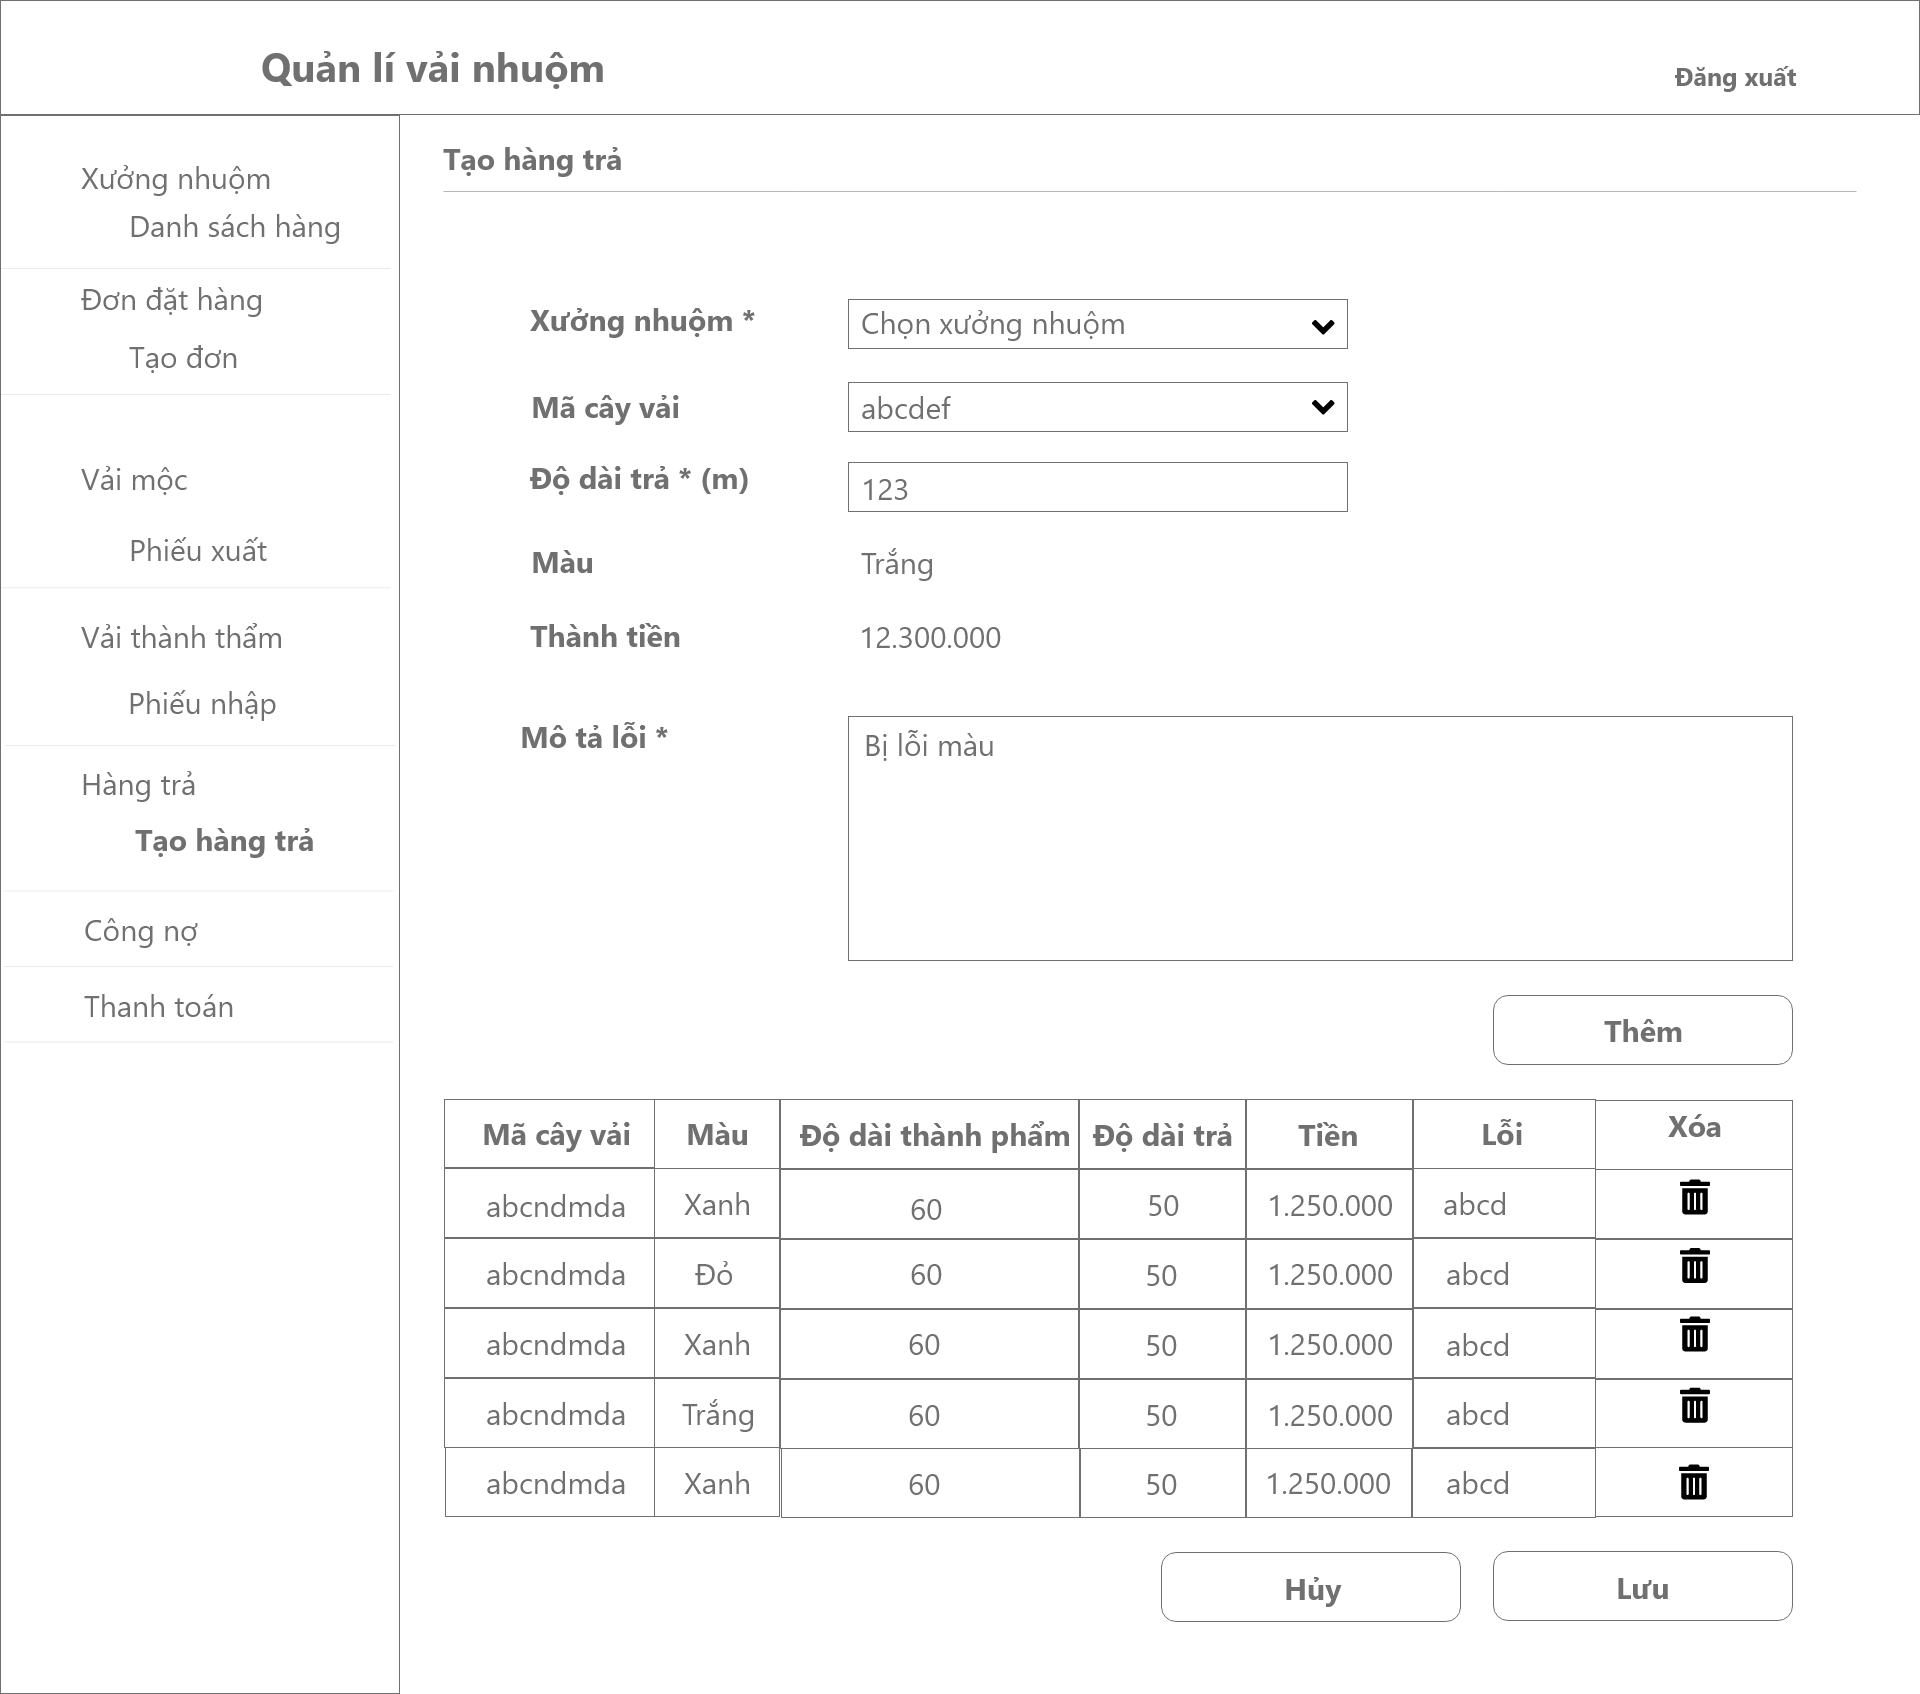
\includegraphics[width=12cm]{Image/Mockup/Tạo phiếu hàng trả.png}}
        \caption{Tạo phiếu hàng trả}
        \label{mockup_create_return_invoice_1}
    \end{center}
\end{figure}

%%%%%%%%%%%%%%%%%%%%%%%%%%%%%%%%%%%%%%%%%%%%%%
\subsubsection{Công nợ}

\begin{figure}[H]
    \begin{center}
        \frame{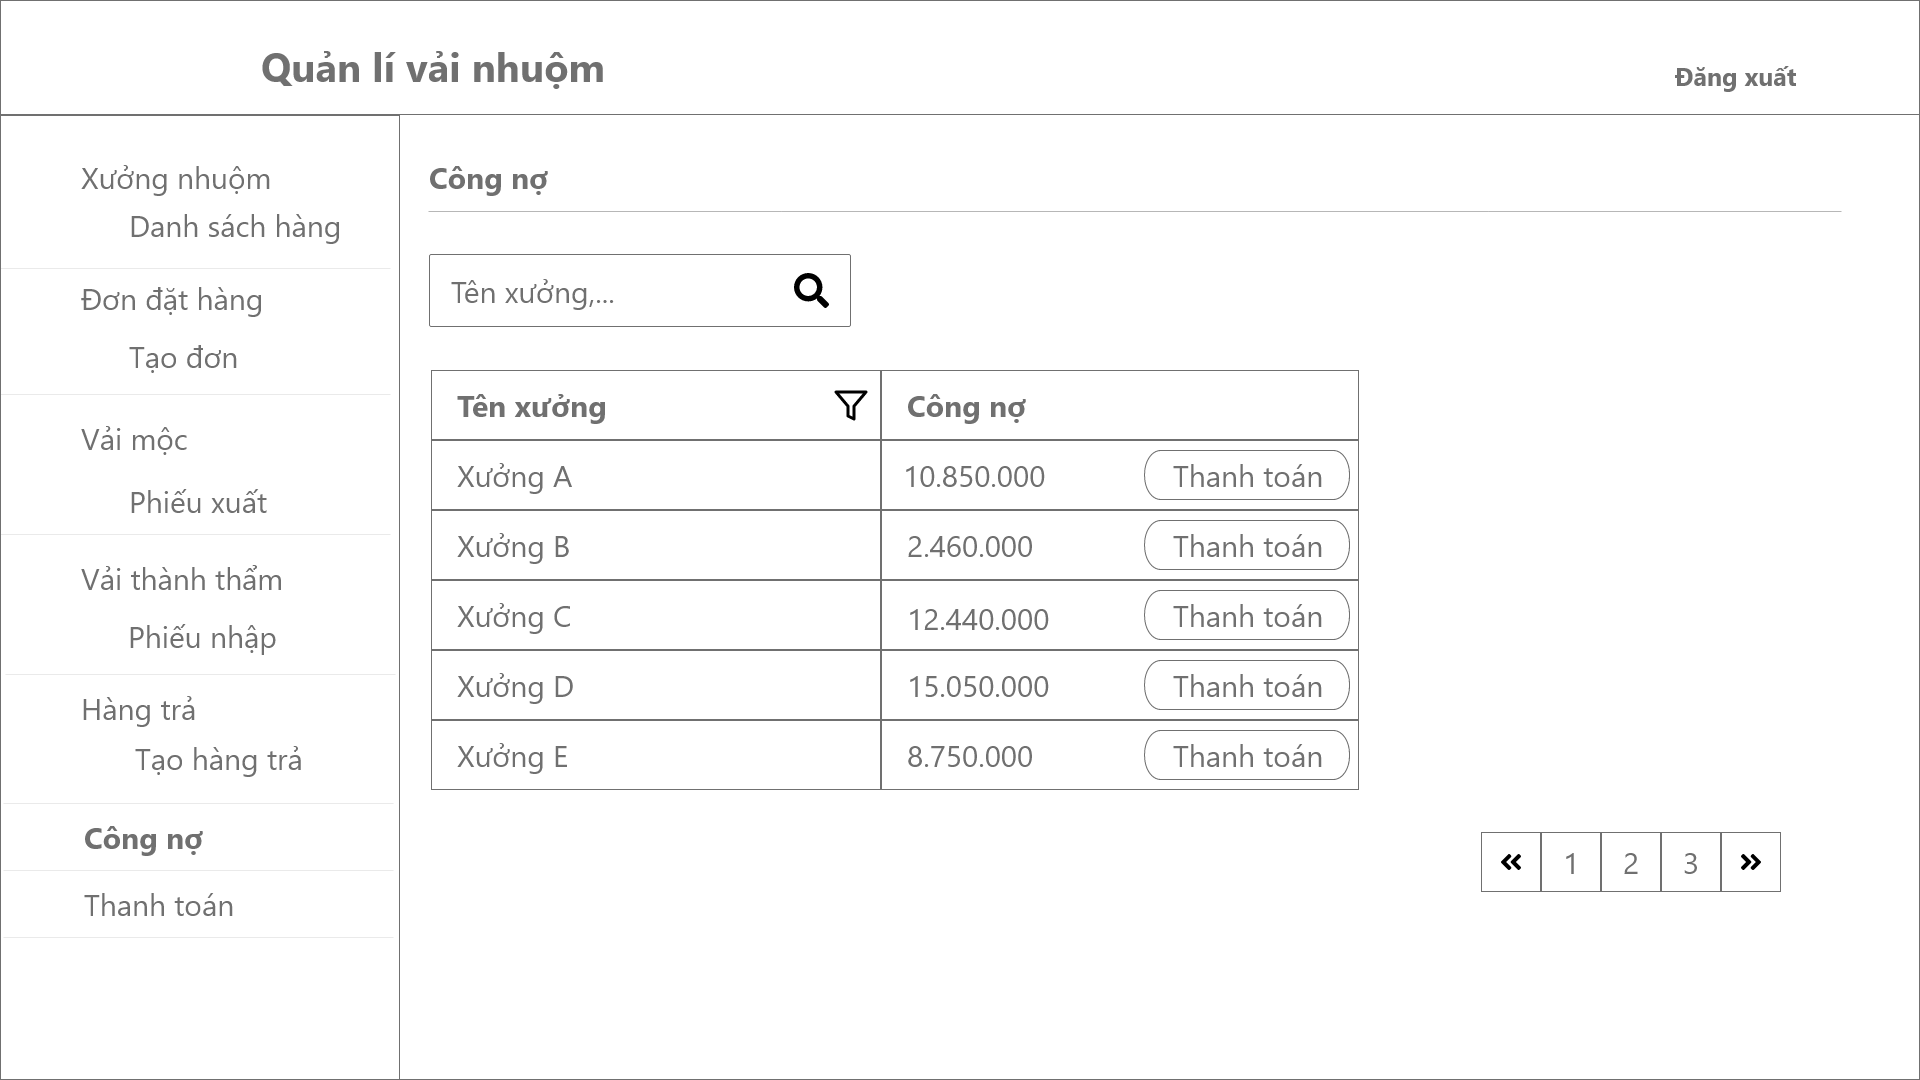
\includegraphics[width=12cm]{Image/Mockup/Công nợ.png}}
        \caption{Danh sách công nợ ở các xưởng}
        \label{mockup_debt}
    \end{center}
\end{figure}

%%%%%%%%%%%%%%%%%%%%%%%%%%%%%%%%%%%%%%%%%%%%%%
\subsubsection{Thanh toán}

\begin{figure}[H]
    \begin{center}
        \frame{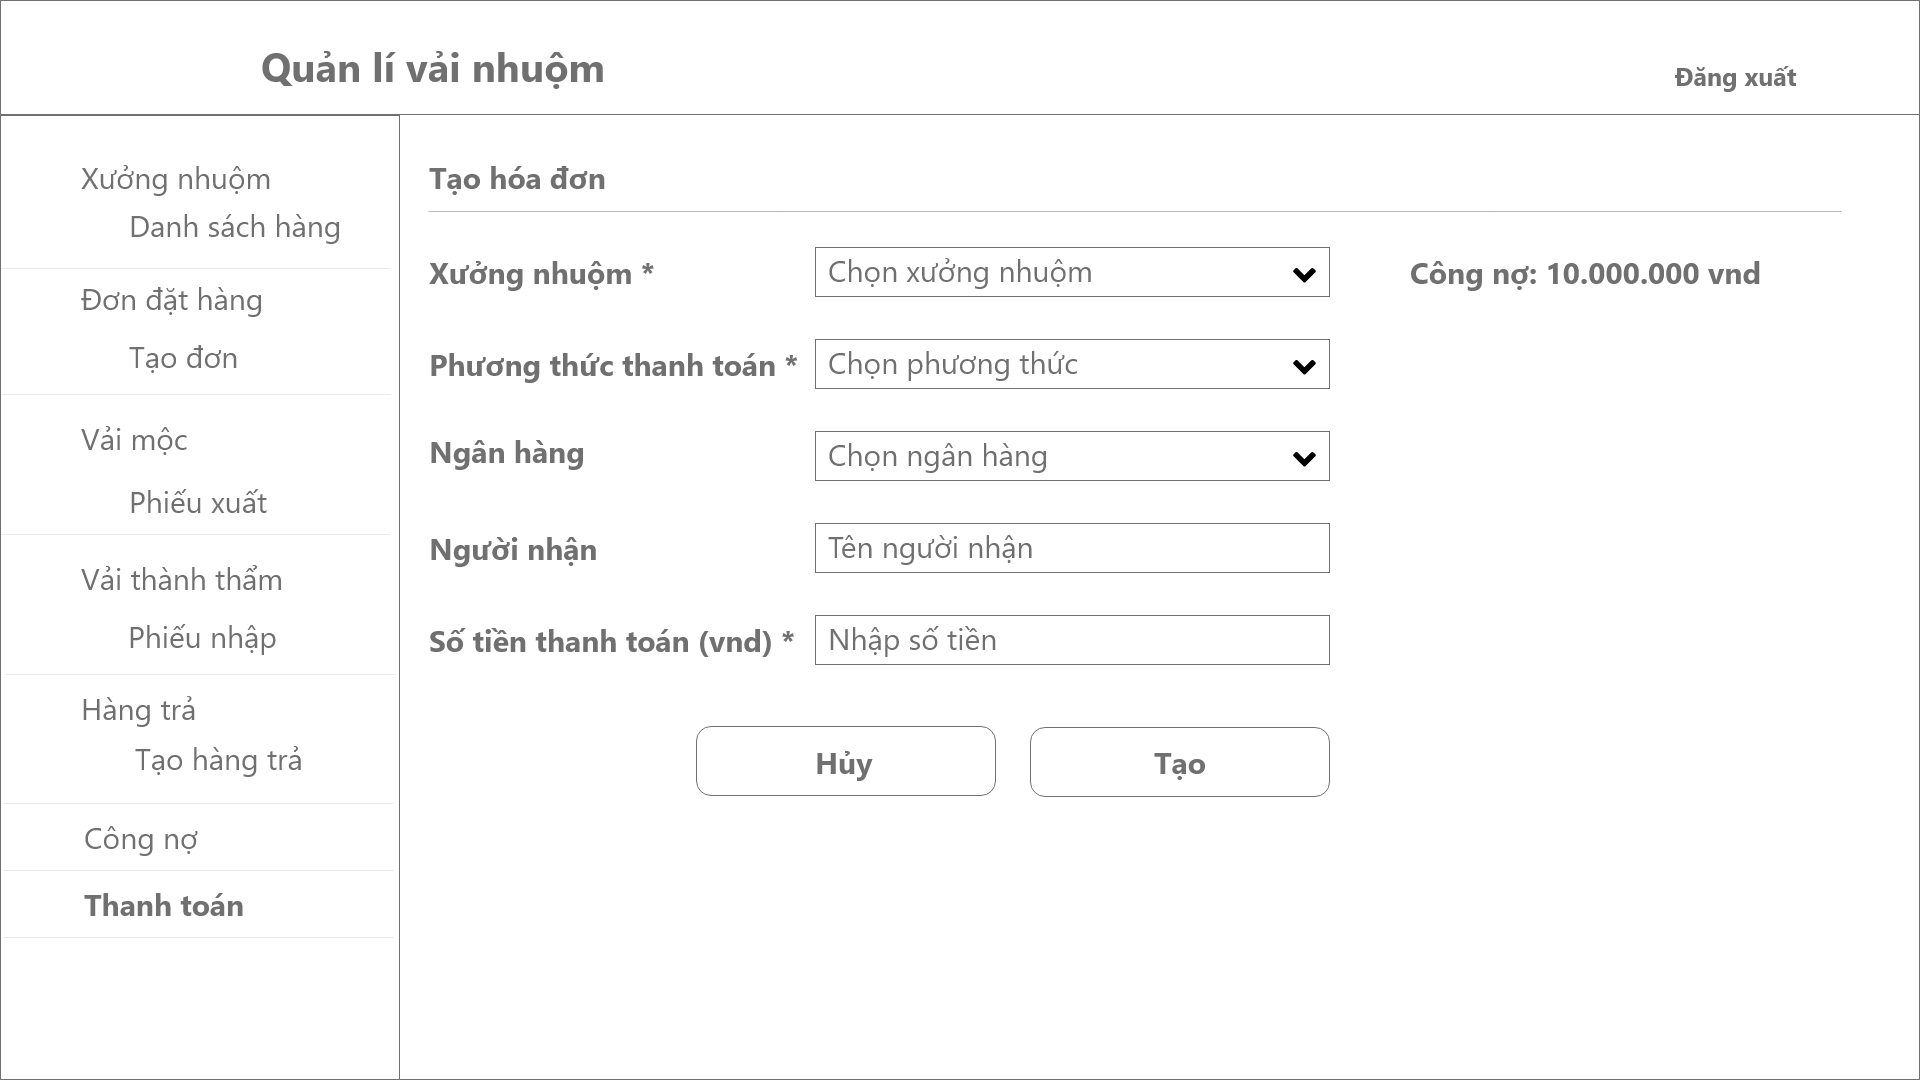
\includegraphics[width=12cm]{Image/Mockup/Tạo phiếu thanh toán.png}}
        \caption{Tạo hóa đơn thanh toán}
        \label{mockup_payment}
    \end{center}
\end{figure}

%%%%%%%%%%%%%%%%%%%%%%%%%%%%%%%%%
% \newpage
% \section{Kế hoạch luận văn}
% \input{Text/ke_hoach_luan_van}
%Lập bảng kế hoạch dựa trên GOM nhóm danh sách user story cho mỗi 2 tuần hiện thực

%%%%%%%%%%%%%%%%%%%%%%%%%%%%%%%%%
\newpage
\section{Hiện thực hệ thống}
\subsection{Công nghệ sử dụng}
Để xây dựng được một hệ thống lớn như vậy, nhóm đã sử dụng rất nhiều thư viện, framework như đã được giới thiệu trong Phần 2. Các công nghệ nổi bật được liệt kê dưới đây:

\begin{table}[h]
    \centering
    \begin{tabular}{|m{4cm}|m{2cm}|m{4cm}|}
    \hline 
        \textbf{Thư viện, framework} & \textbf{Phiên bản} & \textbf{Chức năng}\\ \hline
        React & 17.0.2 & Xây dựng giao diện \\ \hline
        Java & 1.8 & Môi trường runtime Java \\ \hline
        Spring & 2.4.3 & Xây dựng backend \\ \hline
        Maven & 3.6.3 & Quản lí thư viện \\ \hline
        Query DSL & 3.6.8 & Xây dựng các câu truy vấn \\ \hline
        JDBC & 2.4.3 & Kết nối database \\ \hline
        Lombok & 1.18.18 & Hỗ trợ sinh code tự động \\ \hline
        Postgre SQL & 13.3 & Hệ quản trị cơ sở dữ liệu \\ \hline
    \end{tabular}
    \caption{Công nghệ sử dụng.}
    \label{usedtech}
\end{table}

\subsection{Quản lí mã nguồn}
Để các thành viên trong nhóm có thể cùng nhau xây dựng hệ thống này một cách hiệu quả nhất, nhu cầu tất yếu phải có một hệ thống quản lý mã nguồn. Nhóm sử dụng \textbf{Git}, một hệ thống quản lý phiên bản phổ biến nhất hiện nay. \textbf{Git} giúp việc cộng tác dễ dàng hơn, cho phép thay đổi của các thành viên được hợp nhất thành một mã nguồn duy nhất.\par

Nhóm cũng sử dụng \textbf{Github}, một nền tảng lưu trữ mã nguồn của Git. Tất cả mã
nguồn của Luận văn tốt nghiệp được lưu trữ trên \textbf{Github}.


\subsection{Kết quả hiện thực}
Sau quá trình thực hiện luận văn, bằng cách sử dụng những công nghệ và kiên thức được đưa ra trong các phần trước, nhóm đã hoàn thành một Hệ thống quản lí vải nhuộm tương đối hoàn chỉnh.




%%%%%%%%%%%%%%%%%%%%%%%%%%%%%%%%%
\newpage
\section{Kế hoạch kiểm tra phần mềm}


%%%%%%%%%%%%%%%%%%%%%%%%%%%%%%%%%
\newpage
\section{Tổng kết}
\subsection{Kết quả đạt được}
% Qua quá trình thực hiện đề tài "Xây dựng một hệ thống quản lý quá trình gia công nhuộm cho một doanh nghiệp vải sợ trên nền web", nhóm đã đạt được rất nhiều kết quả đáng khích lệ. Từ những ngày đầu bắt tay vào làm đề tài, nhóm đã nghiên cứu, tìm hiểu về các chức năng, yêu cầu mà một hệ thống quản lý phải có. Một số kết quả mà nhóm đã đạt được:

\begin{itemize}
    \item Tìm hiểu thị trường và nhu cầu thực tế tương ứng với đề tài.
    \item Xây dựng được một hệ thống quản lý quá trình gia công nhuộm tương đối hoàn chỉnh ở cả hai phía client và server.
    \item Phân tích và thiết kế các chức năng từ việc phân tích yêu cầu, thiết kế usecase, thiết kế cơ sở dữ liệu: ERD, Relation Data Model.
    \item Giao diện đẹp, thân thiện và dễ dàng sử dụng.
    \item Có đầy đủ tính năng mà một hệ thống  quản lý phải có. Là một nền tảng giúp doanh nghiệp sản xuất vải sợi có thể quản lí quá trình gia công nhuộm.
    \item Sử dụng được những công nghệ đang rất nổi bật hiện nay như: ReactJS, Spring, Hibernate,... vào hệ thống.
    \item Thiết kế hệ thống theo dạng module, dễ dàng tích hợp và mở rộng sau này
\end{itemize}

\subsection{Hạn chế}
% Bên cạnh những kết quả đã đạt được, vì điều kiện thời gian và thành viên còn hạn chế, đề tài nhóm thực hiện vẫn cần phải cải thiện rất nhiều. Một số nhược điểm như:
\begin{itemize}
    \item Mã nguồn hệ thống vẫn chưa được tối ưu nhất.
    \item Chưa tìm hiểu về tích hợp các công cụ hay thư viện bên ngoài để hỗ trợ việc quản lí.
    \item Chưa có cơ hội tích hợp với các hệ thống khác.
\end{itemize}

	
%%%%%%%%%%%%%%%%%%%%%%%%%%%%%%%%%
\newpage
\addcontentsline{toc}{section}{Tài liệu tham khảo}
\begin{thebibliography}{80}

\bibitem{Databse} Ramez Elmasri, Shamkant B. Navathe (2016), \textit{Fundamentals of Database Systems}, \textit{7th Edition}, Pearson.

\bibitem{Postgre SQL, } Postgre SQL, https://www.postgresql.org/docs/13/index.html

\bibitem{software} Ian Sommerville (2016), \textit{Software Engineering}, \textit{10th Edition}, Pearson.

\bibitem{Java core} Java core, https://www.tutorialspoint.com/java/index.htm

\bibitem{Java spring boot} Java spring boot, https://spring.io/projects/spring-boot

\bibitem{Spring JDBC} Spring JDBC, https://www.baeldung.com/spring-jdbc-jdbctemplate

\bibitem{Spring Lombok} Spring Lombok, https://www.baeldung.com/lombok-accessors

\bibitem{Query DSL} Query DSL https://www.elastic.co/guide/en/elasticsearch/reference/current/query-dsl.html

\bibitem{Send email} Send email, https://www.tutorialspoint.com/spring\_boot/spring\_boot\_sending\_email.htm

\bibitem{Connect Postgre SQL} Connect Postgre SQL, https://www.baeldung.com/spring-boot-postgresql-docker

\bibitem{Generate SHA-256 hash} Generate SHA-256 hash, https://www.baeldung.com/sha-256-hashing-java

\bibitem{Generate token base64} Generate token base64, https://www.baeldung.com/java-base64-encode-and-decode

\bibitem{} Material-UI: Apopular React UI framework, https://material-ui.com/. 

\bibitem{} Exemplary real world application built with React + Redux, https://github.com/gothinkster/react-redux-realworld-example-app. 

\end{thebibliography}
\end{document}

